\begin{figure}[H]
\begin{center}
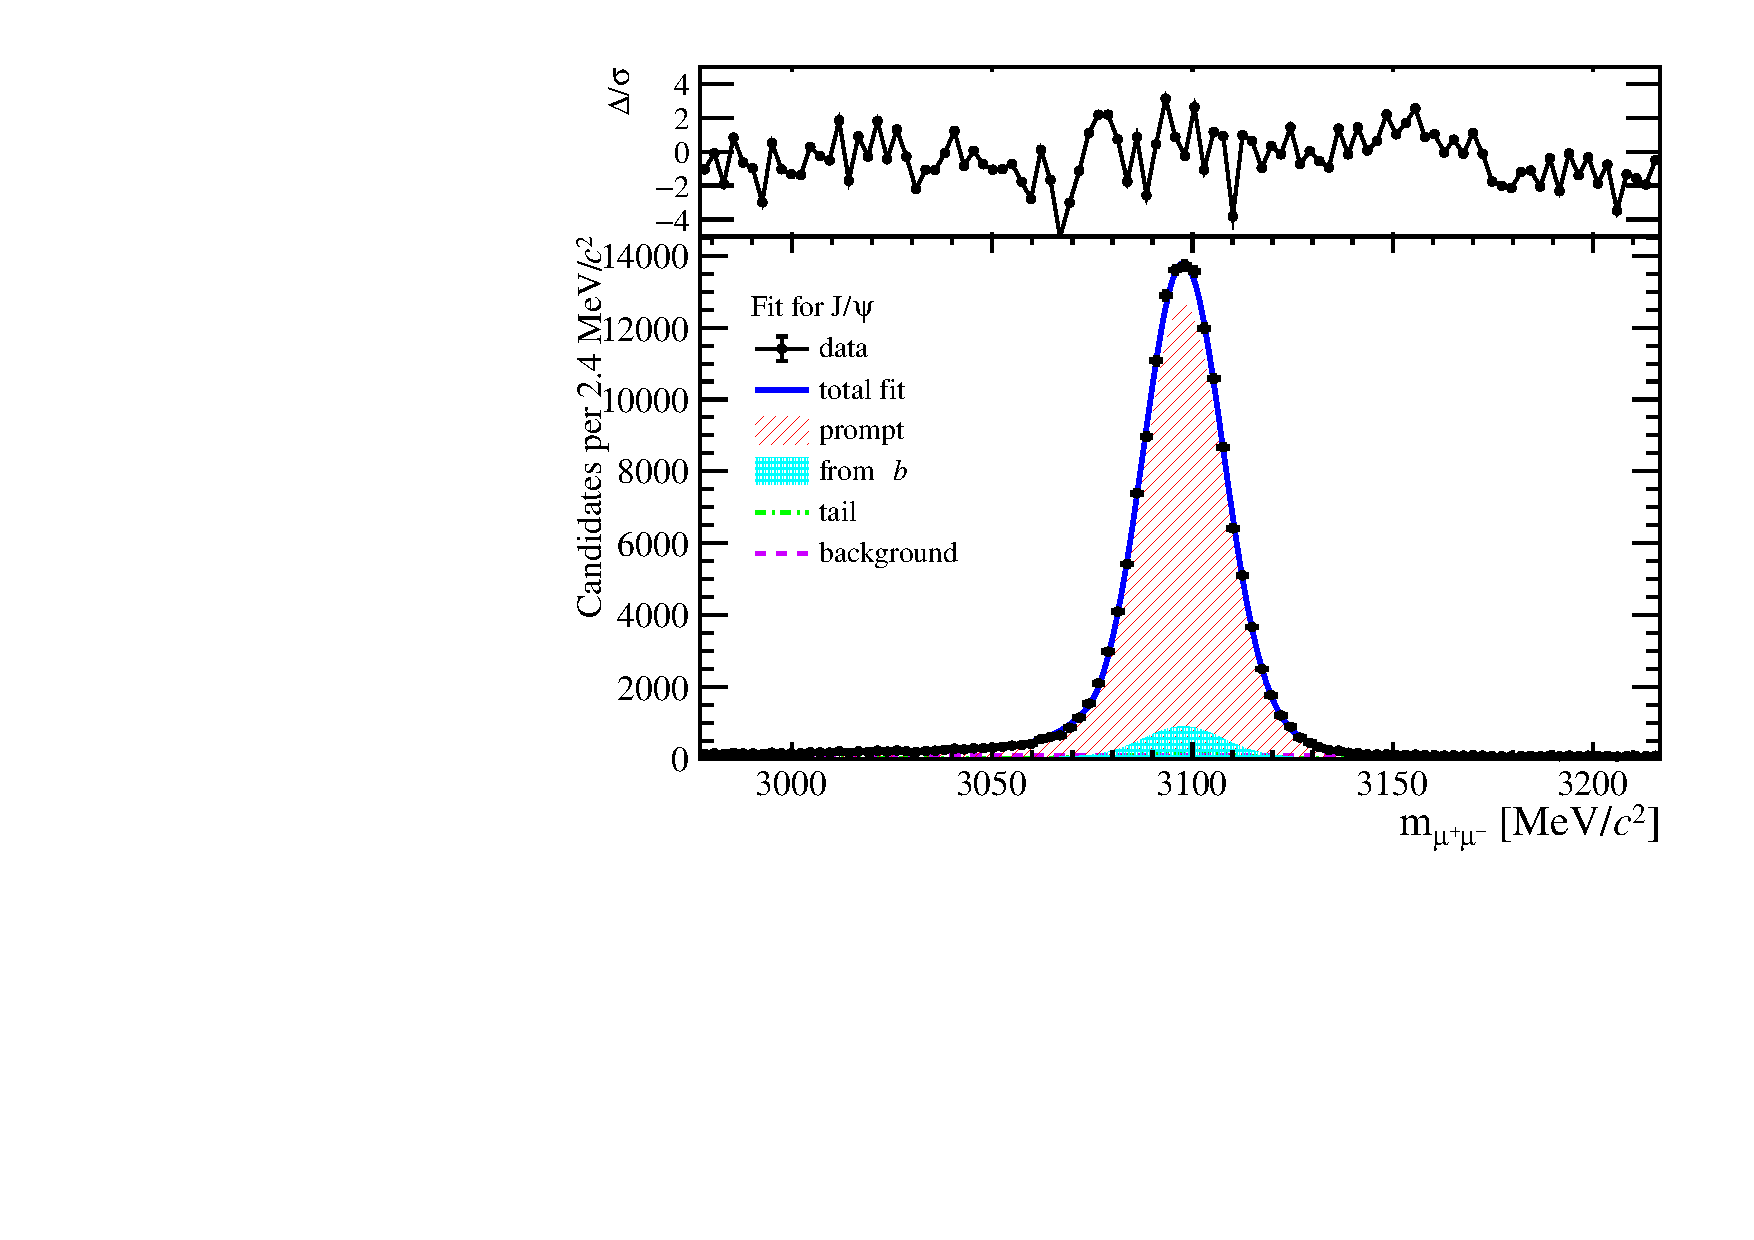
\includegraphics[width=0.47\linewidth]{pdf/Jpsi/drawmassF/n1y1pt1.pdf}
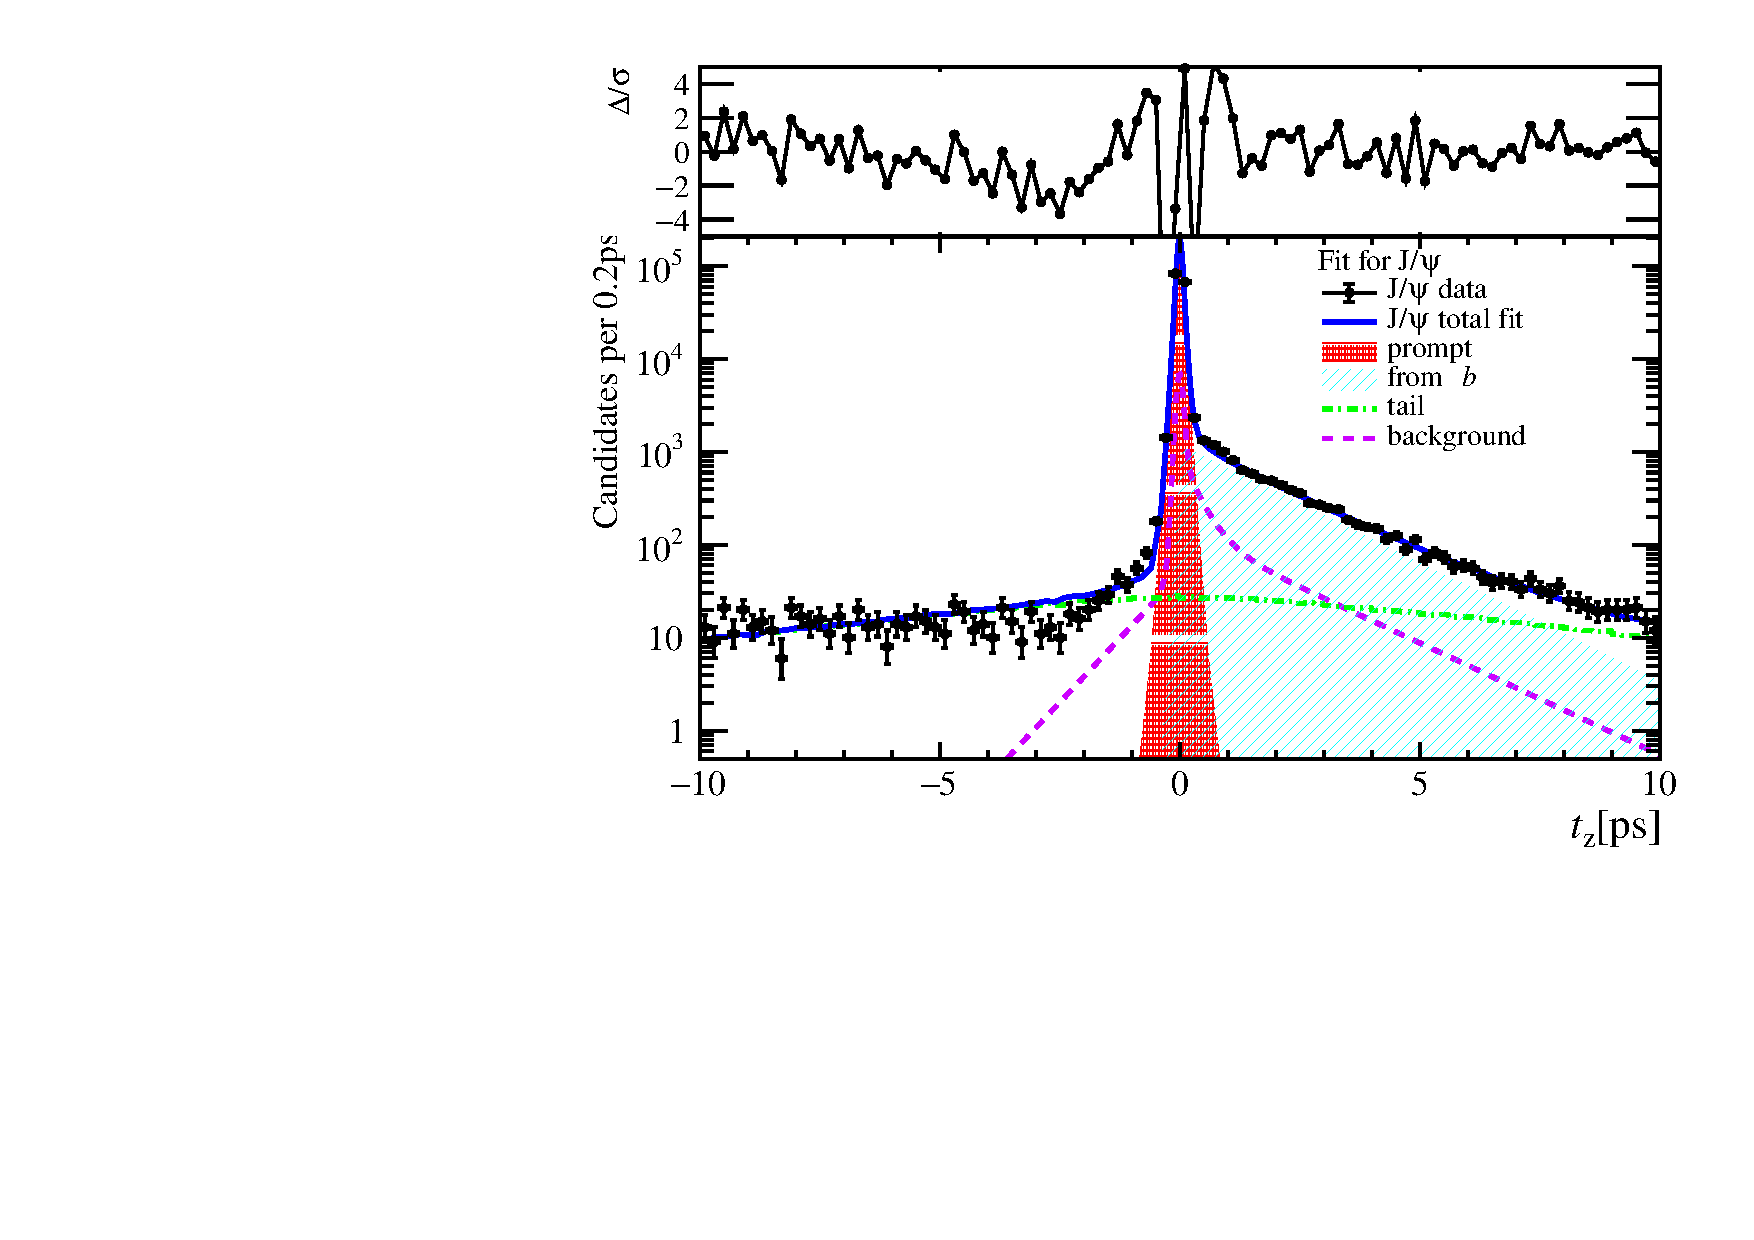
\includegraphics[width=0.47\linewidth]{pdf/Jpsi/2DFitF/n1y1pt1.pdf}
\vspace*{-0.5cm}
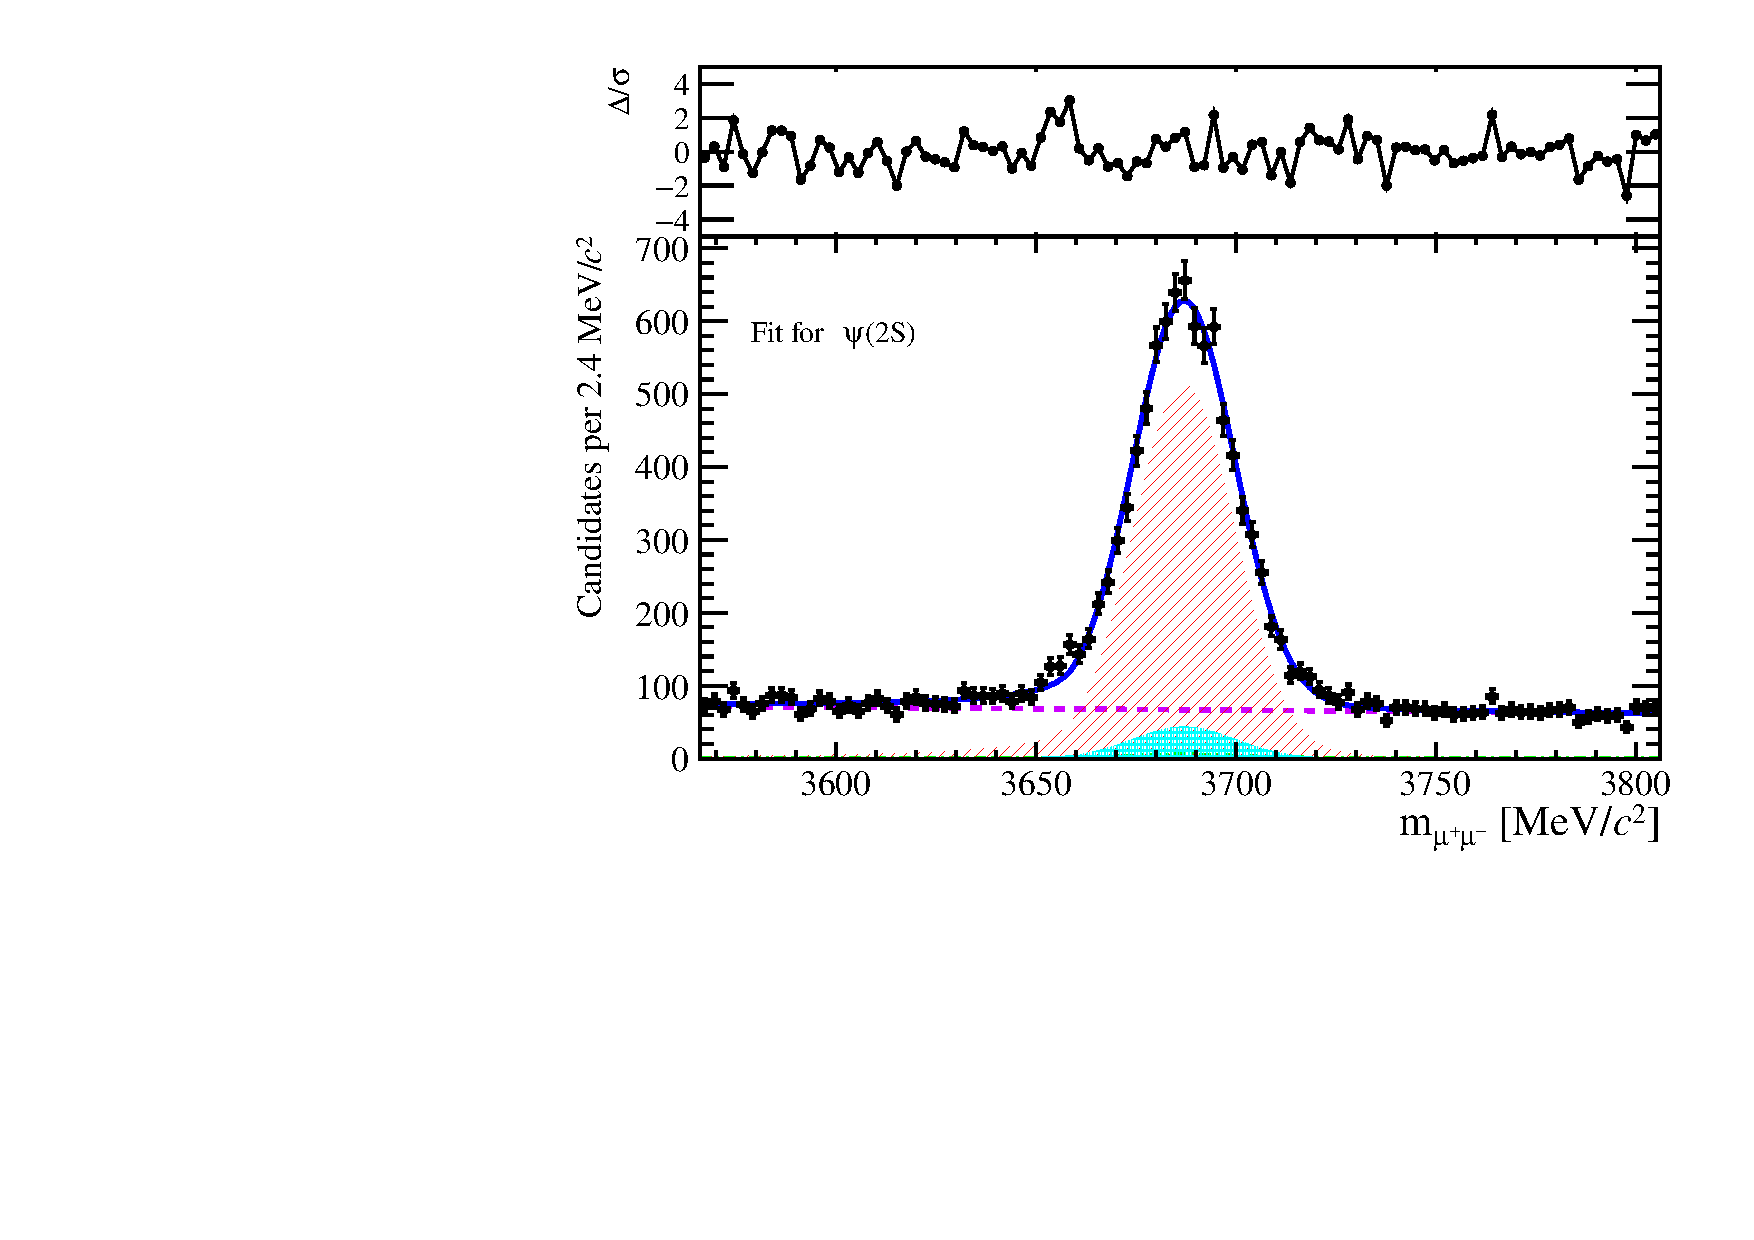
\includegraphics[width=0.47\linewidth]{pdf/Psi2S/drawmassF/n1y1pt1.pdf}
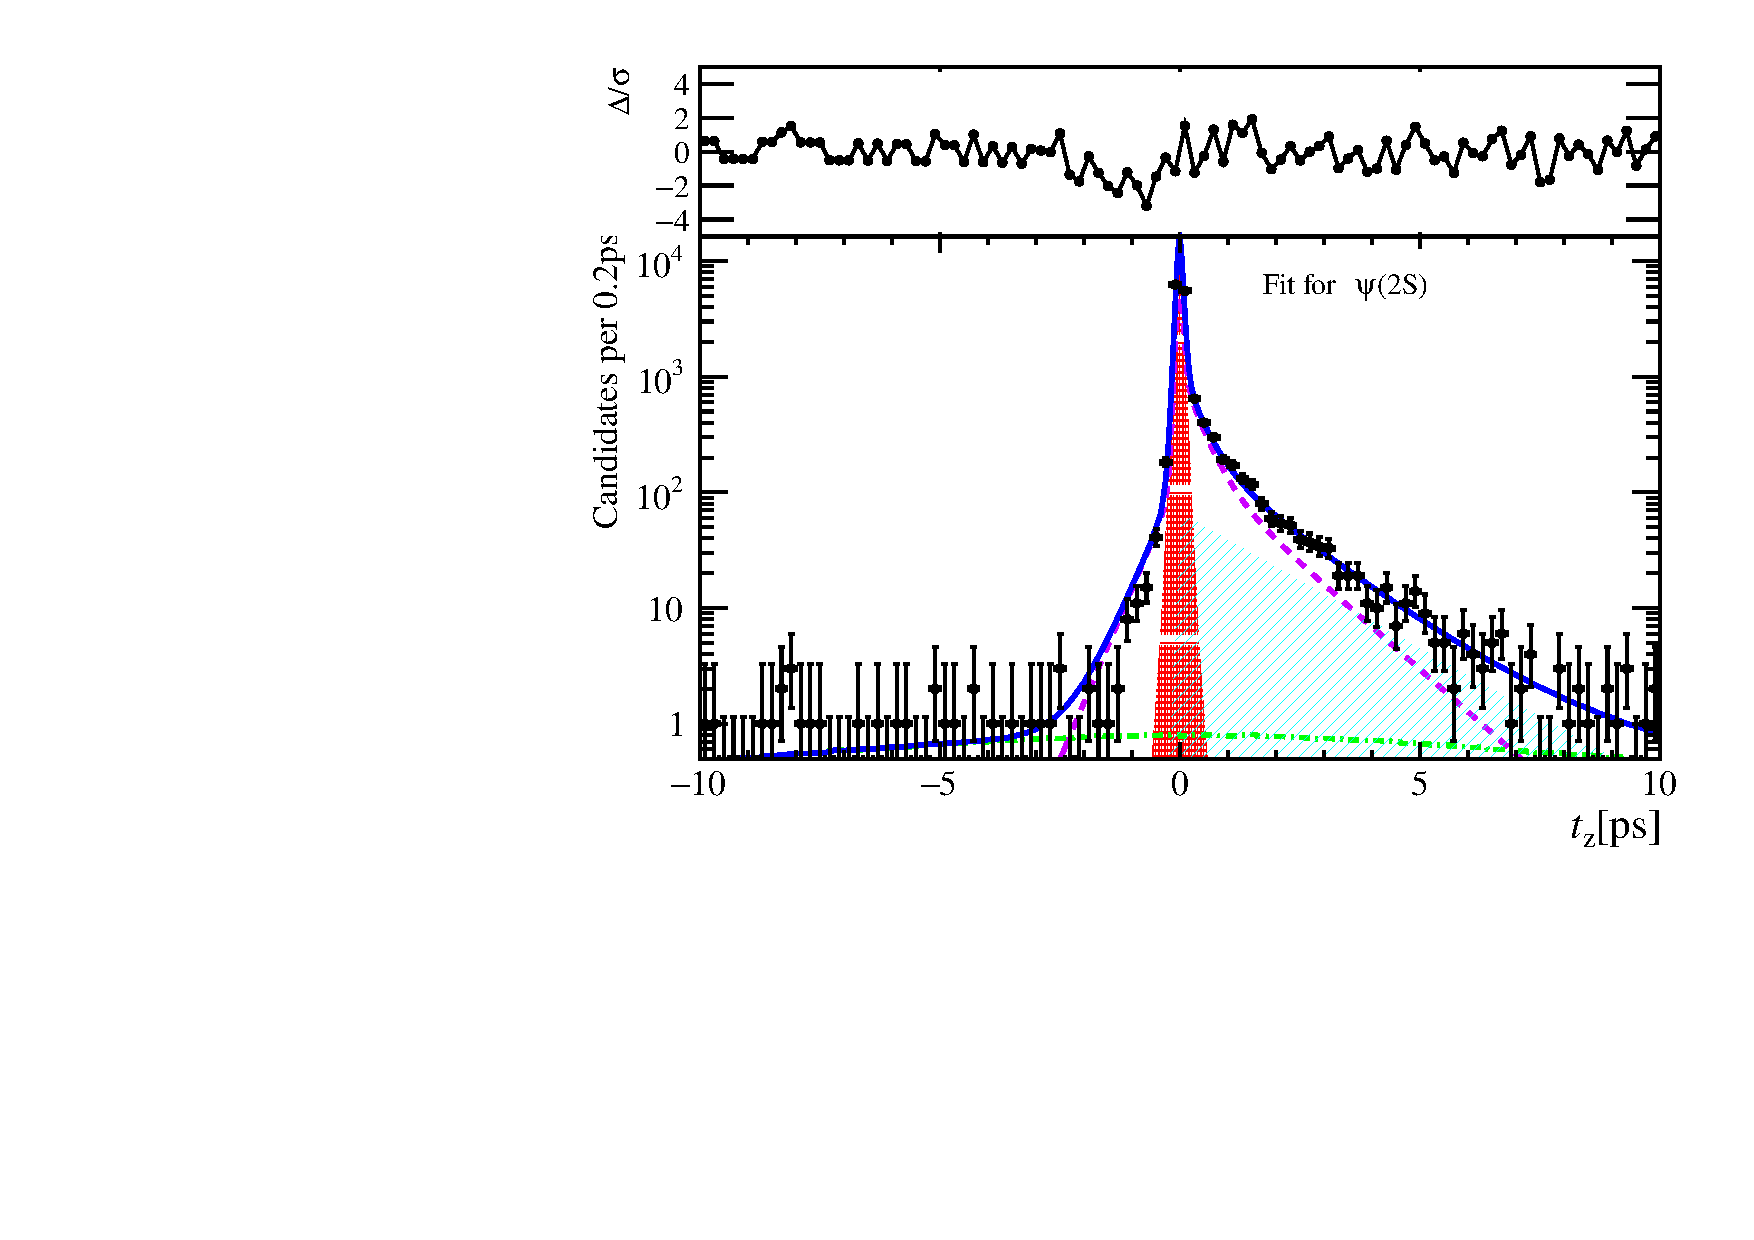
\includegraphics[width=0.47\linewidth]{pdf/Psi2S/2DFitF/n1y1pt1.pdf}
\vspace*{-0.5cm}
\end{center}
\caption{Fit results in $0\gevc<\pt<2\gevc$, $2.0<y<2.8$ and 0$\leq$nForwardTracks$<$12.}
\label{Fitn1y1pt1}
\end{figure}
\begin{figure}[H]
\begin{center}
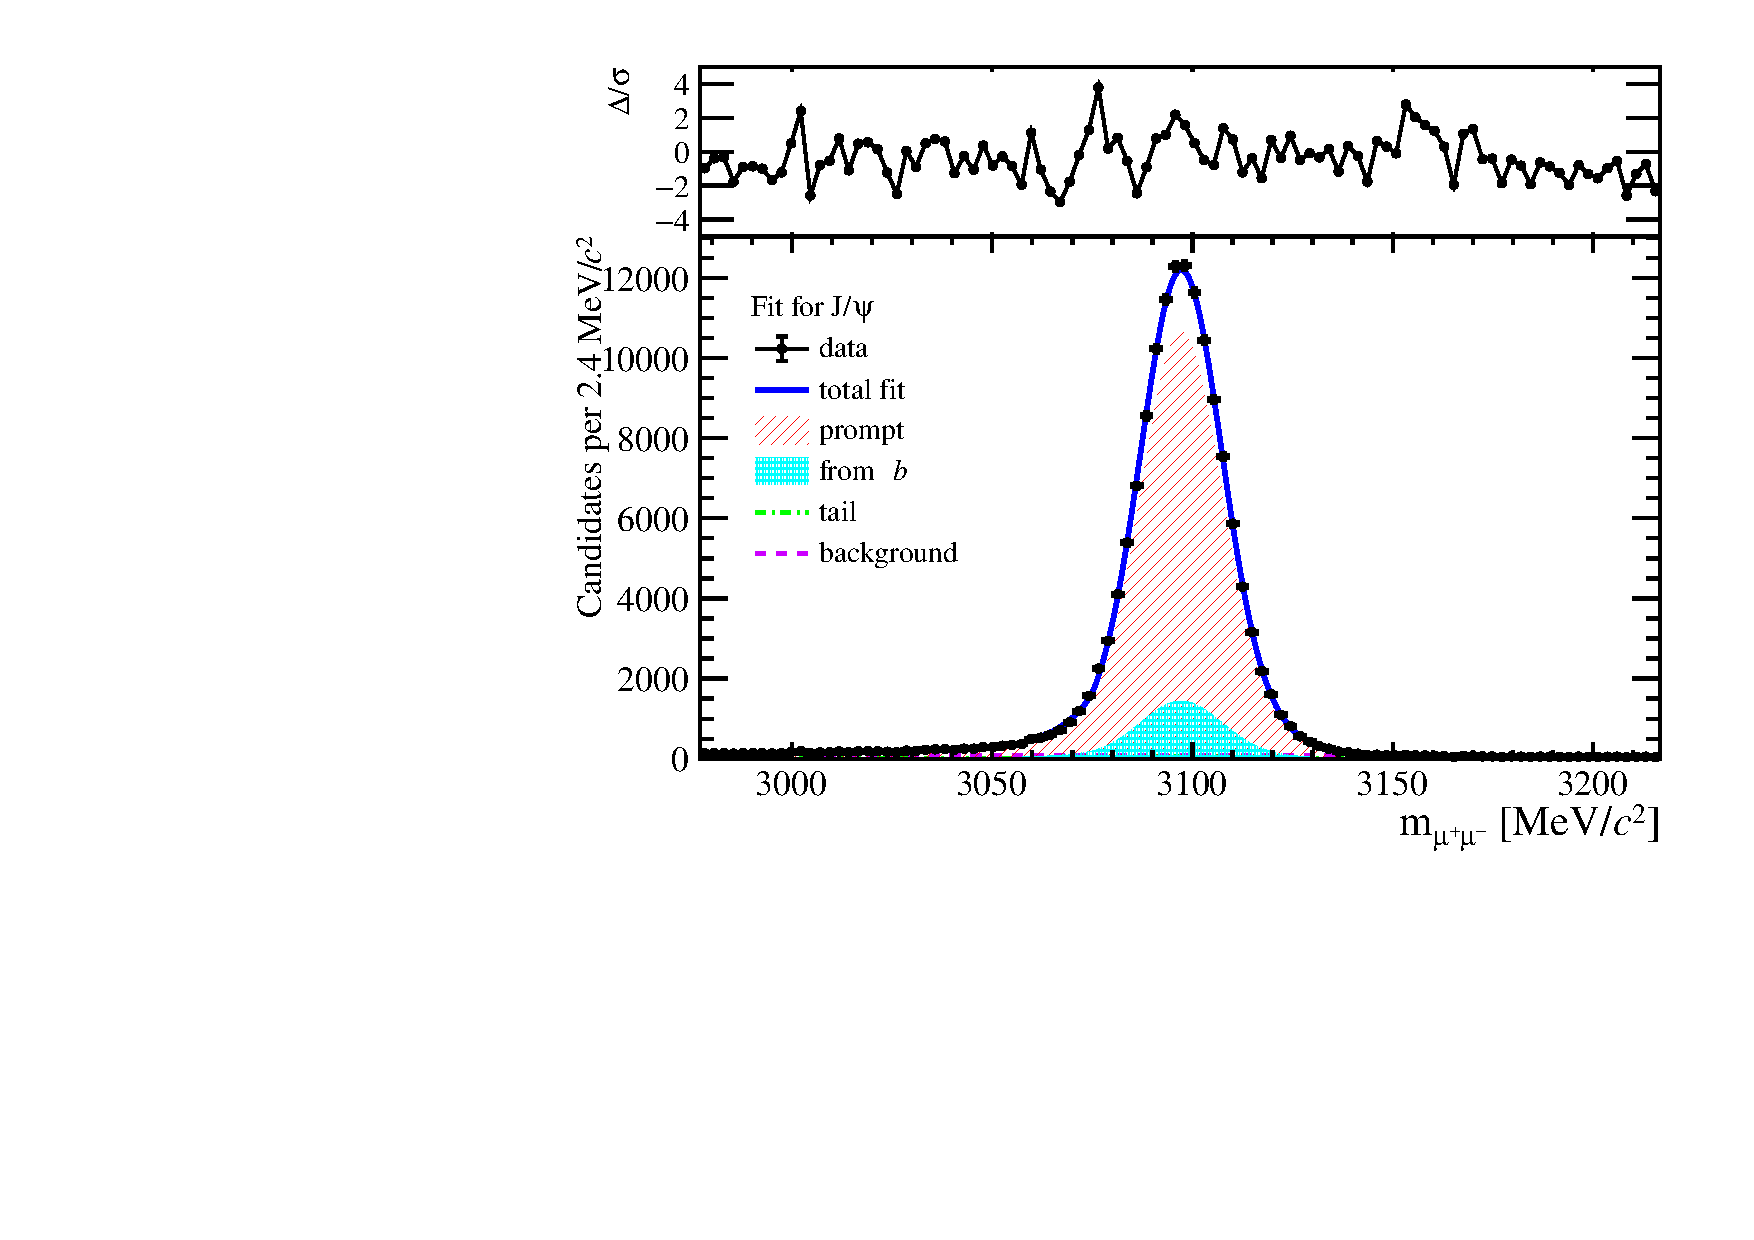
\includegraphics[width=0.47\linewidth]{pdf/Jpsi/drawmassF/n1y1pt2.pdf}
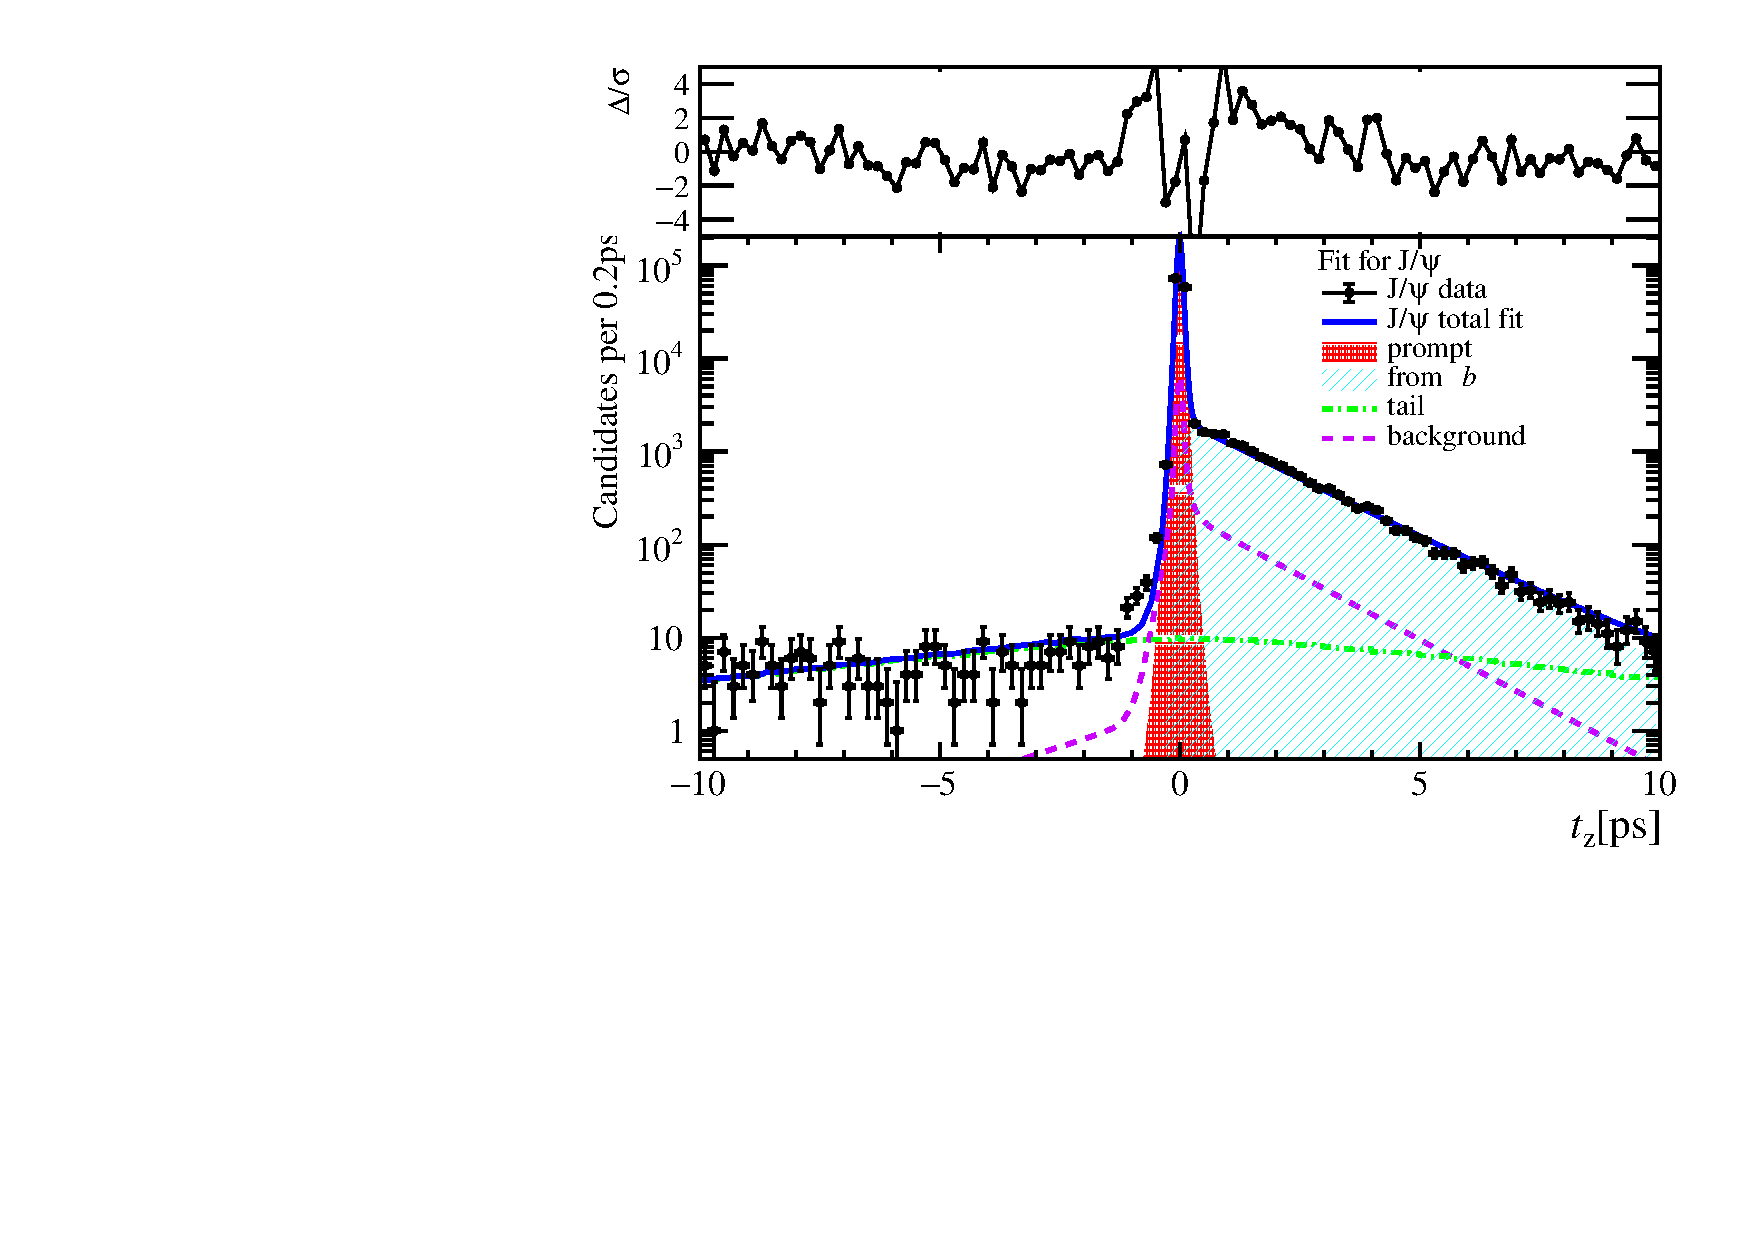
\includegraphics[width=0.47\linewidth]{pdf/Jpsi/2DFitF/n1y1pt2.pdf}
\vspace*{-0.5cm}
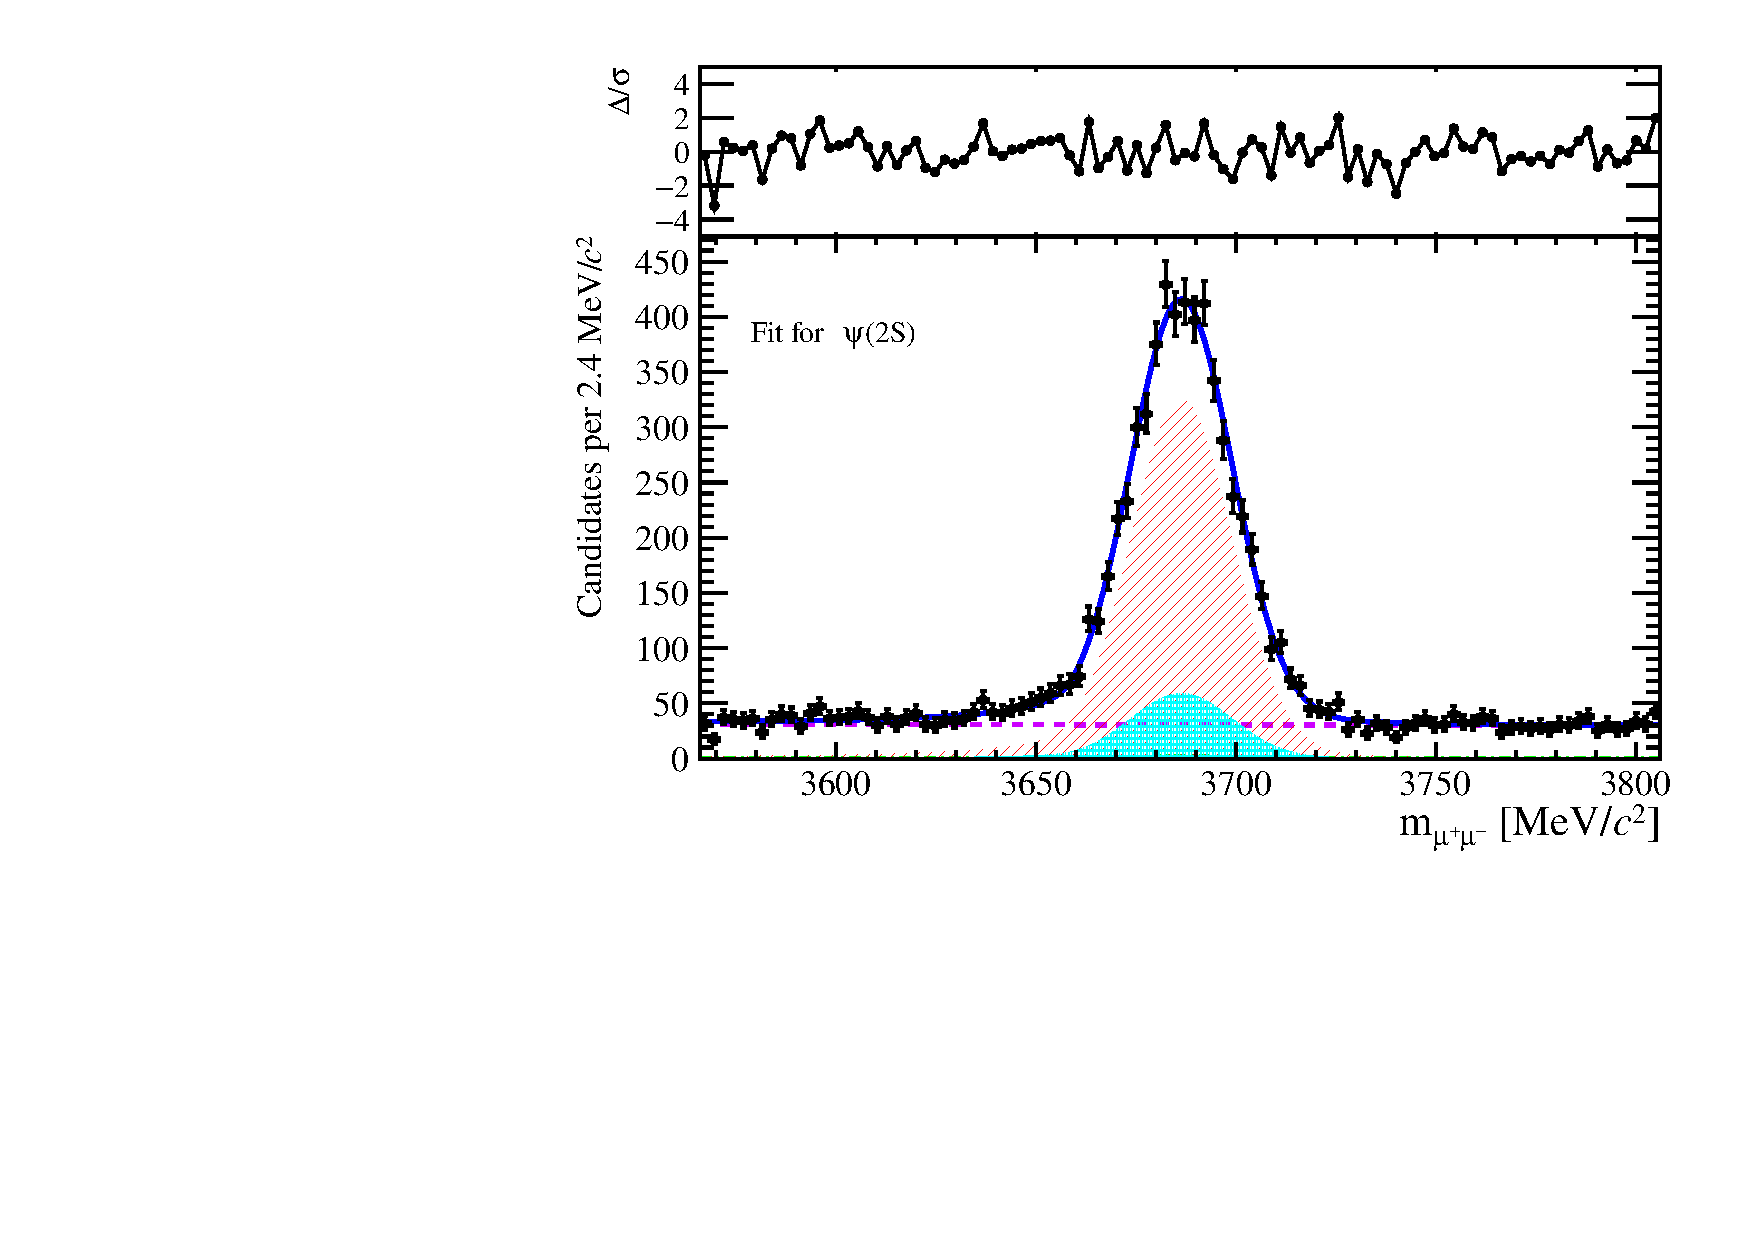
\includegraphics[width=0.47\linewidth]{pdf/Psi2S/drawmassF/n1y1pt2.pdf}
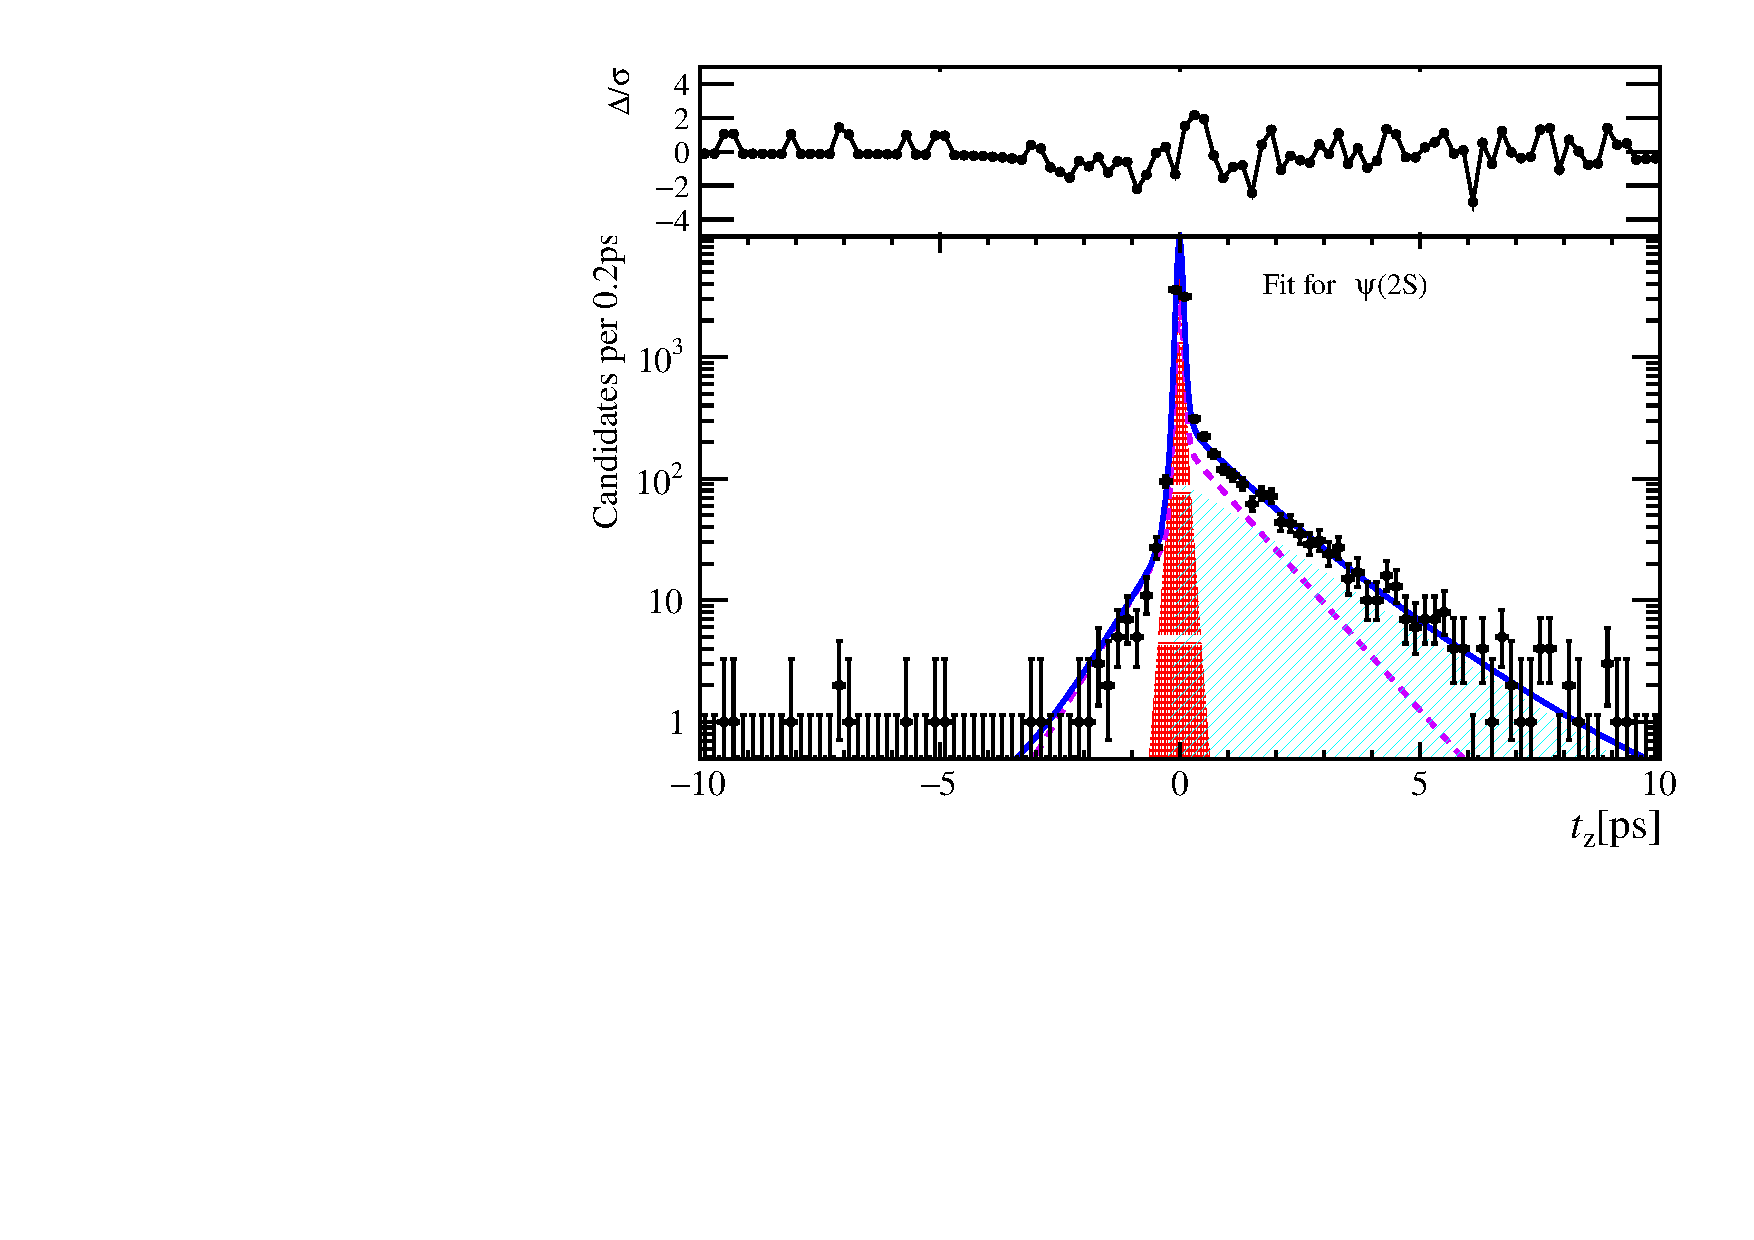
\includegraphics[width=0.47\linewidth]{pdf/Psi2S/2DFitF/n1y1pt2.pdf}
\vspace*{-0.5cm}
\end{center}
\caption{Fit results in $2\gevc<\pt<4\gevc$, $2.0<y<2.8$ and 0$\leq$nForwardTracks$<$12.}
\label{Fitn1y1pt2}
\end{figure}
\begin{figure}[H]
\begin{center}
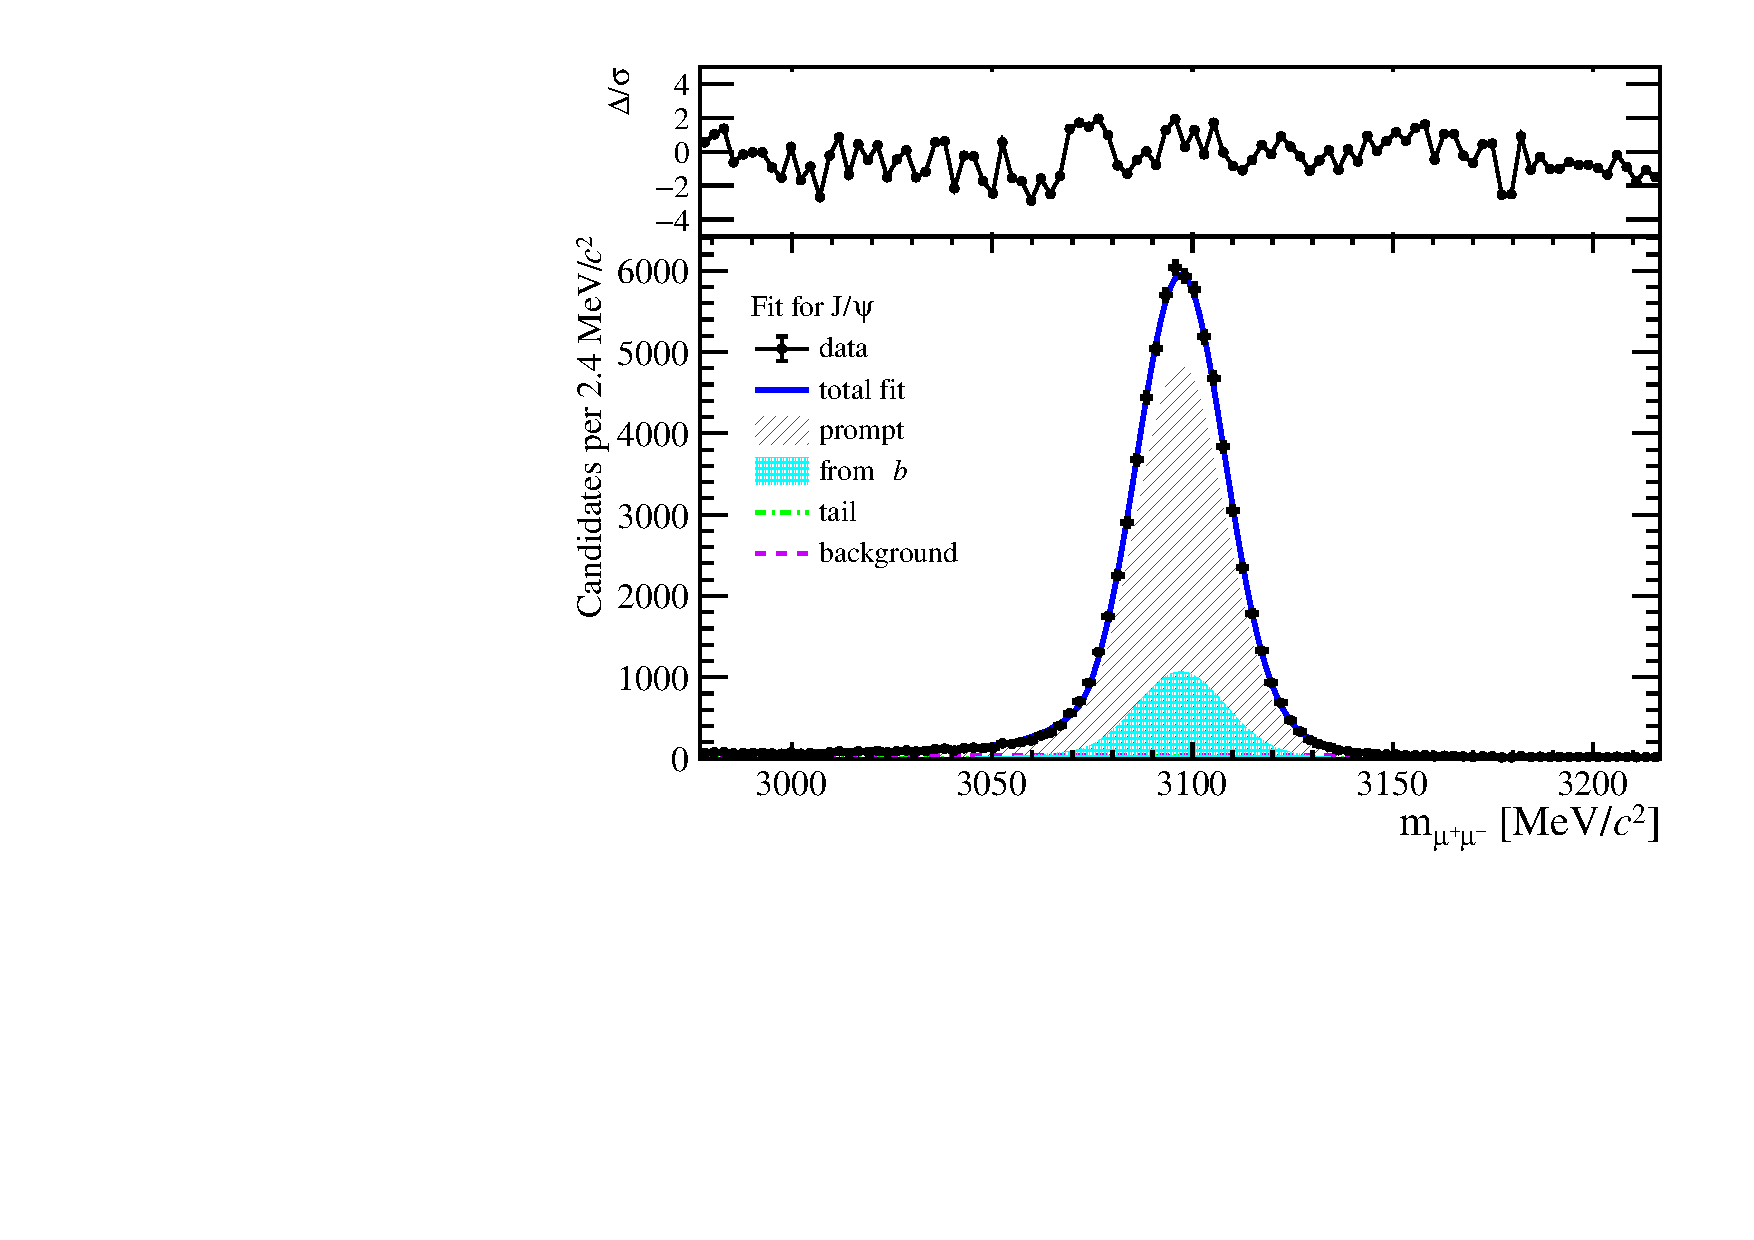
\includegraphics[width=0.47\linewidth]{pdf/Jpsi/drawmassF/n1y1pt3.pdf}
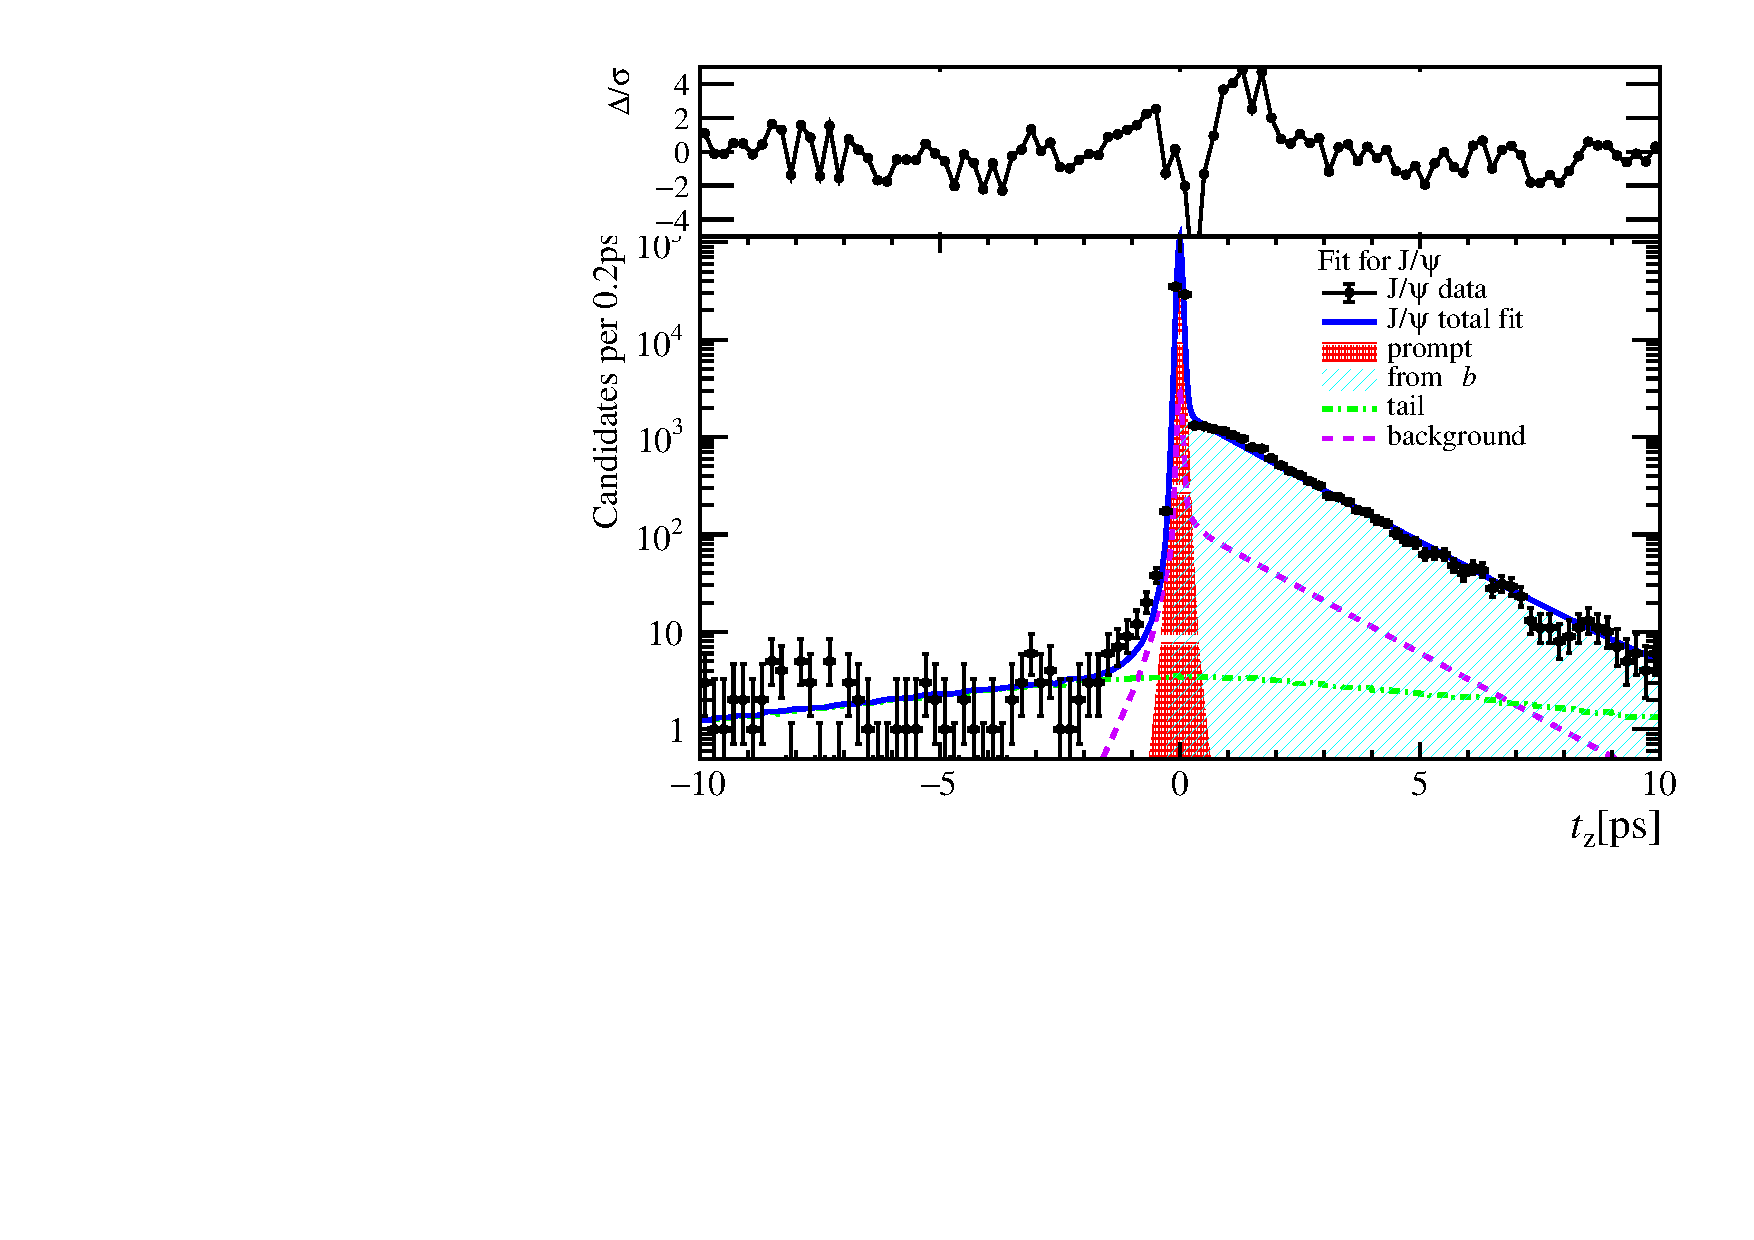
\includegraphics[width=0.47\linewidth]{pdf/Jpsi/2DFitF/n1y1pt3.pdf}
\vspace*{-0.5cm}
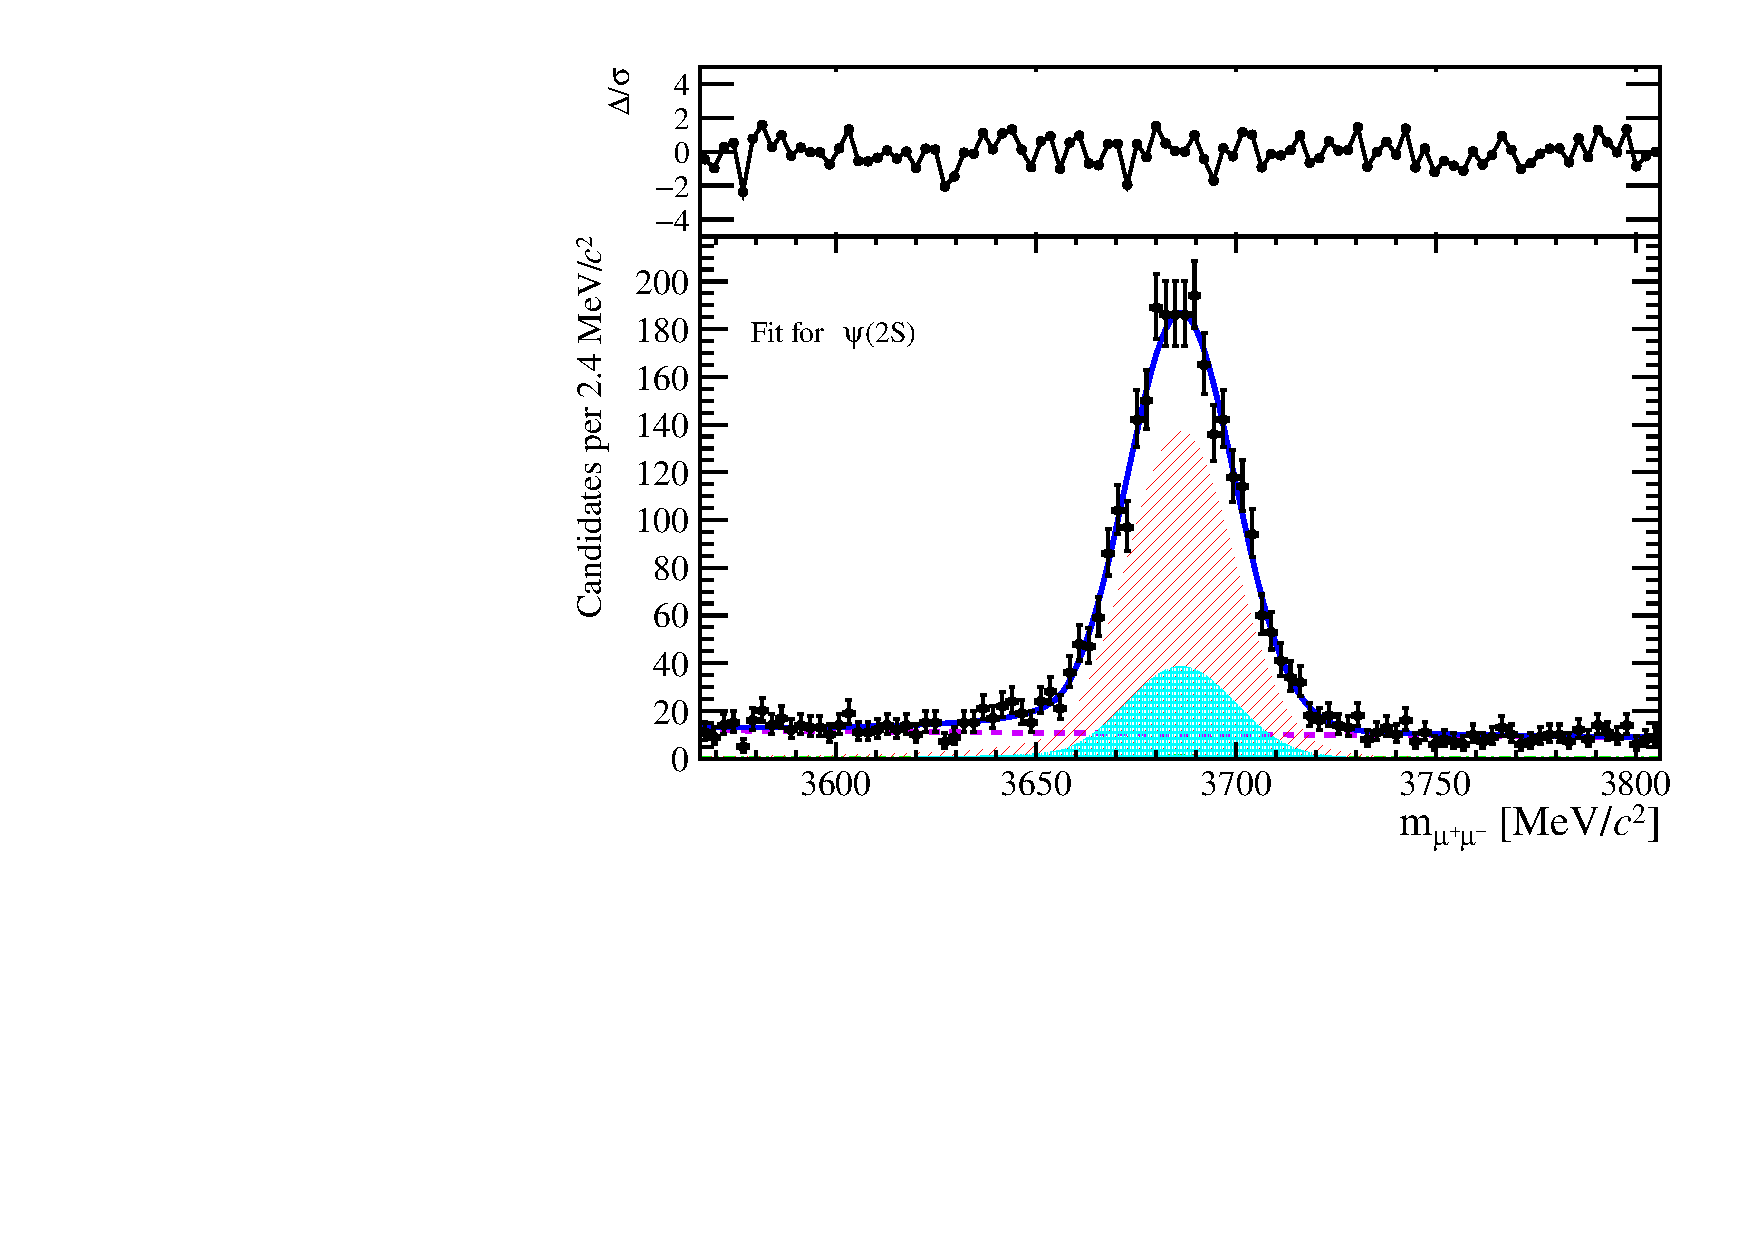
\includegraphics[width=0.47\linewidth]{pdf/Psi2S/drawmassF/n1y1pt3.pdf}
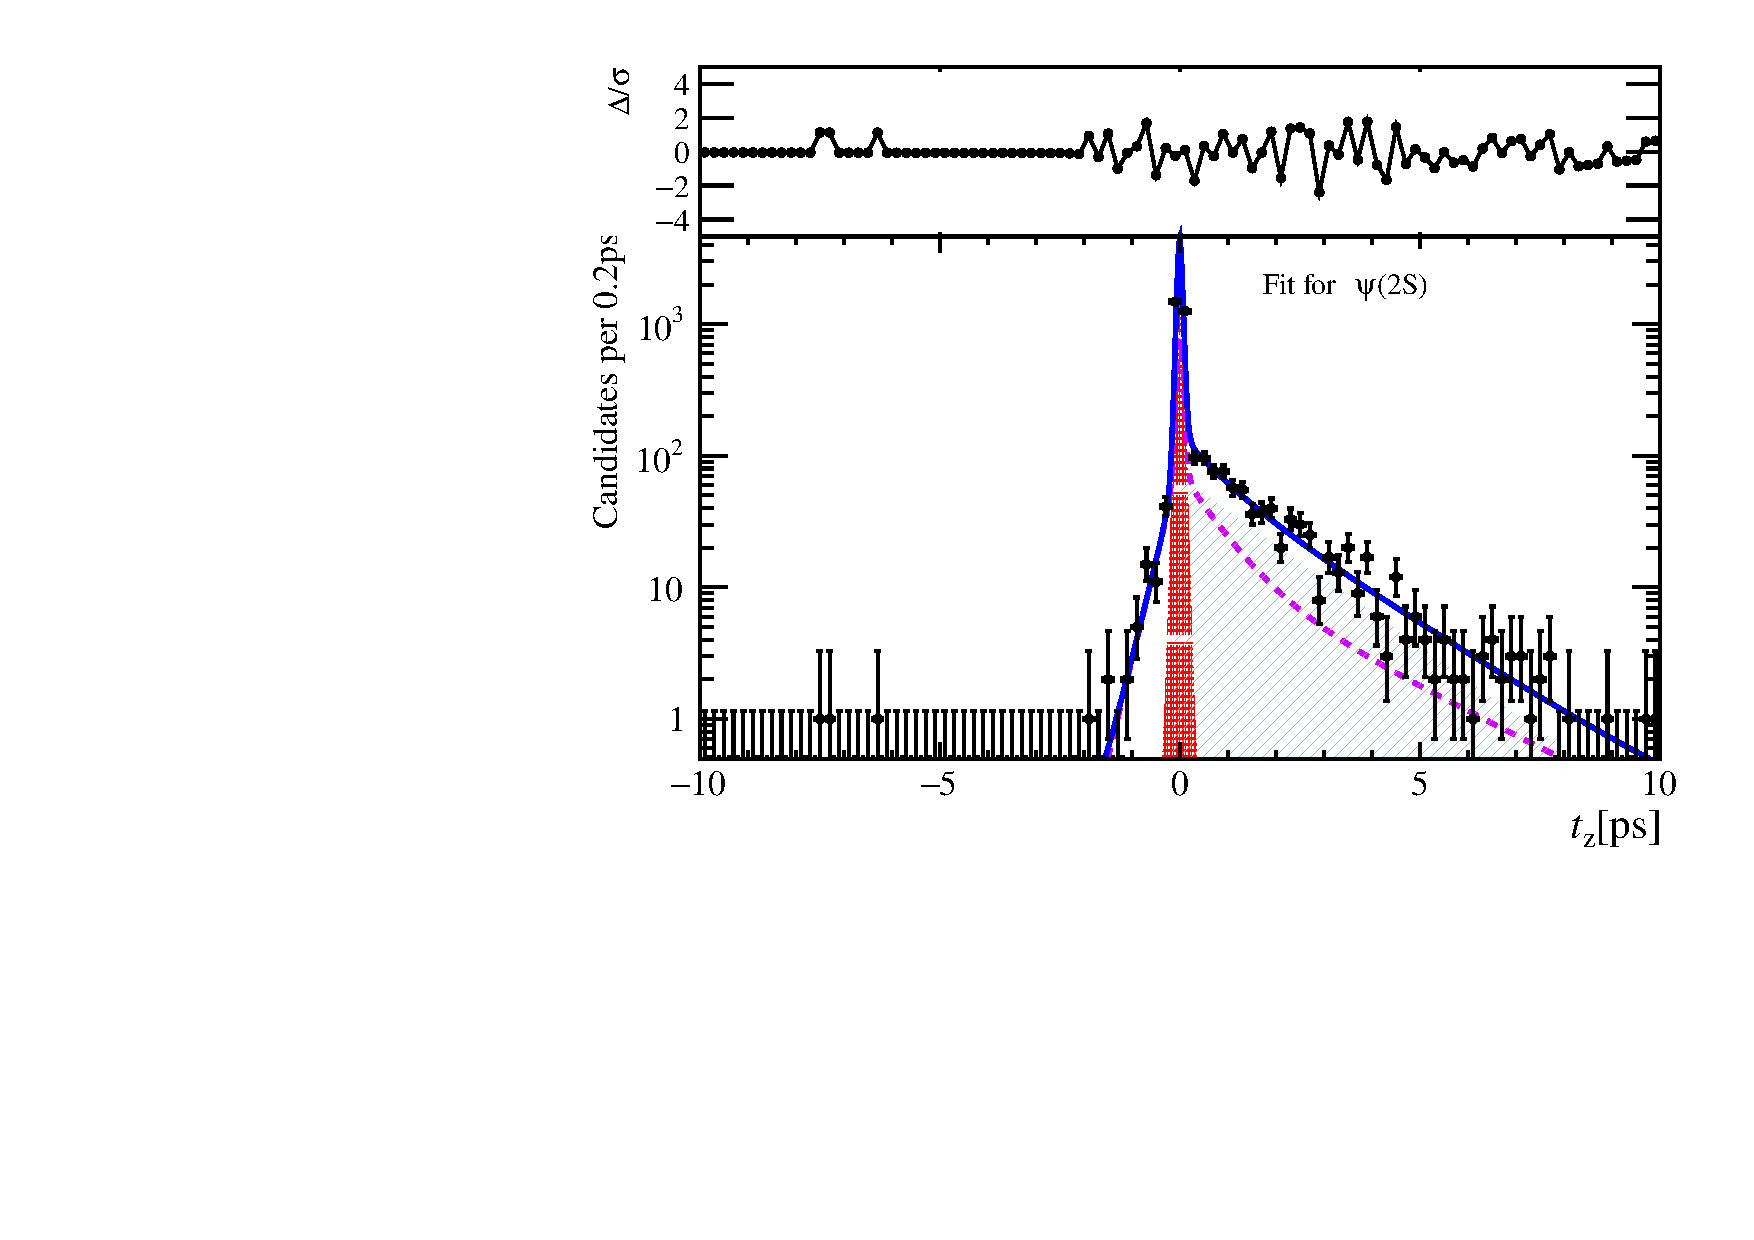
\includegraphics[width=0.47\linewidth]{pdf/Psi2S/2DFitF/n1y1pt3.pdf}
\vspace*{-0.5cm}
\end{center}
\caption{Fit results in $4\gevc<\pt<6\gevc$, $2.0<y<2.8$ and 0$\leq$nForwardTracks$<$12.}
\label{Fitn1y1pt3}
\end{figure}
\begin{figure}[H]
\begin{center}
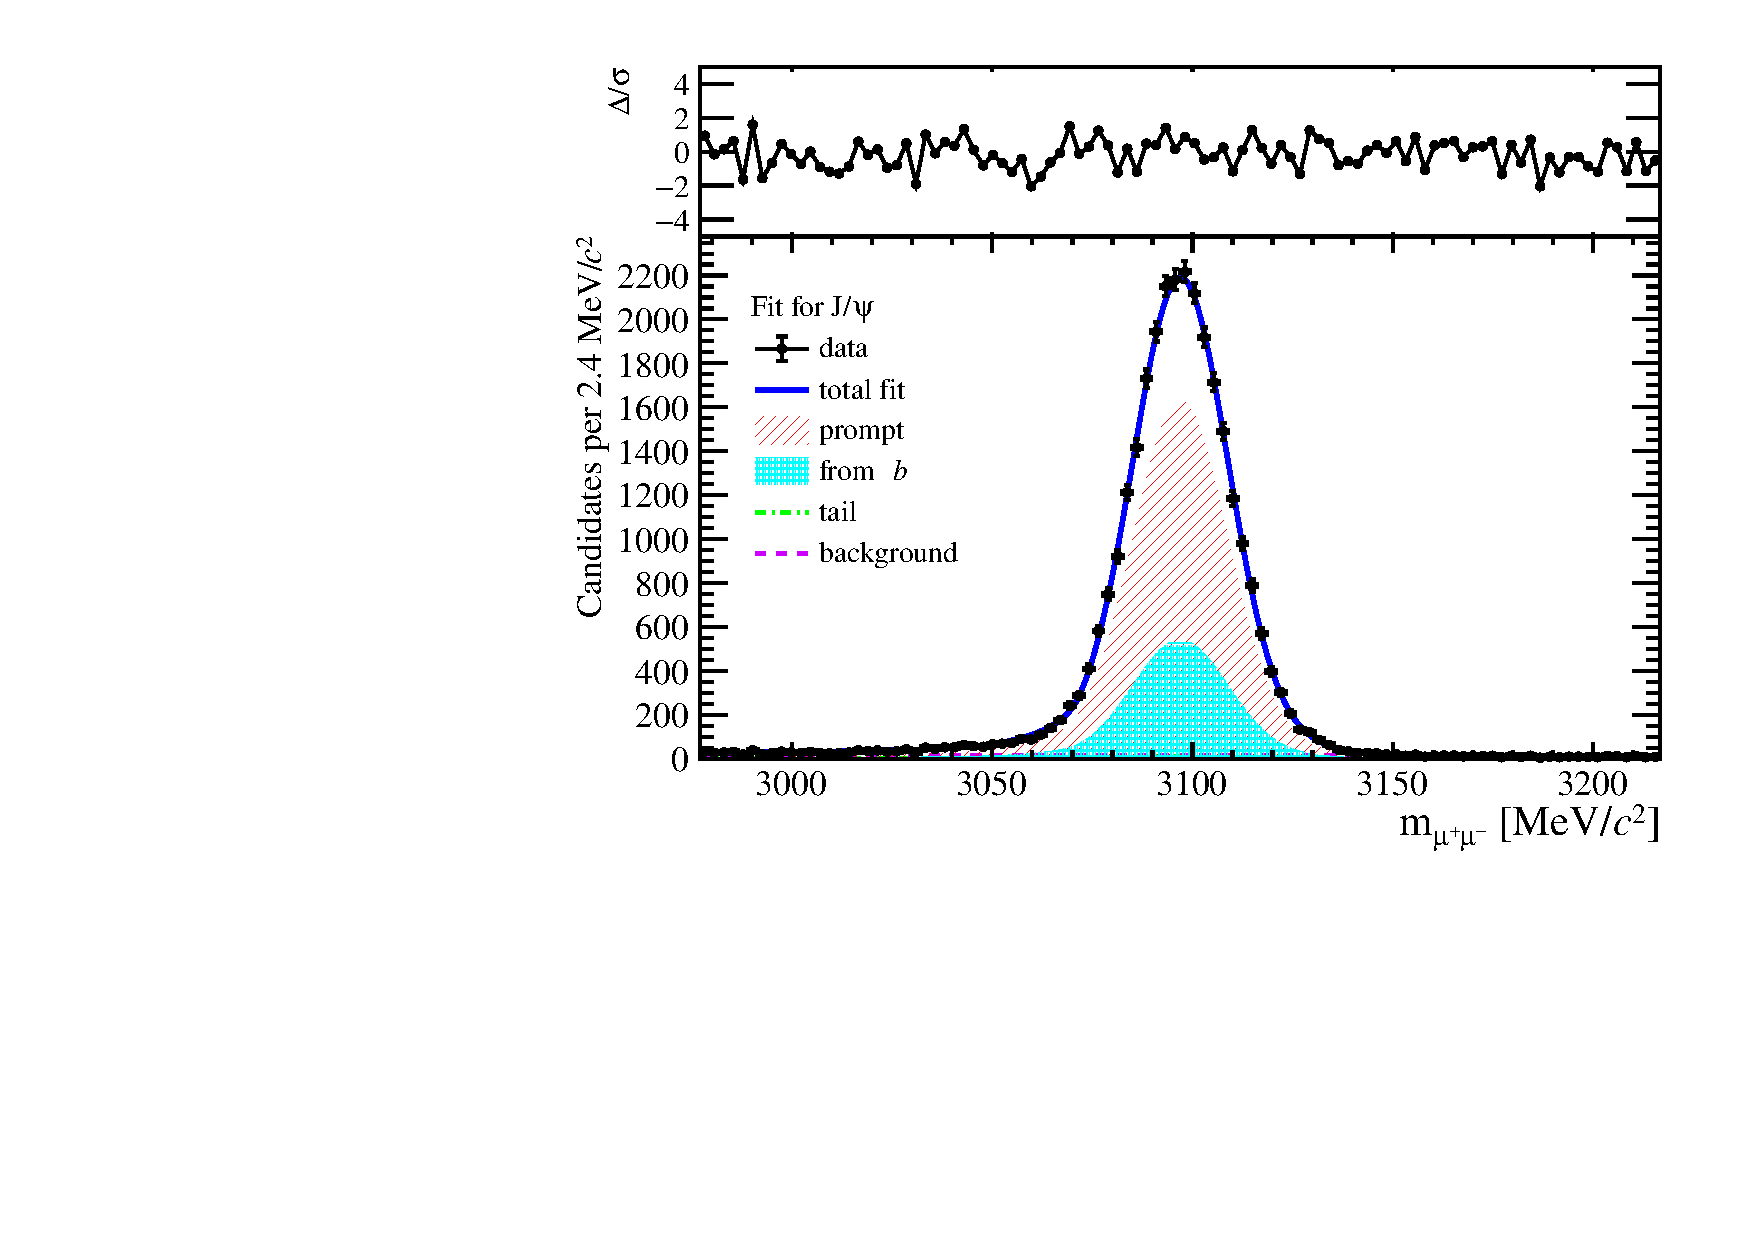
\includegraphics[width=0.47\linewidth]{pdf/Jpsi/drawmassF/n1y1pt4.pdf}
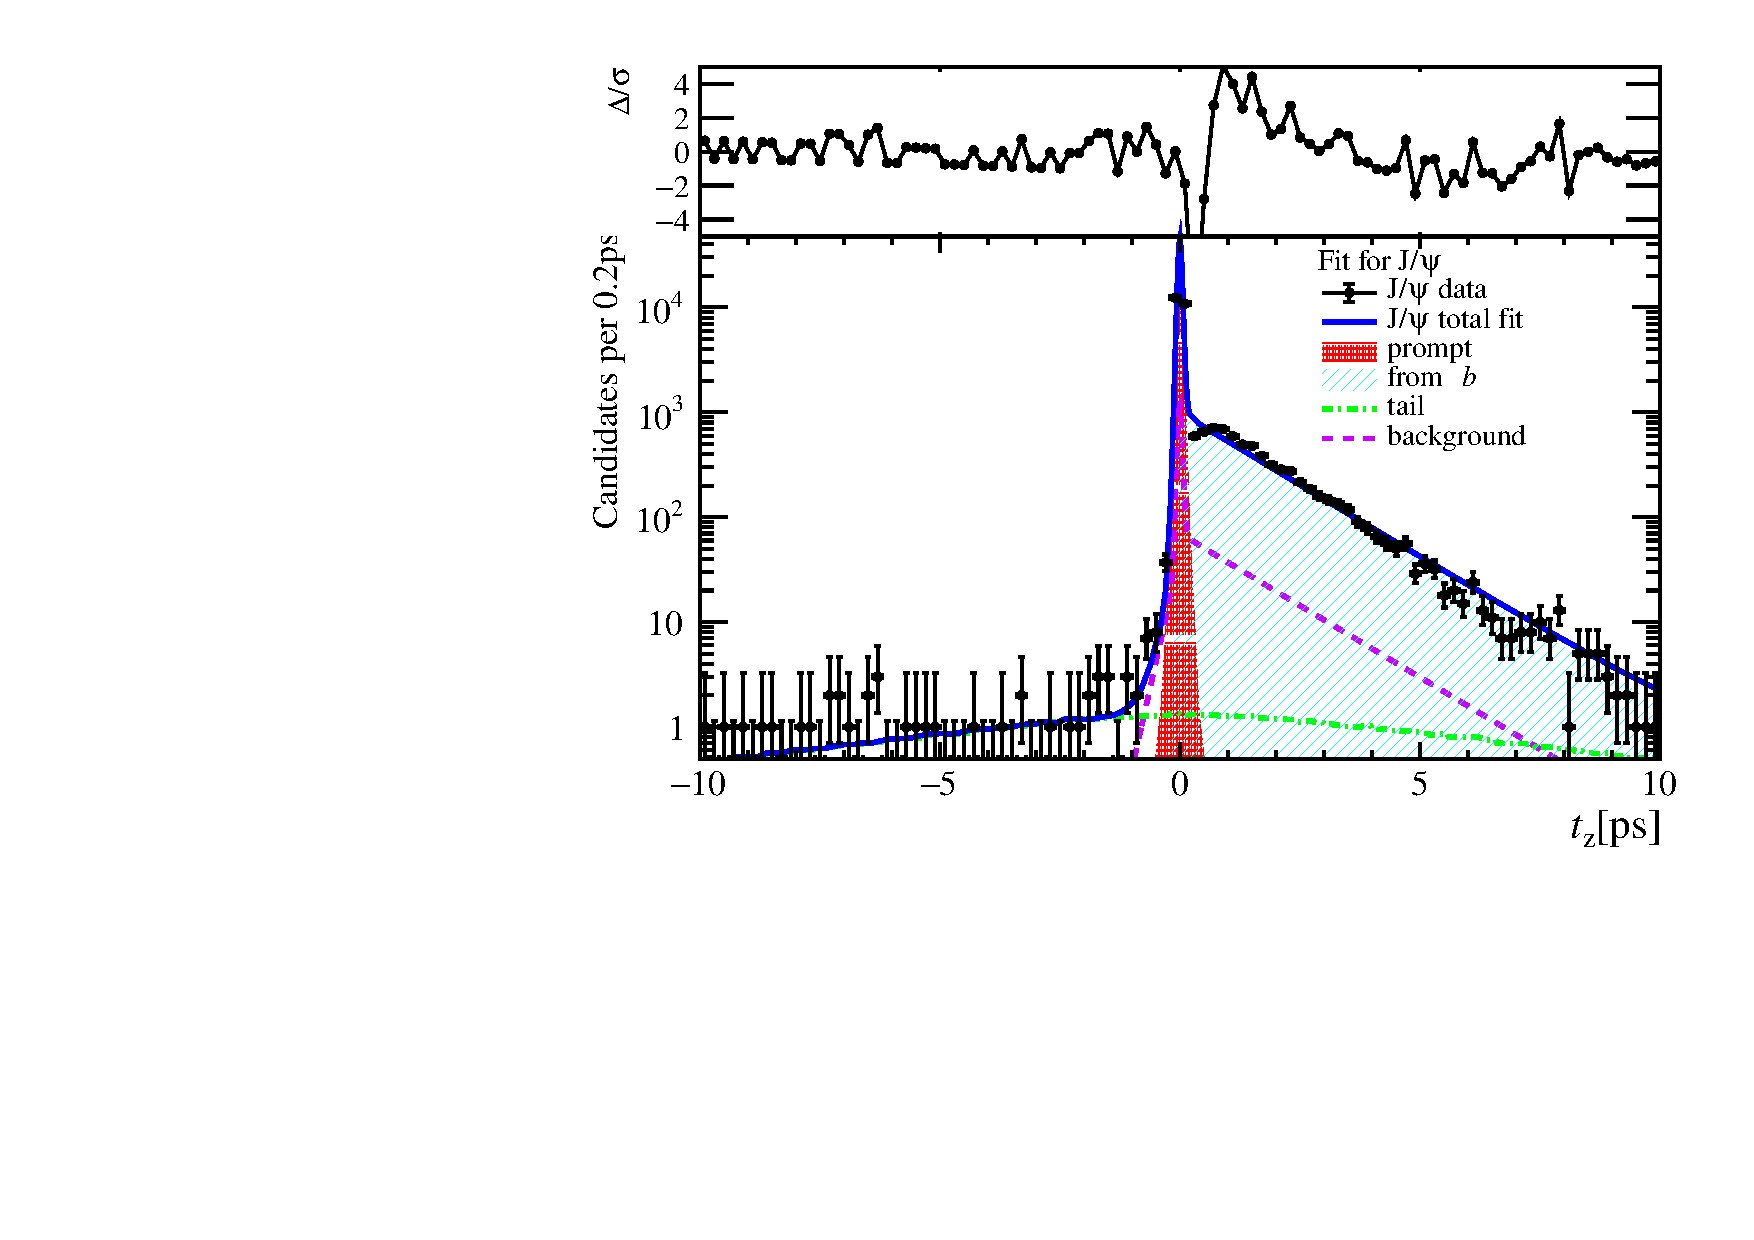
\includegraphics[width=0.47\linewidth]{pdf/Jpsi/2DFitF/n1y1pt4.pdf}
\vspace*{-0.5cm}
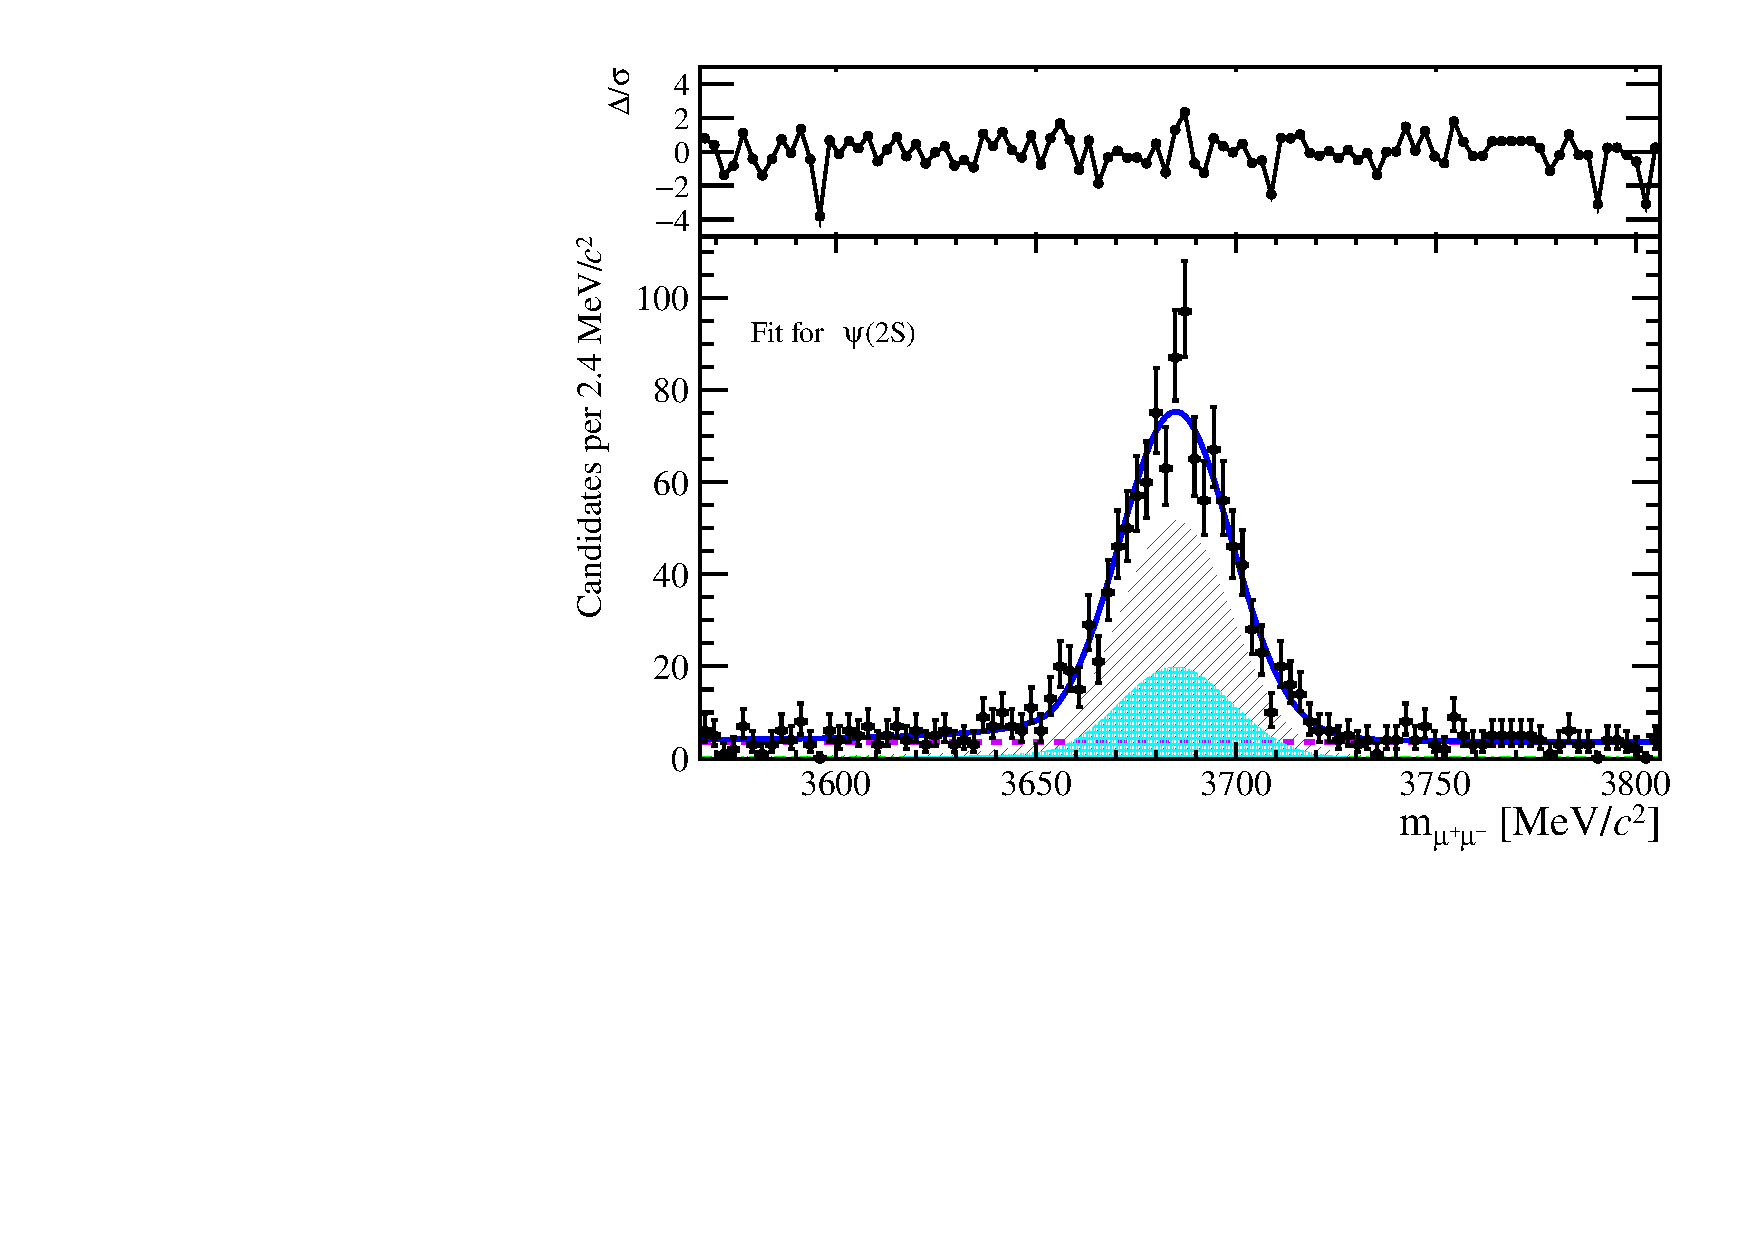
\includegraphics[width=0.47\linewidth]{pdf/Psi2S/drawmassF/n1y1pt4.pdf}
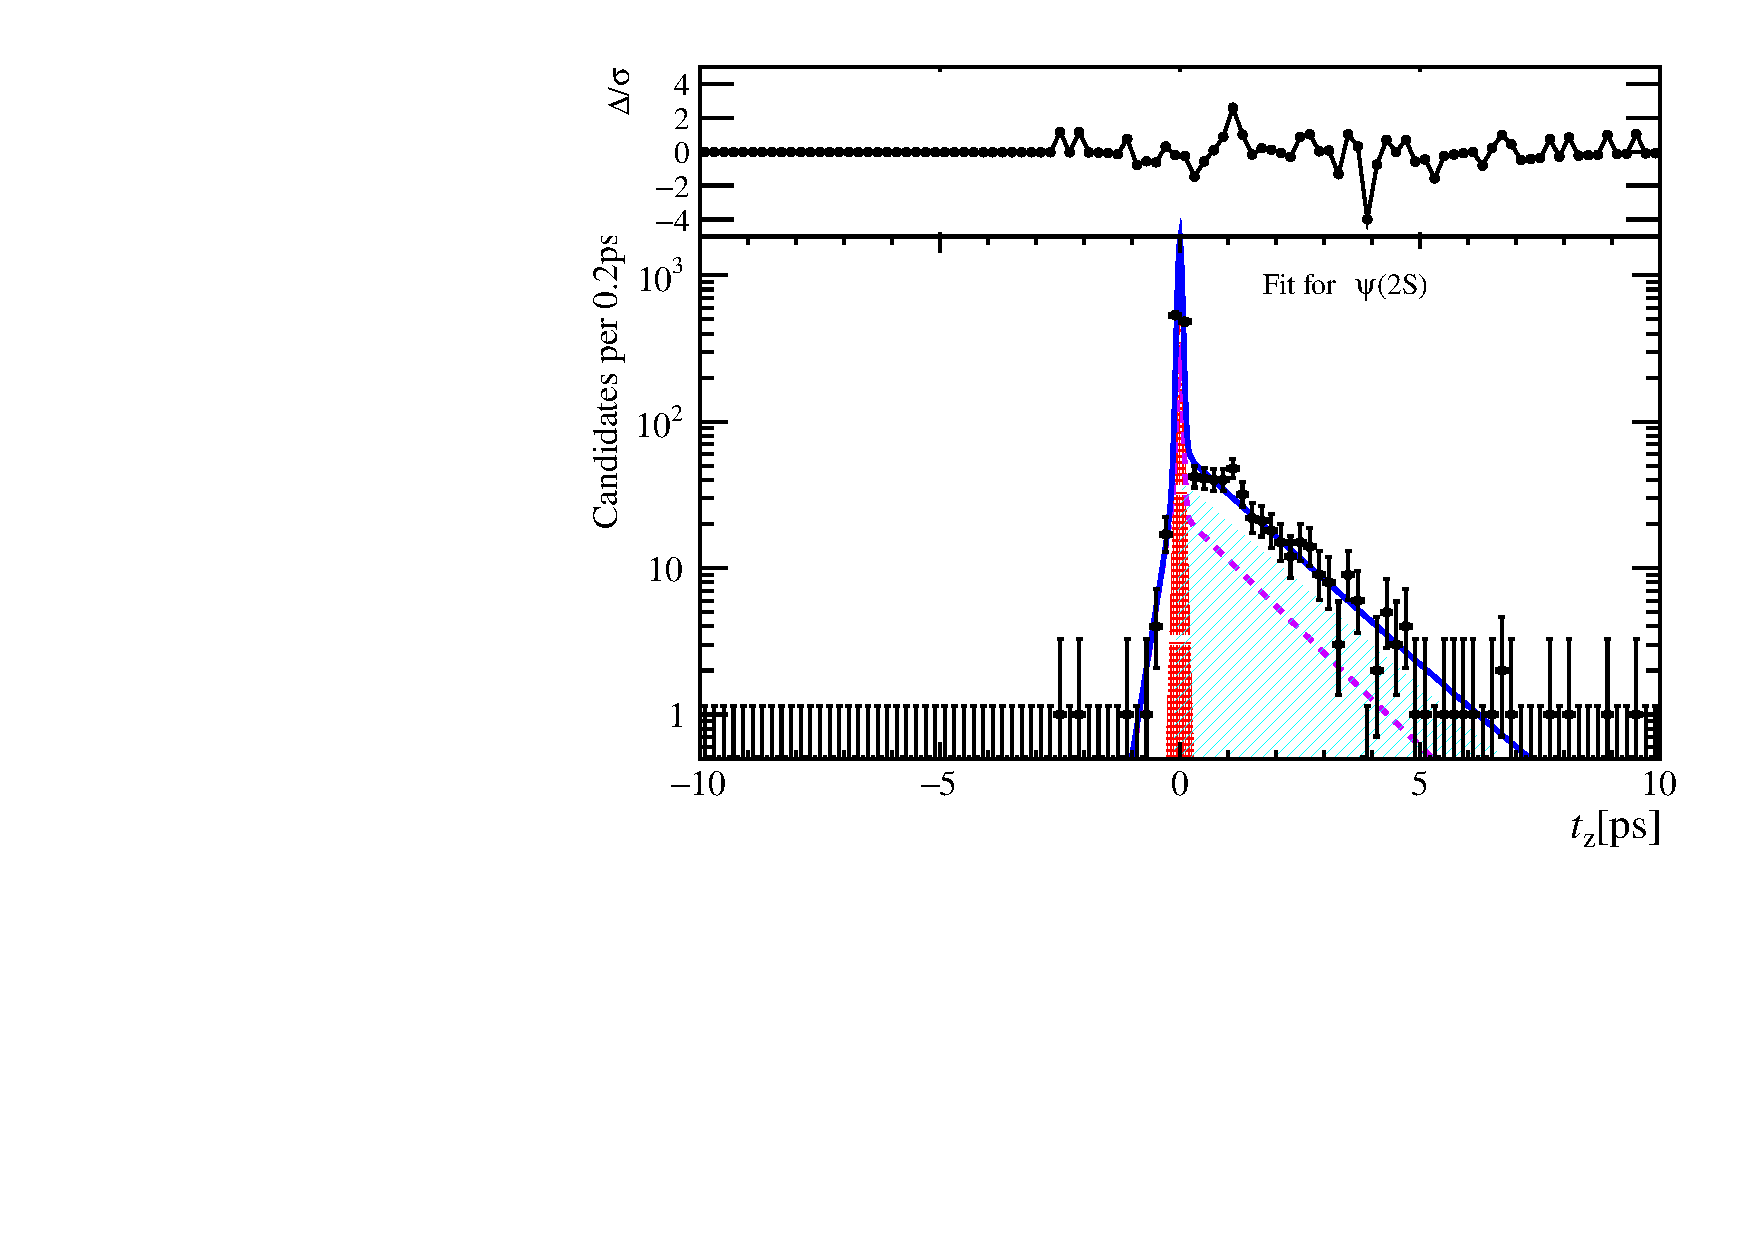
\includegraphics[width=0.47\linewidth]{pdf/Psi2S/2DFitF/n1y1pt4.pdf}
\vspace*{-0.5cm}
\end{center}
\caption{Fit results in $6\gevc<\pt<8\gevc$, $2.0<y<2.8$ and 0$\leq$nForwardTracks$<$12.}
\label{Fitn1y1pt4}
\end{figure}
\begin{figure}[H]
\begin{center}
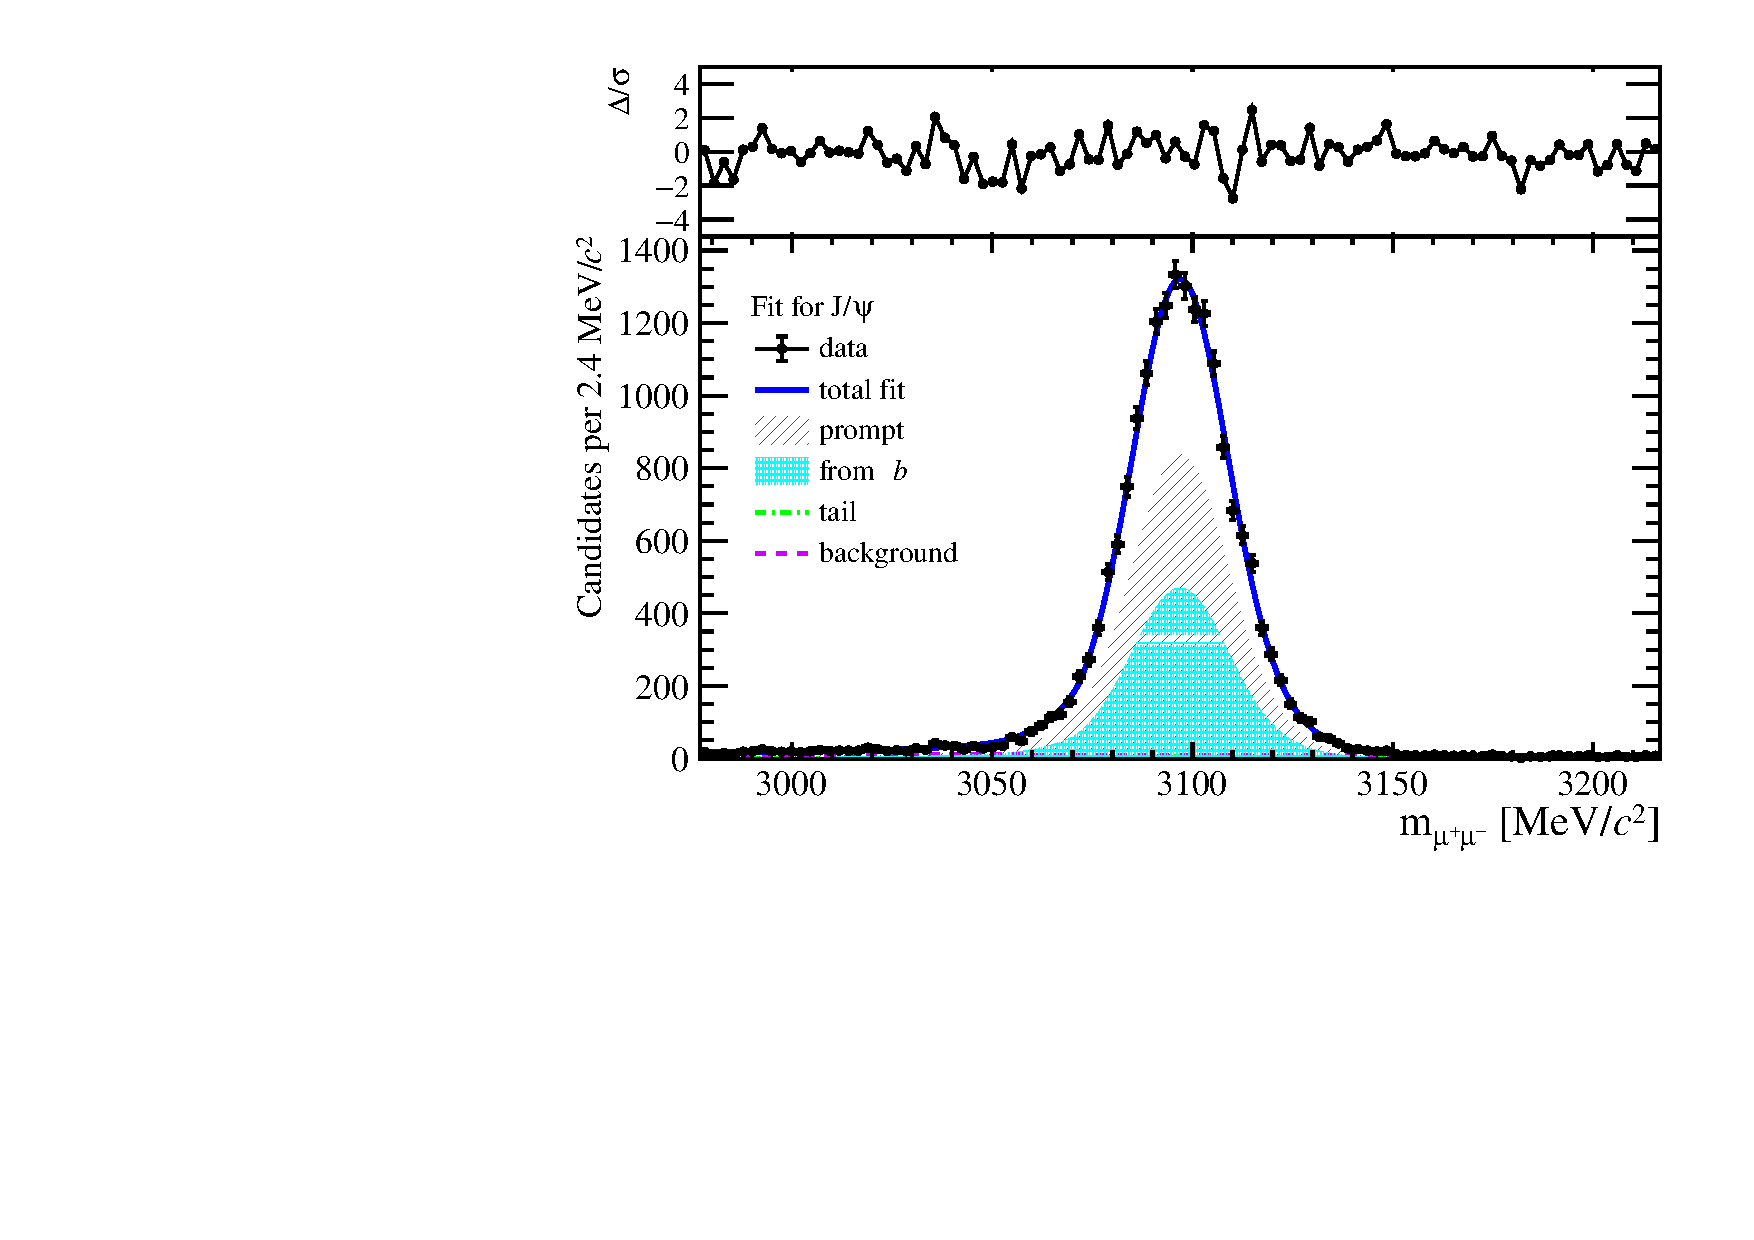
\includegraphics[width=0.47\linewidth]{pdf/Jpsi/drawmassF/n1y1pt5.pdf}
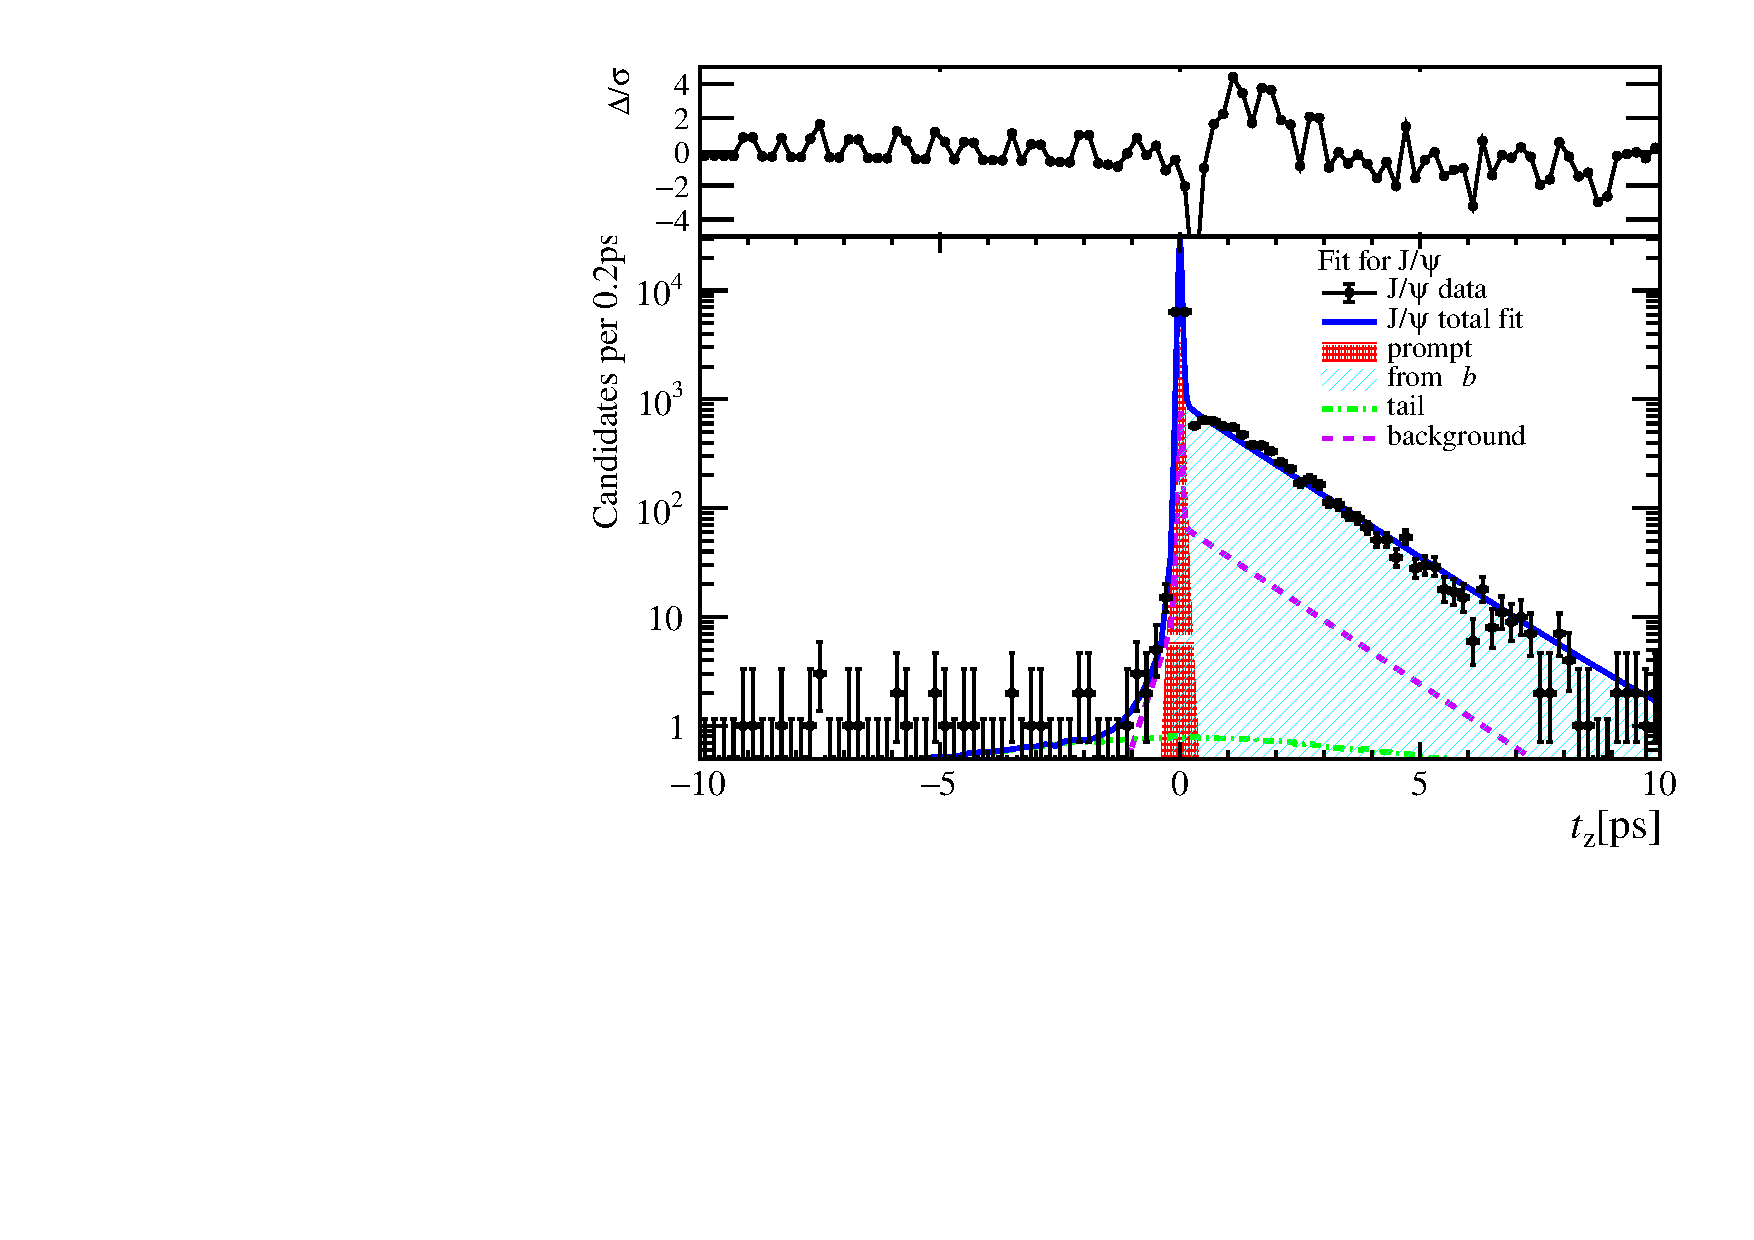
\includegraphics[width=0.47\linewidth]{pdf/Jpsi/2DFitF/n1y1pt5.pdf}
\vspace*{-0.5cm}
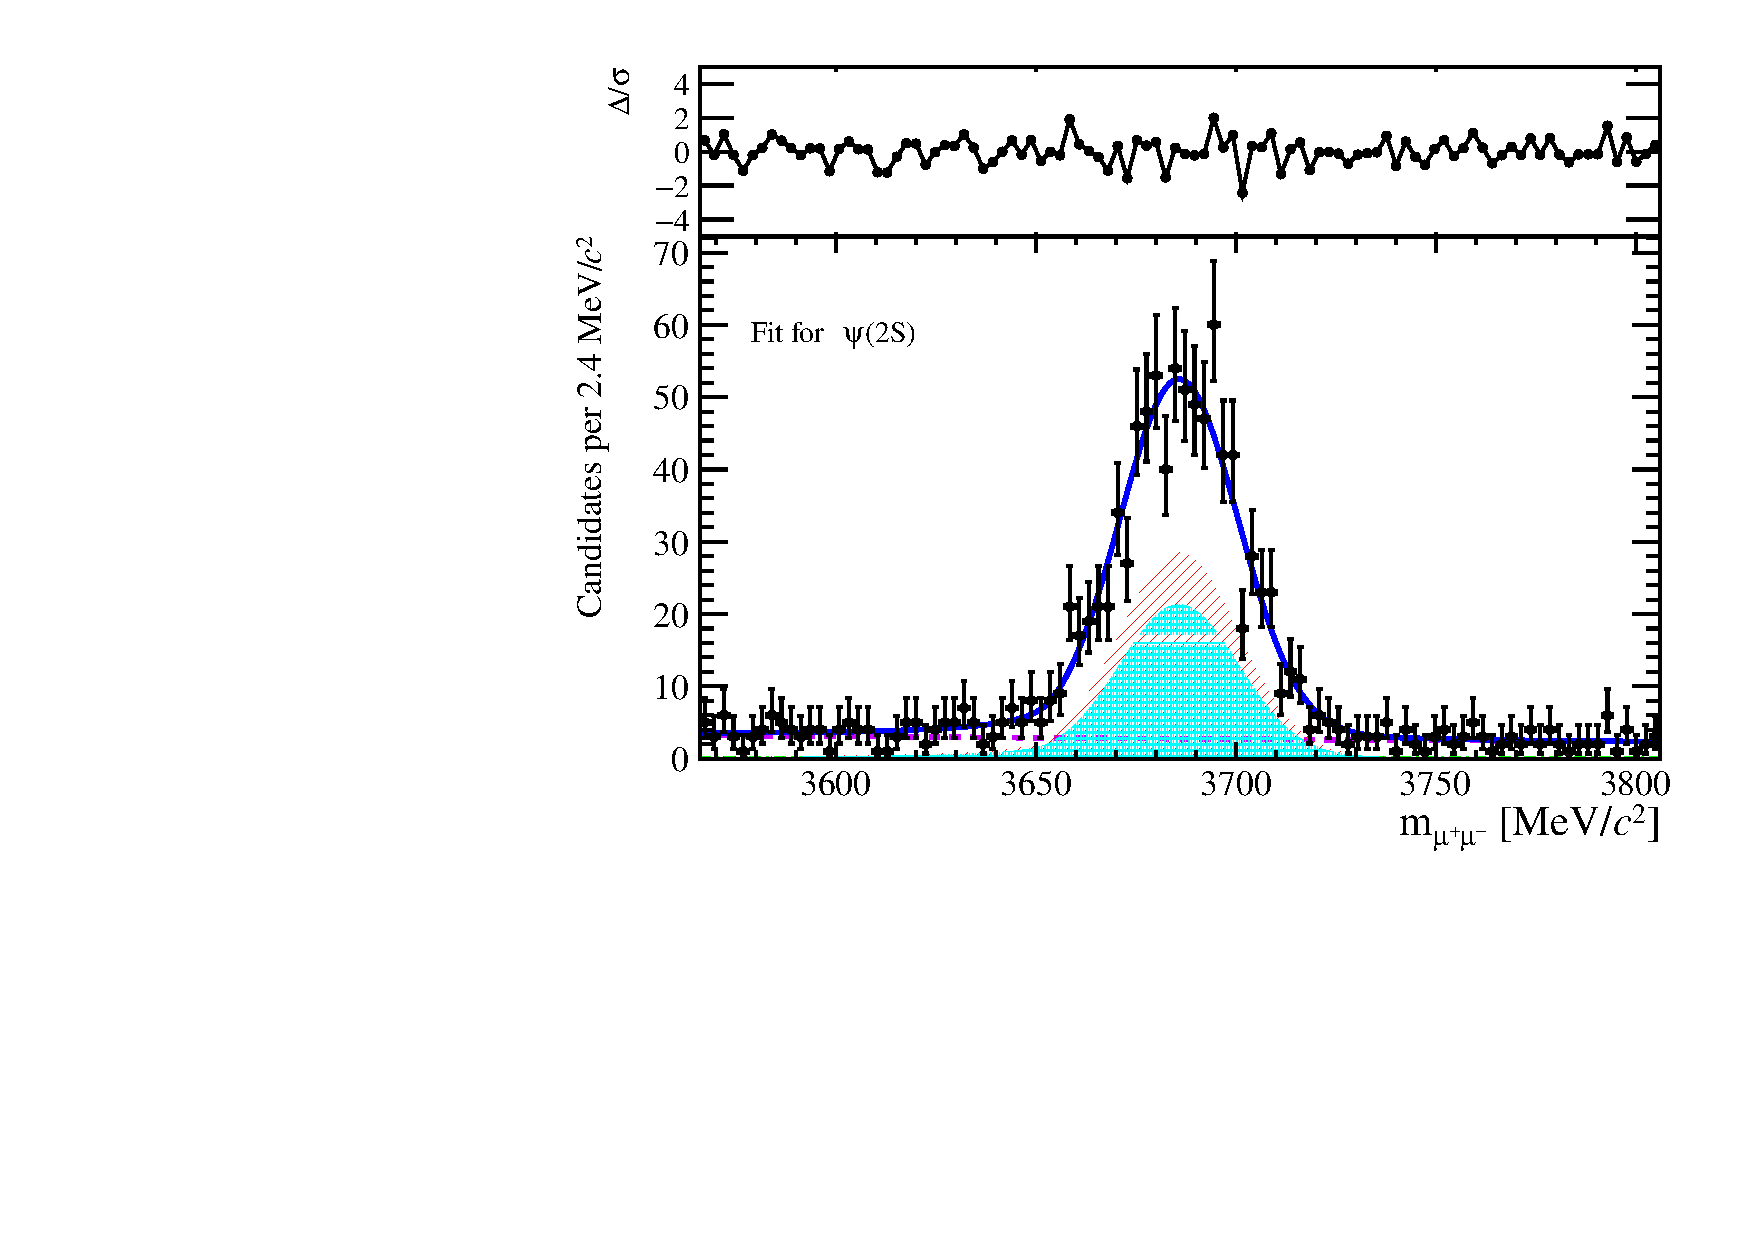
\includegraphics[width=0.47\linewidth]{pdf/Psi2S/drawmassF/n1y1pt5.pdf}
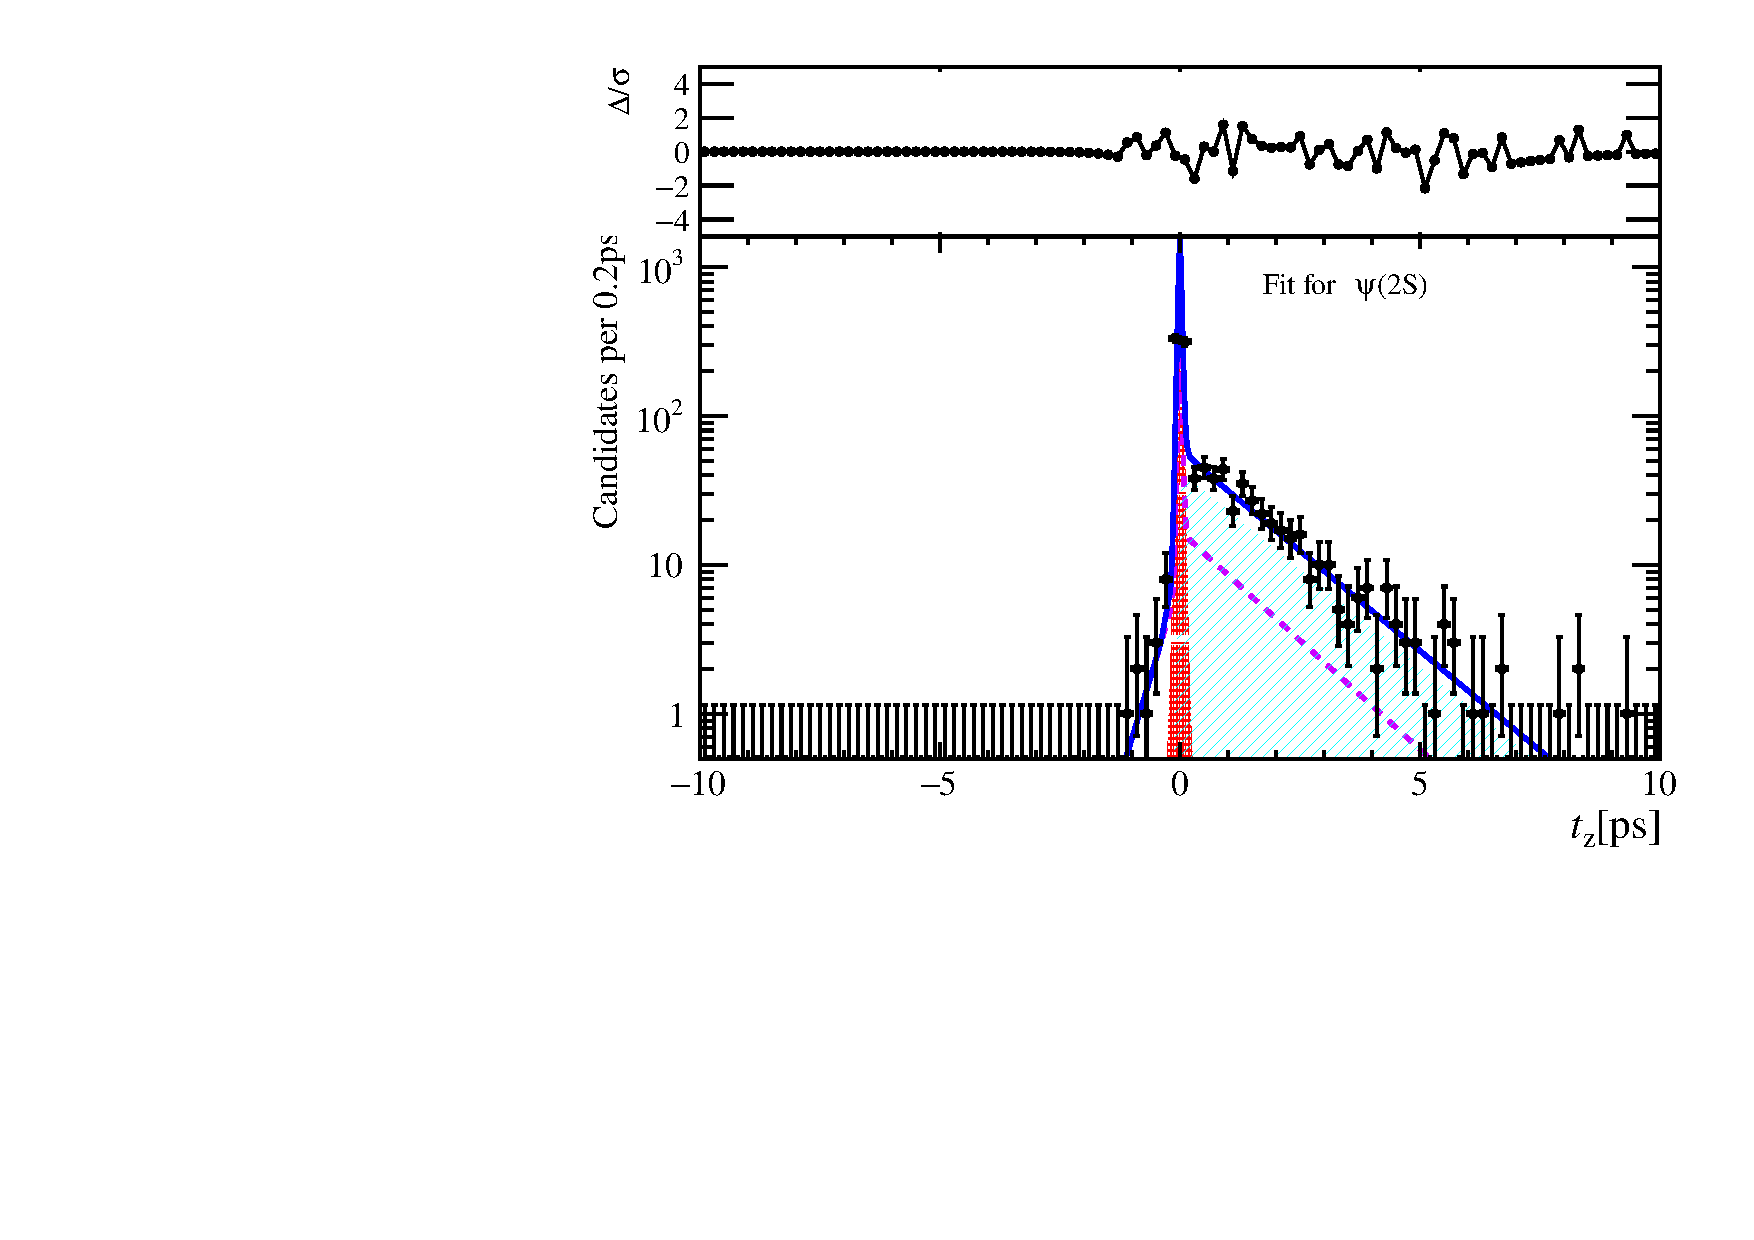
\includegraphics[width=0.47\linewidth]{pdf/Psi2S/2DFitF/n1y1pt5.pdf}
\vspace*{-0.5cm}
\end{center}
\caption{Fit results in $8\gevc<\pt<20\gevc$, $2.0<y<2.8$ and 0$\leq$nForwardTracks$<$12.}
\label{Fitn1y1pt5}
\end{figure}
\begin{figure}[H]
\begin{center}
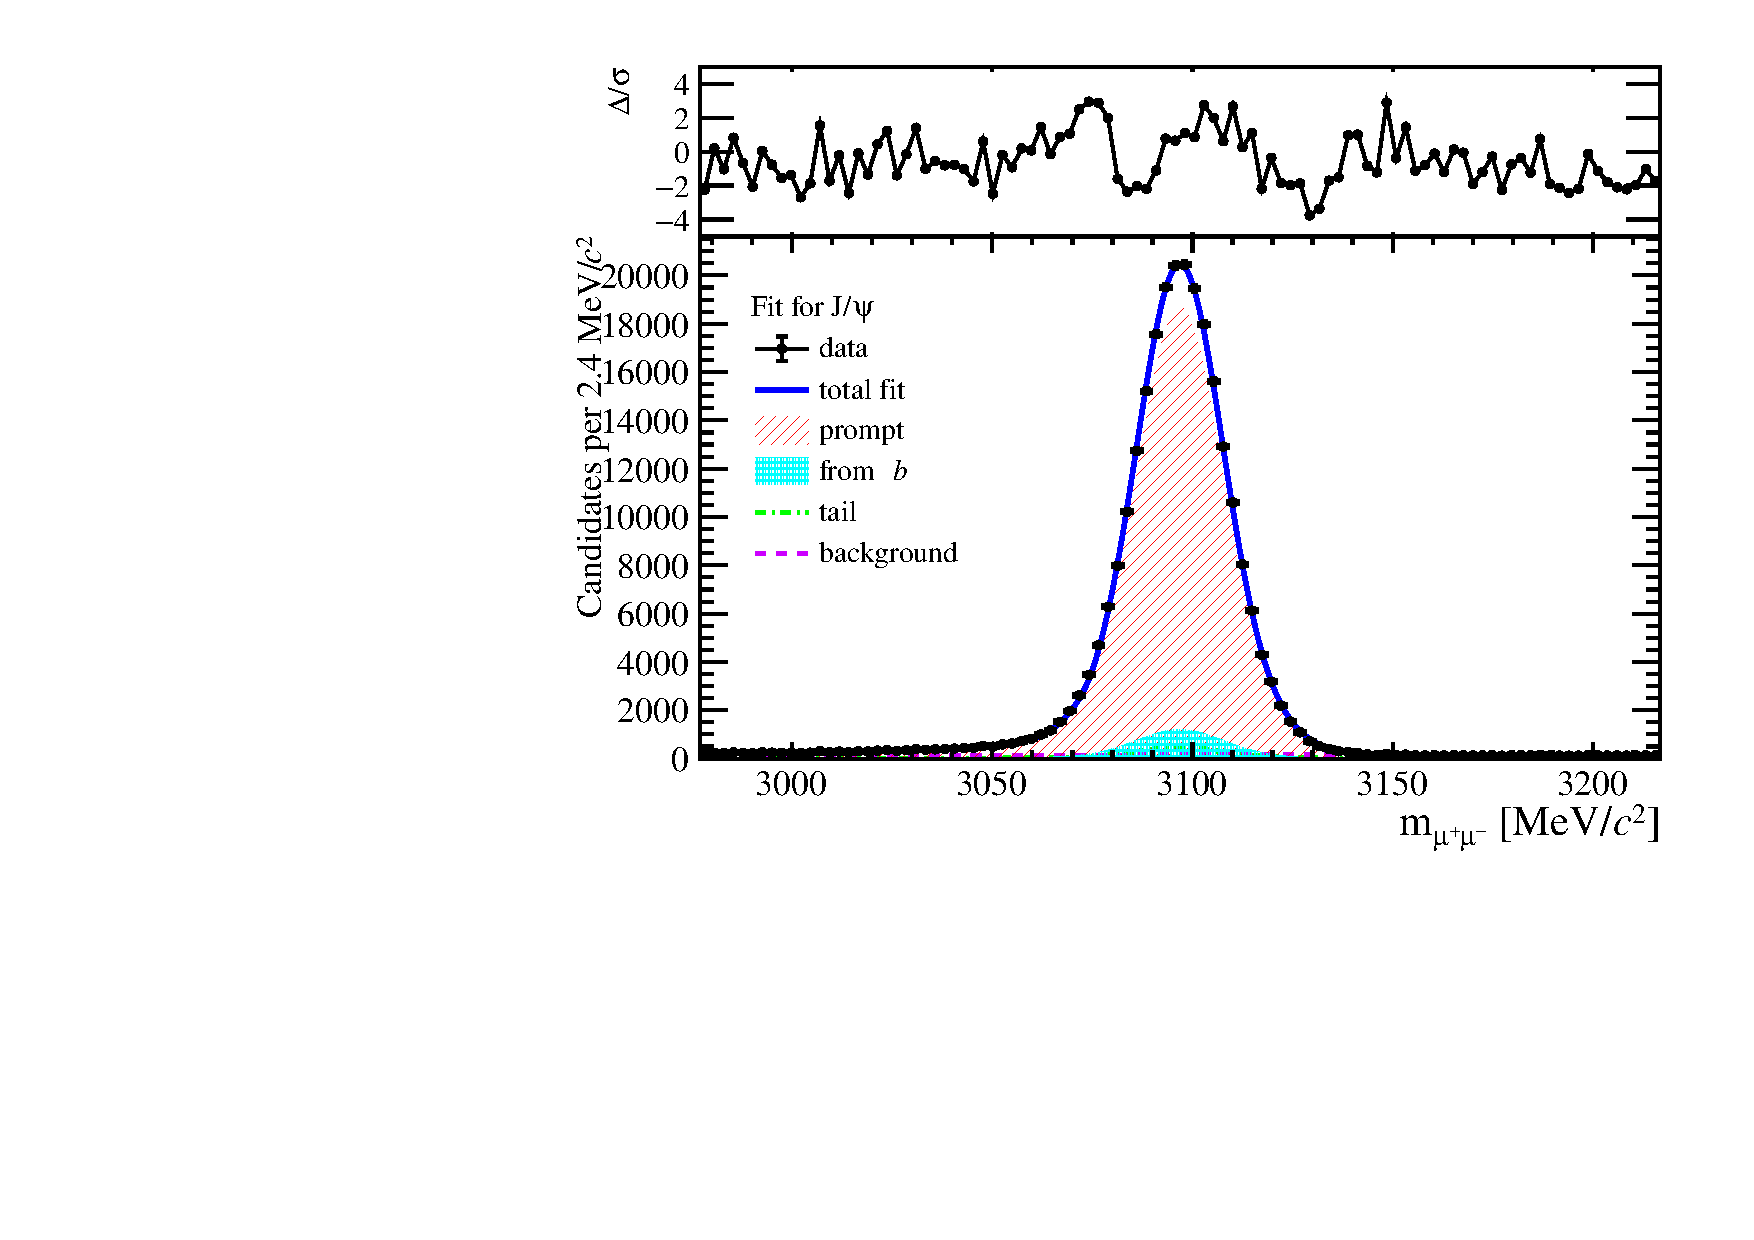
\includegraphics[width=0.47\linewidth]{pdf/Jpsi/drawmassF/n1y2pt1.pdf}
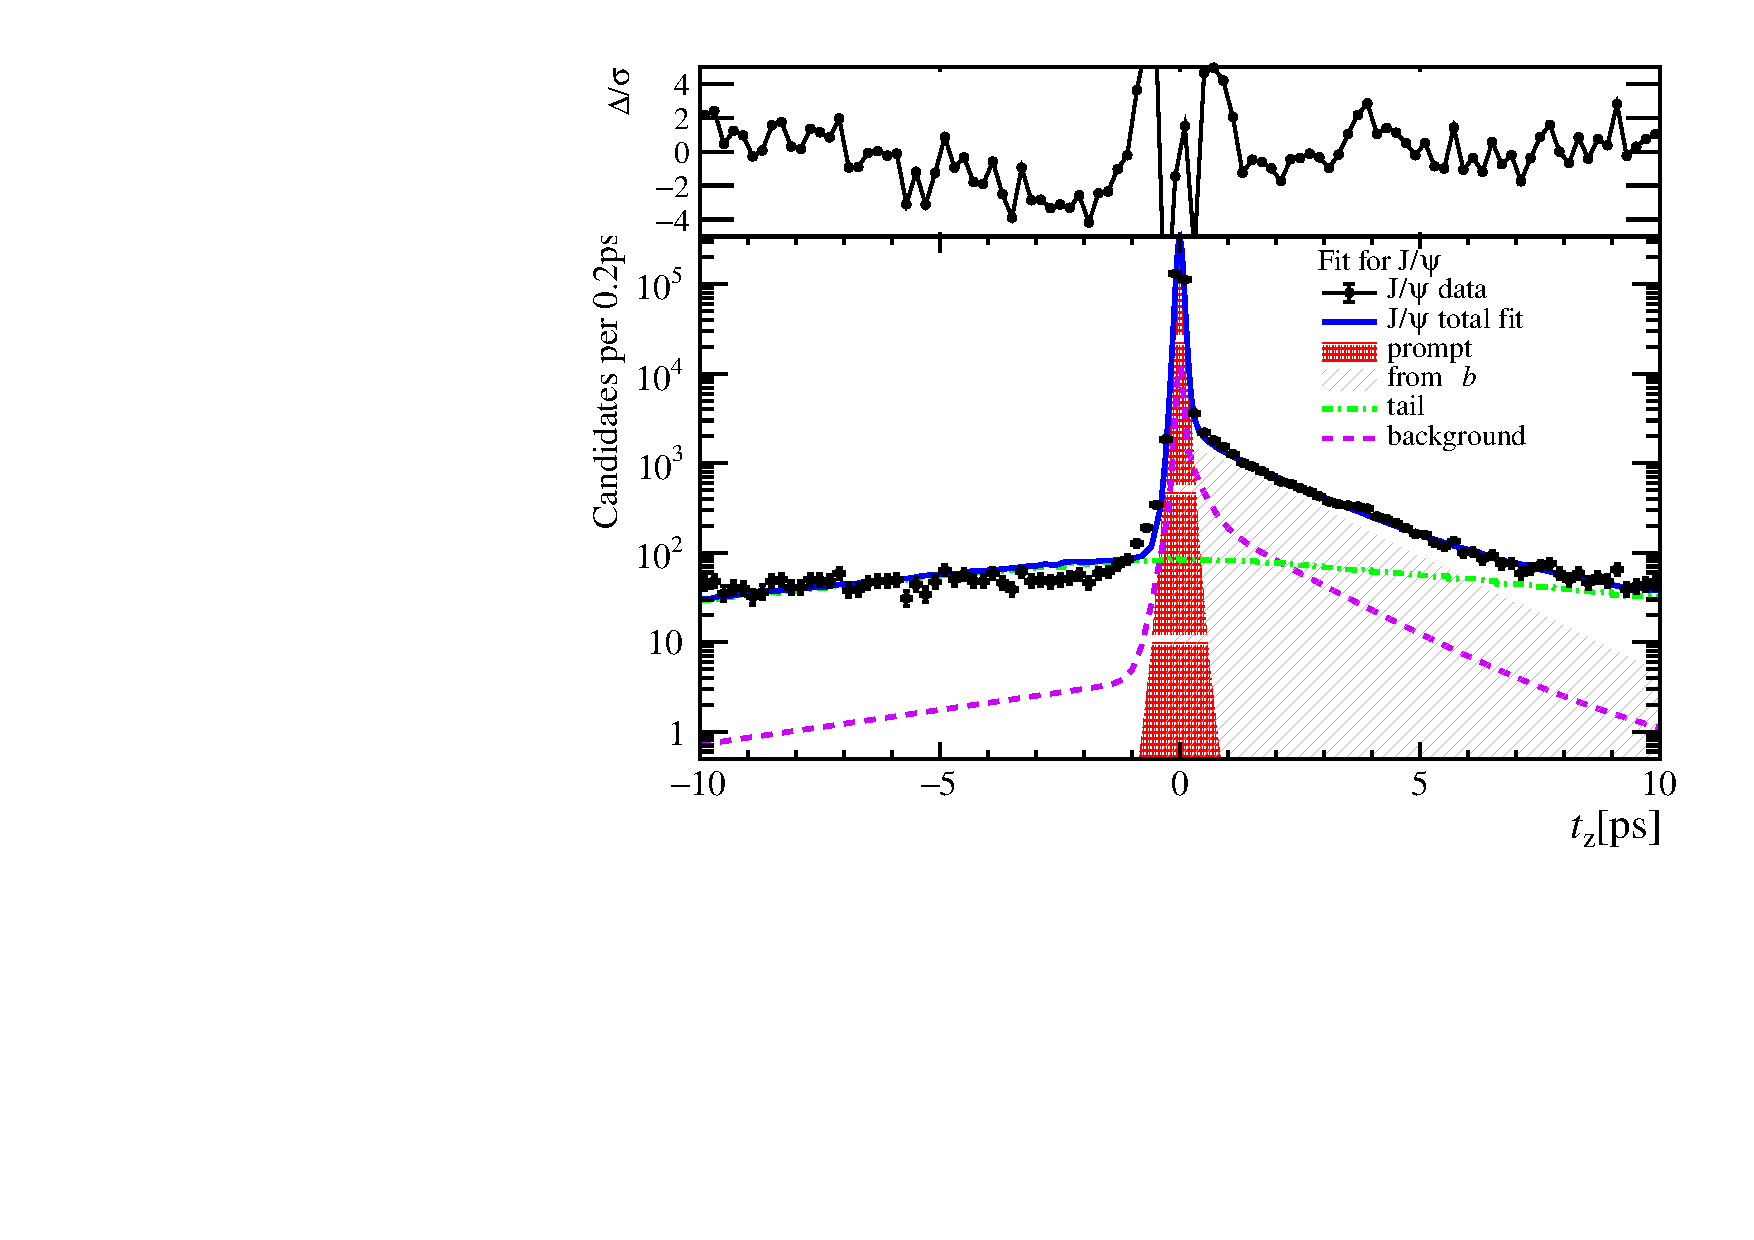
\includegraphics[width=0.47\linewidth]{pdf/Jpsi/2DFitF/n1y2pt1.pdf}
\vspace*{-0.5cm}
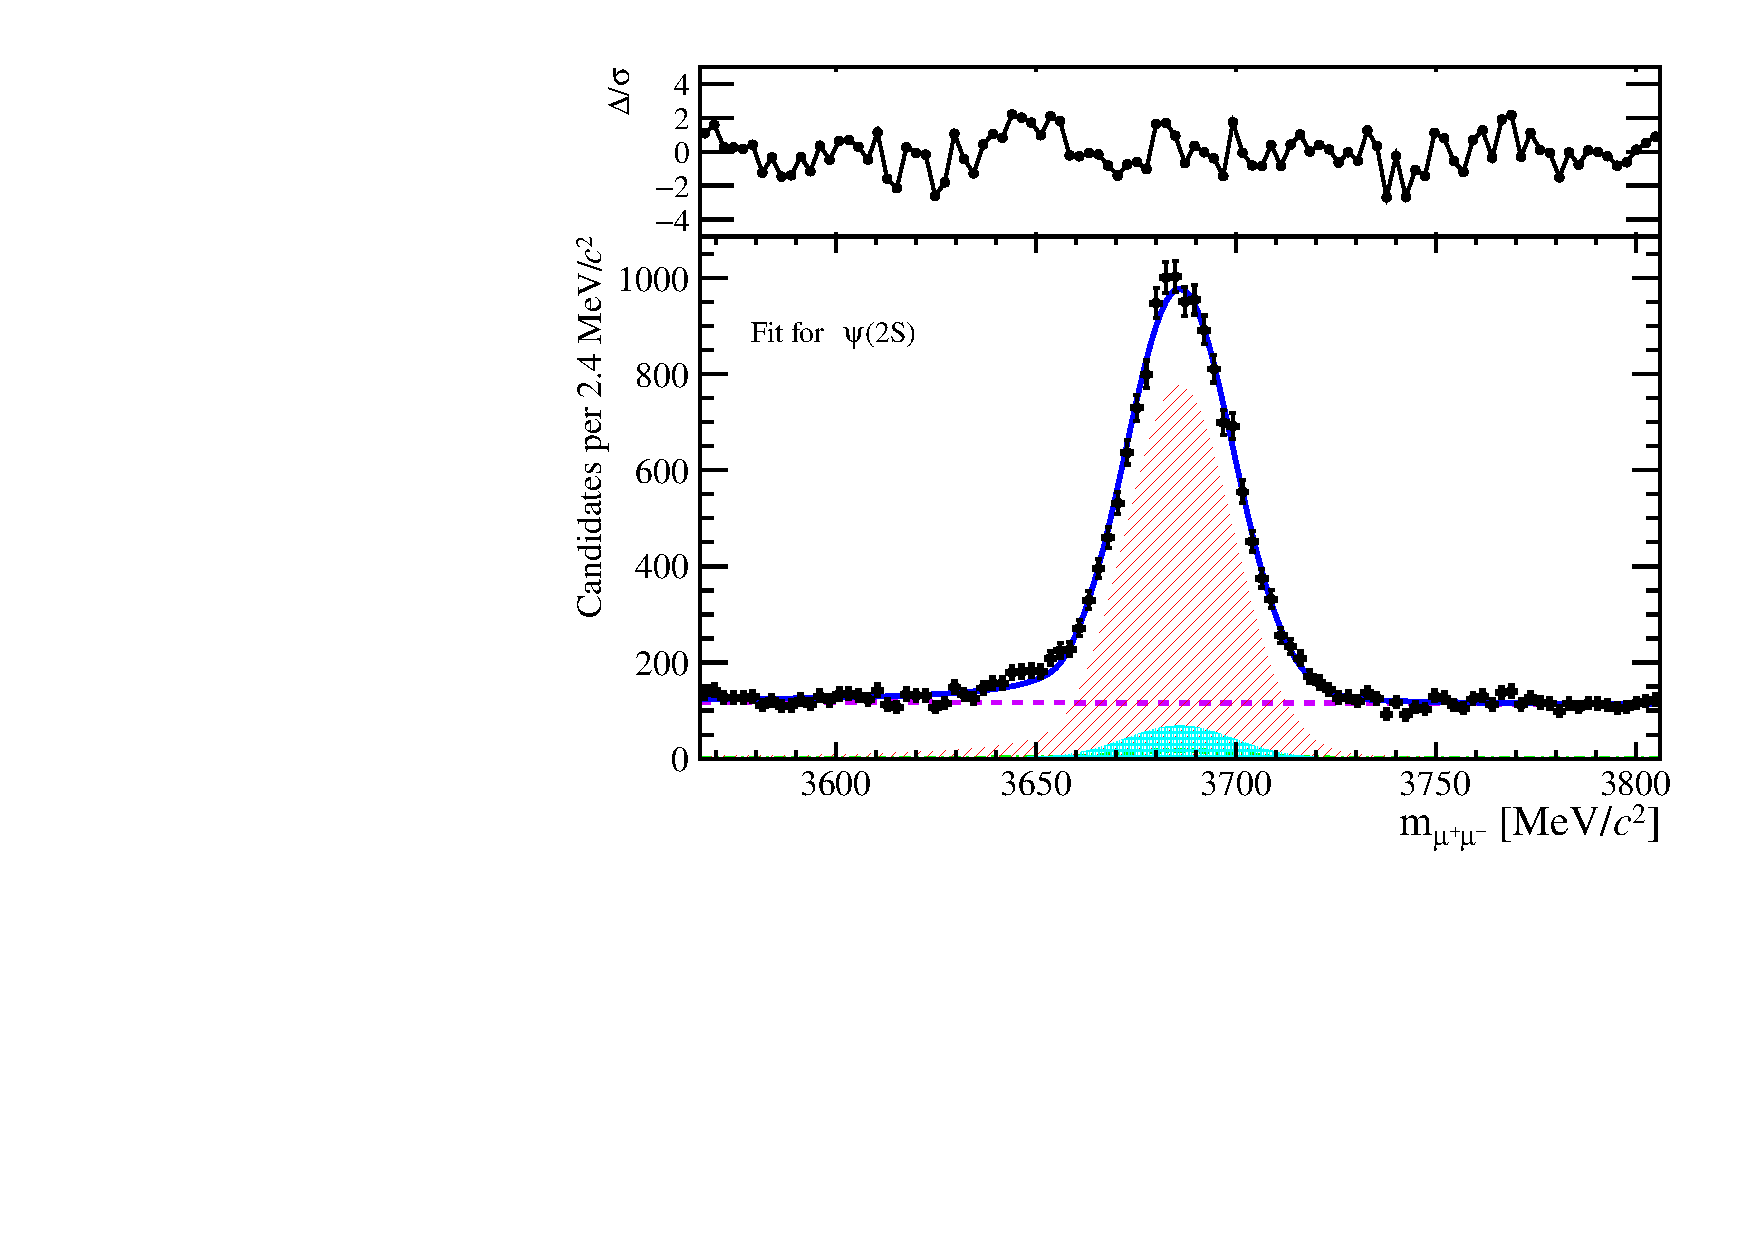
\includegraphics[width=0.47\linewidth]{pdf/Psi2S/drawmassF/n1y2pt1.pdf}
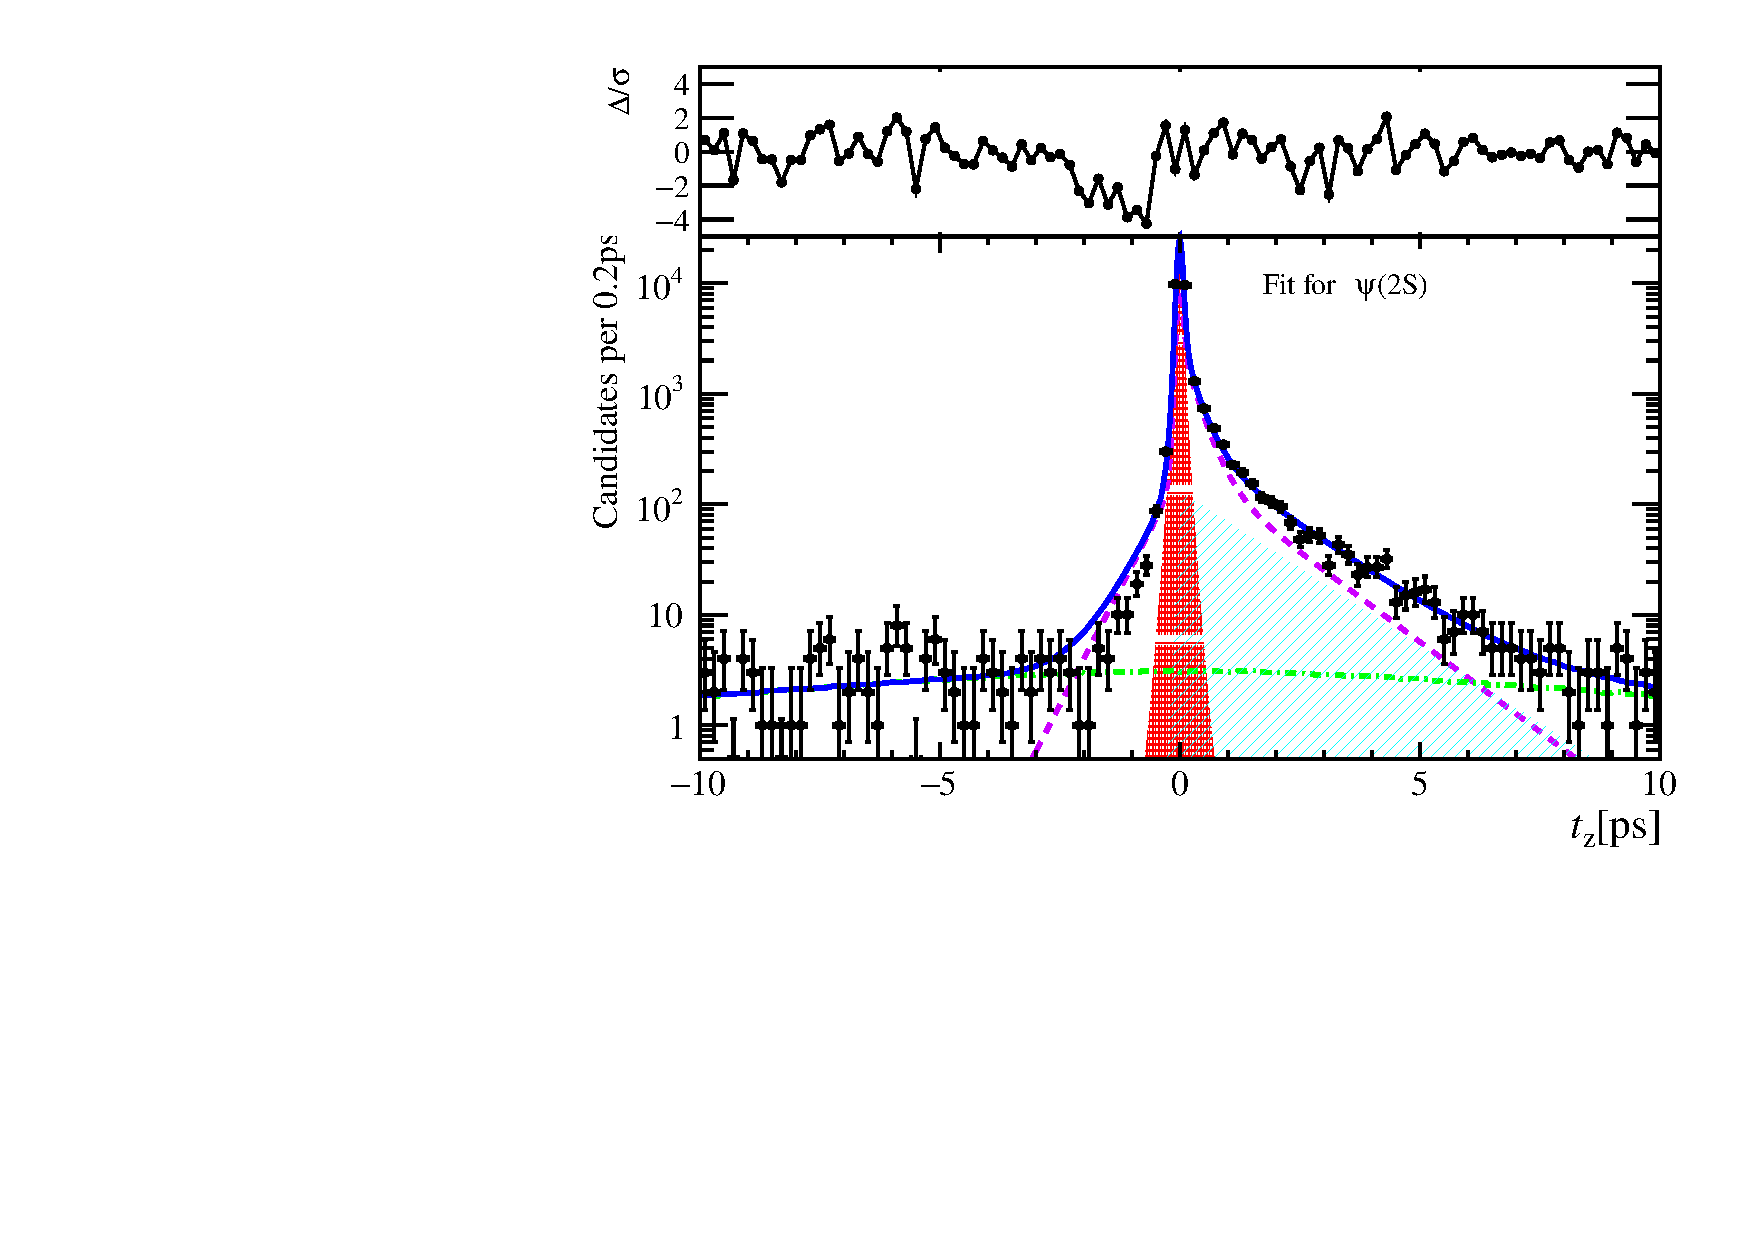
\includegraphics[width=0.47\linewidth]{pdf/Psi2S/2DFitF/n1y2pt1.pdf}
\vspace*{-0.5cm}
\end{center}
\caption{Fit results in $0\gevc<\pt<2\gevc$, $2.8<y<3.5$ and 0$\leq$nForwardTracks$<$12.}
\label{Fitn1y2pt1}
\end{figure}
\begin{figure}[H]
\begin{center}
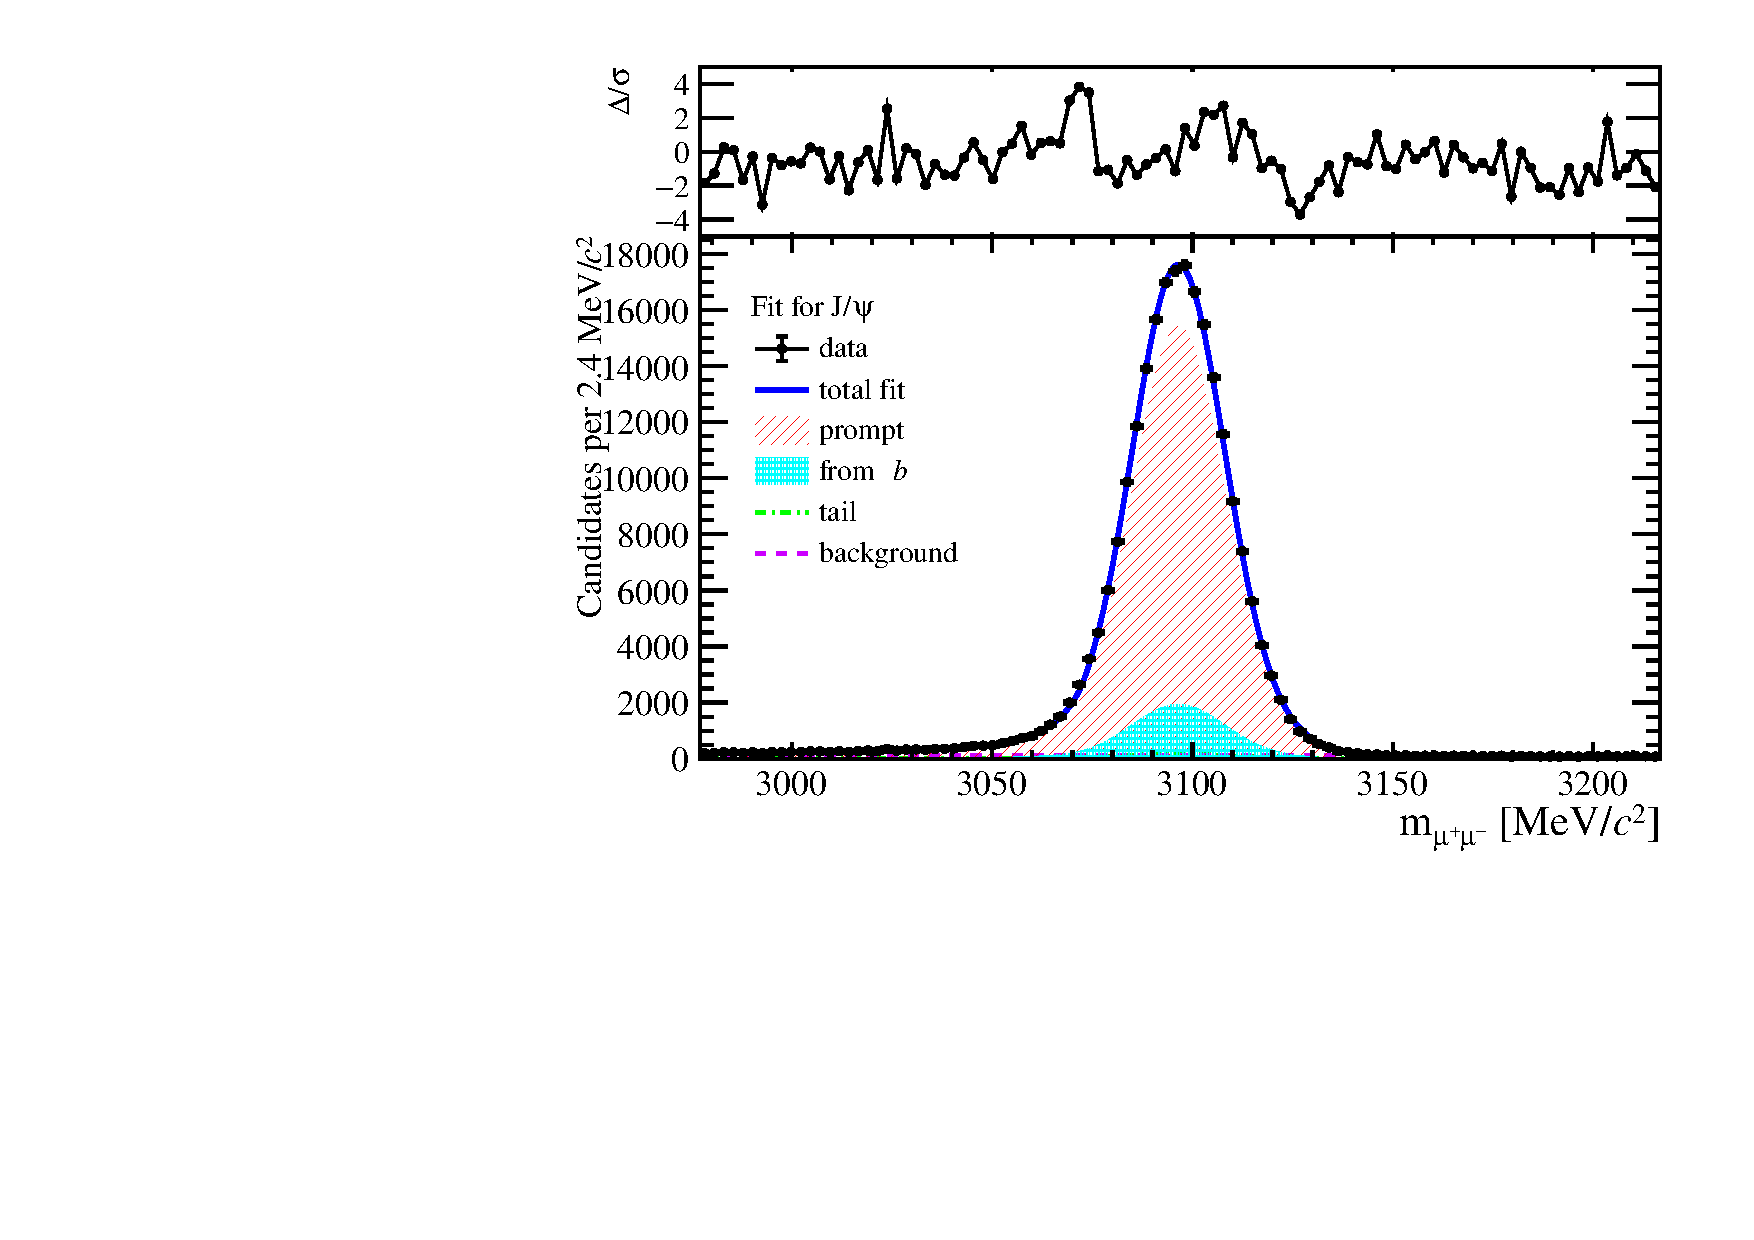
\includegraphics[width=0.47\linewidth]{pdf/Jpsi/drawmassF/n1y2pt2.pdf}
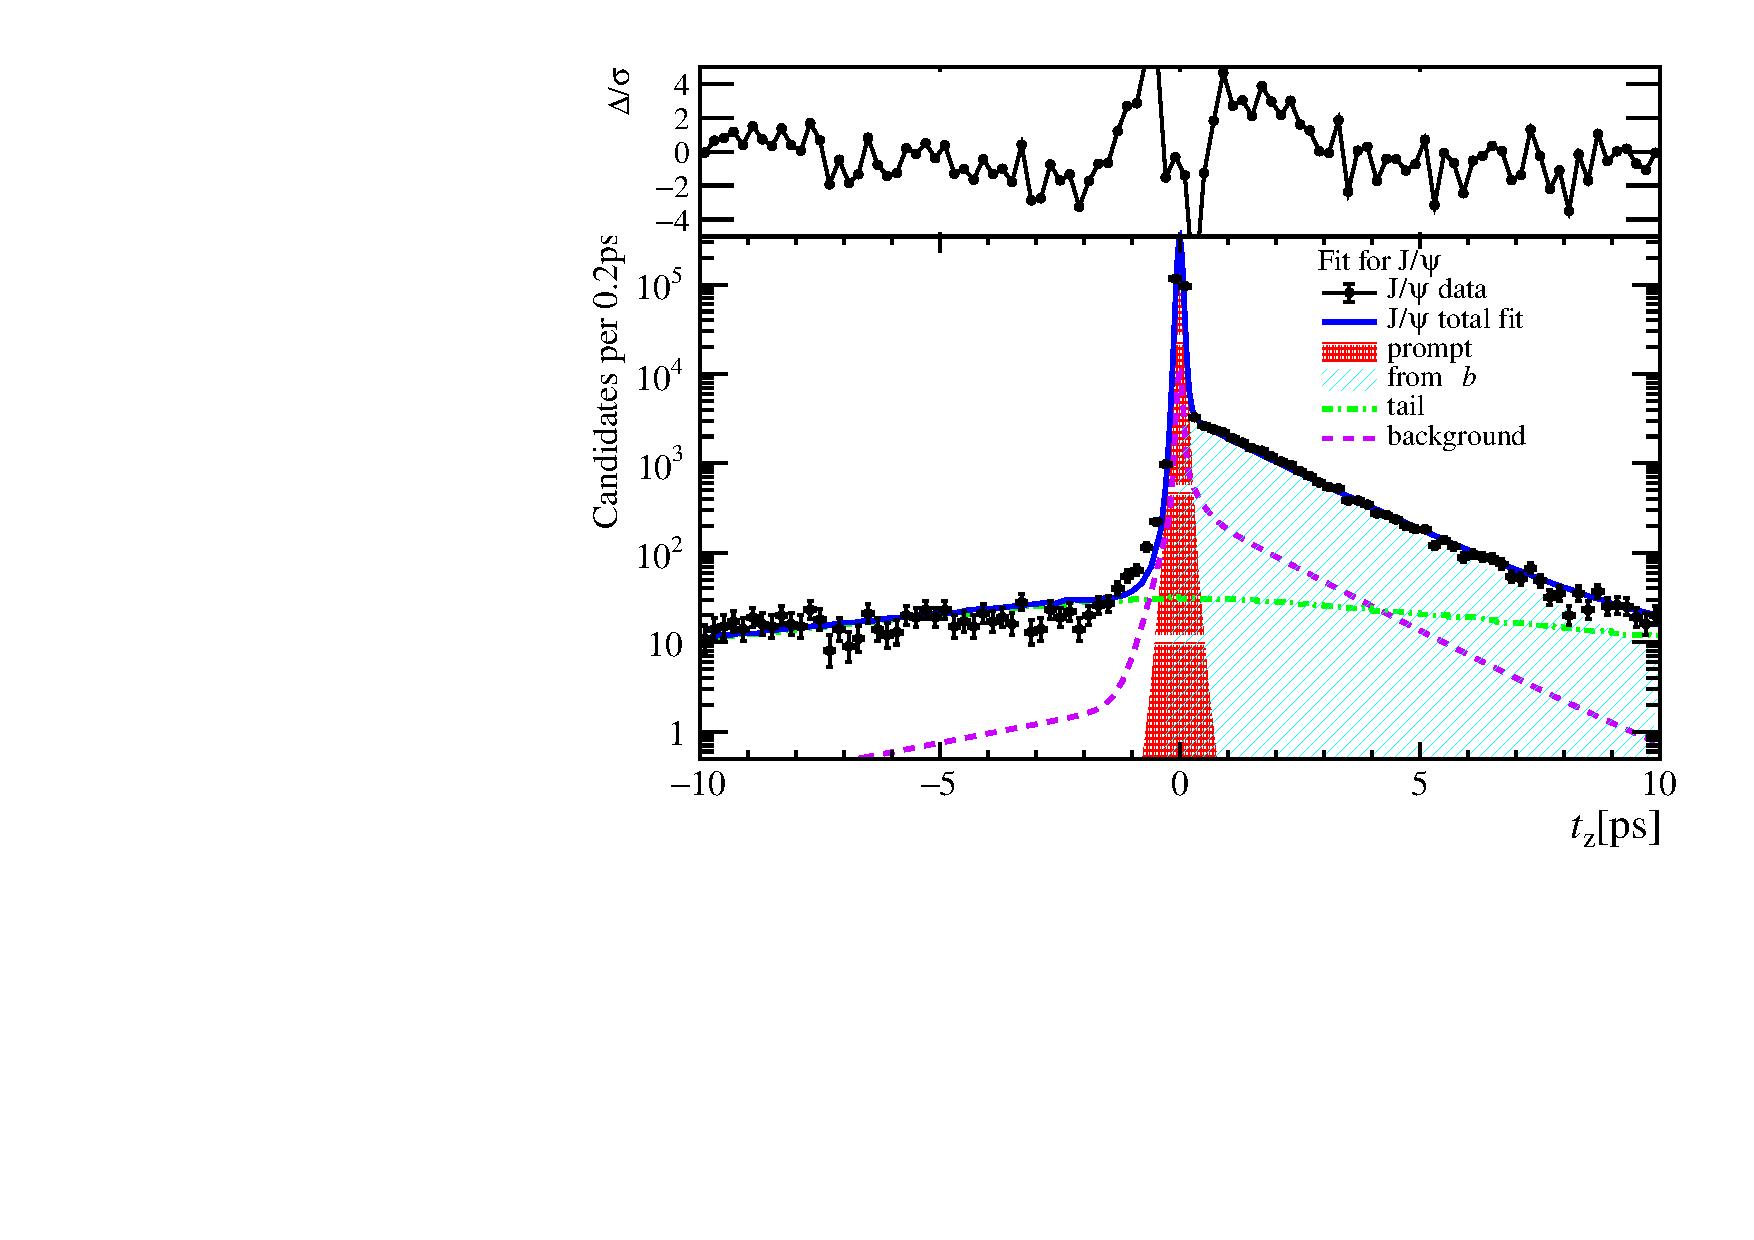
\includegraphics[width=0.47\linewidth]{pdf/Jpsi/2DFitF/n1y2pt2.pdf}
\vspace*{-0.5cm}
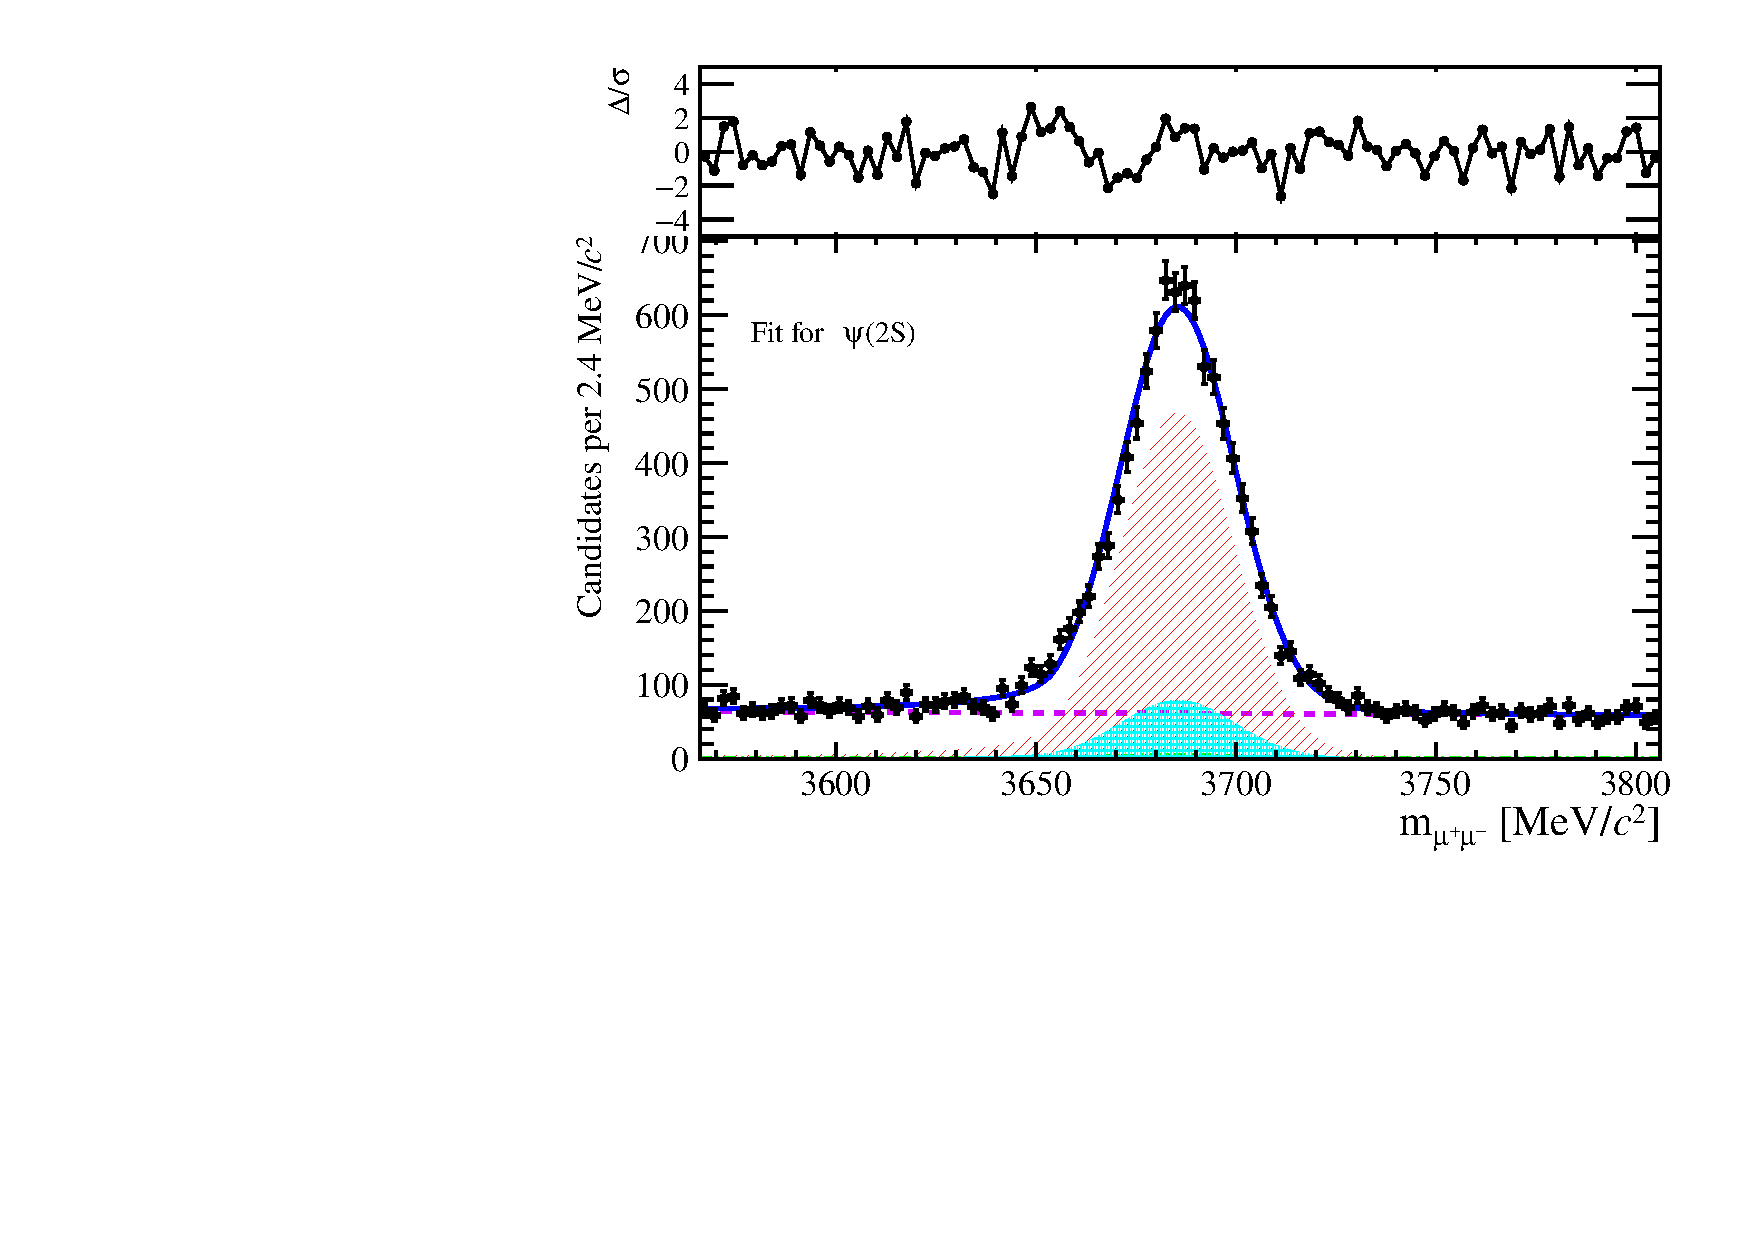
\includegraphics[width=0.47\linewidth]{pdf/Psi2S/drawmassF/n1y2pt2.pdf}
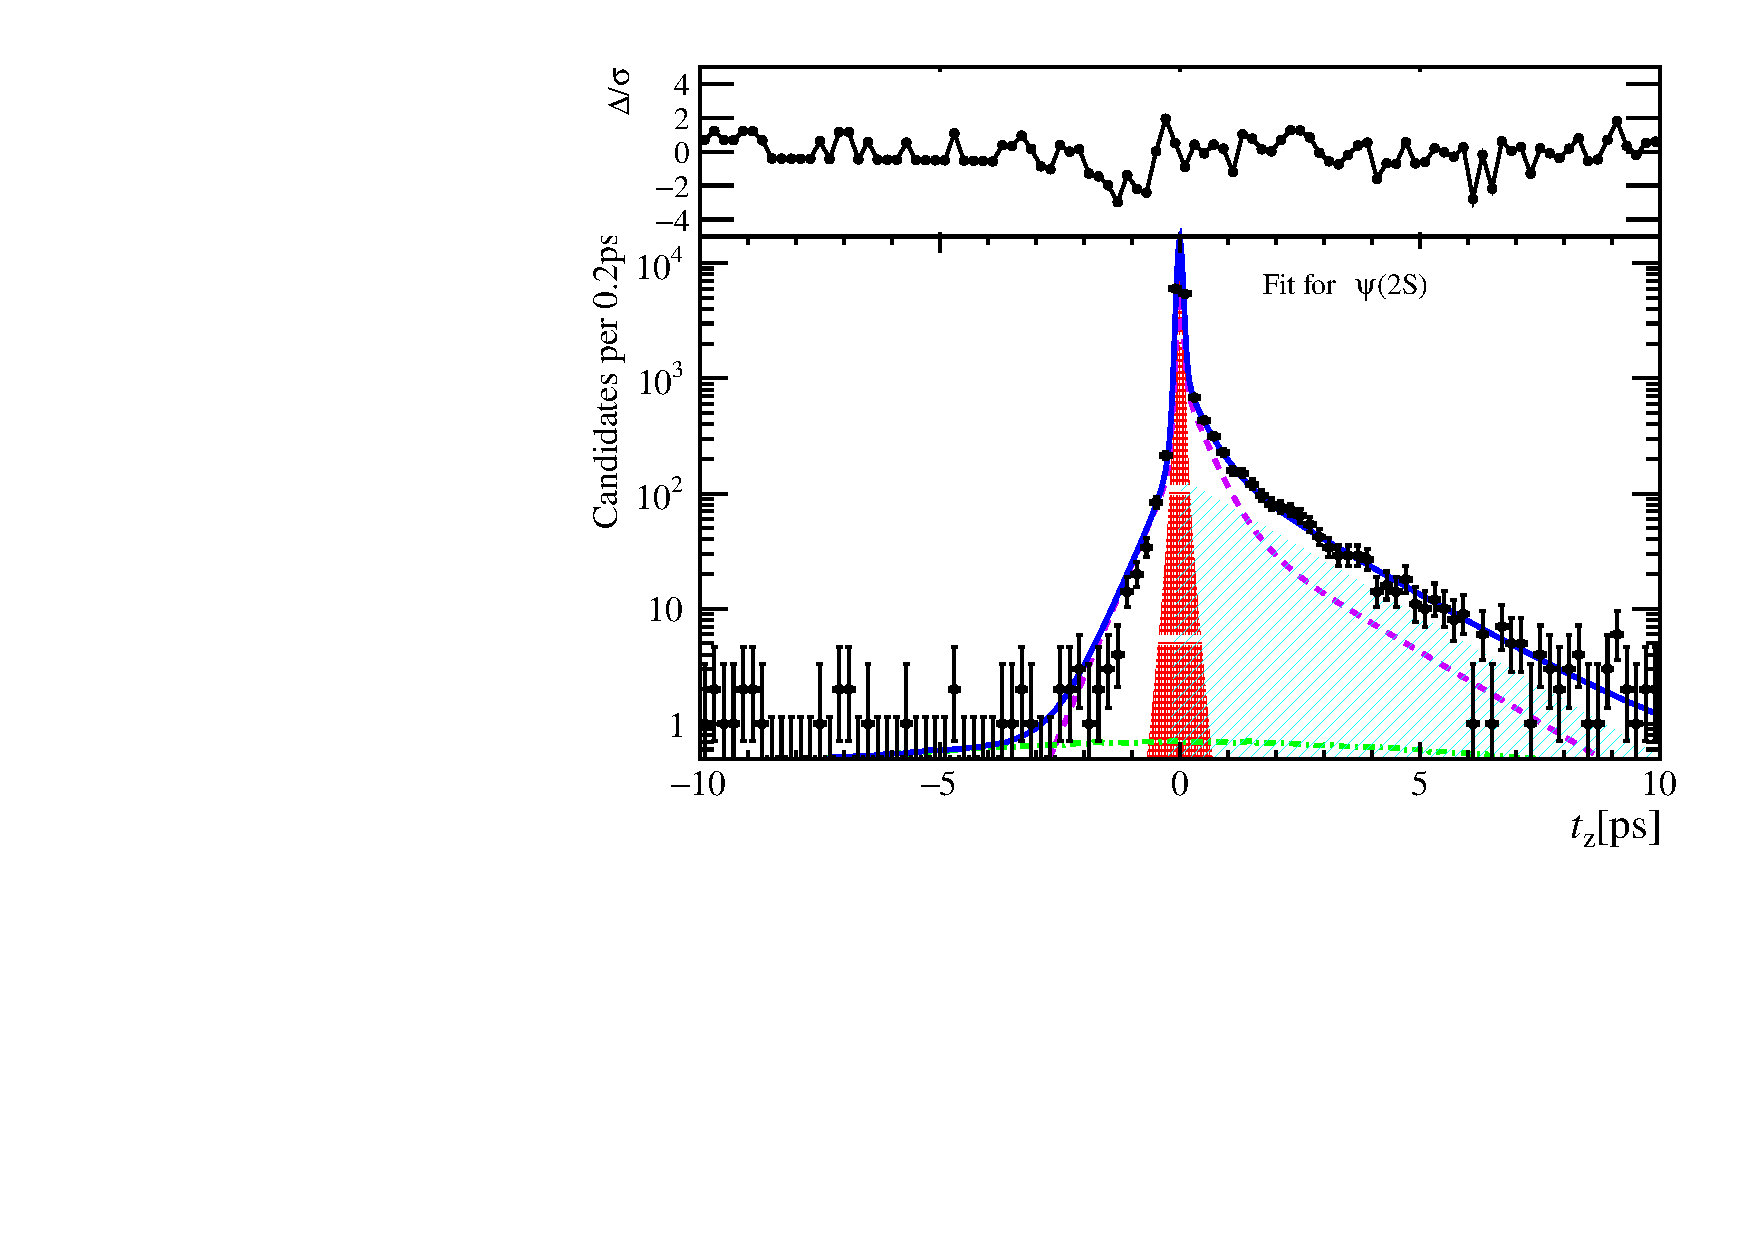
\includegraphics[width=0.47\linewidth]{pdf/Psi2S/2DFitF/n1y2pt2.pdf}
\vspace*{-0.5cm}
\end{center}
\caption{Fit results in $2\gevc<\pt<4\gevc$, $2.8<y<3.5$ and 0$\leq$nForwardTracks$<$12.}
\label{Fitn1y2pt2}
\end{figure}
\begin{figure}[H]
\begin{center}
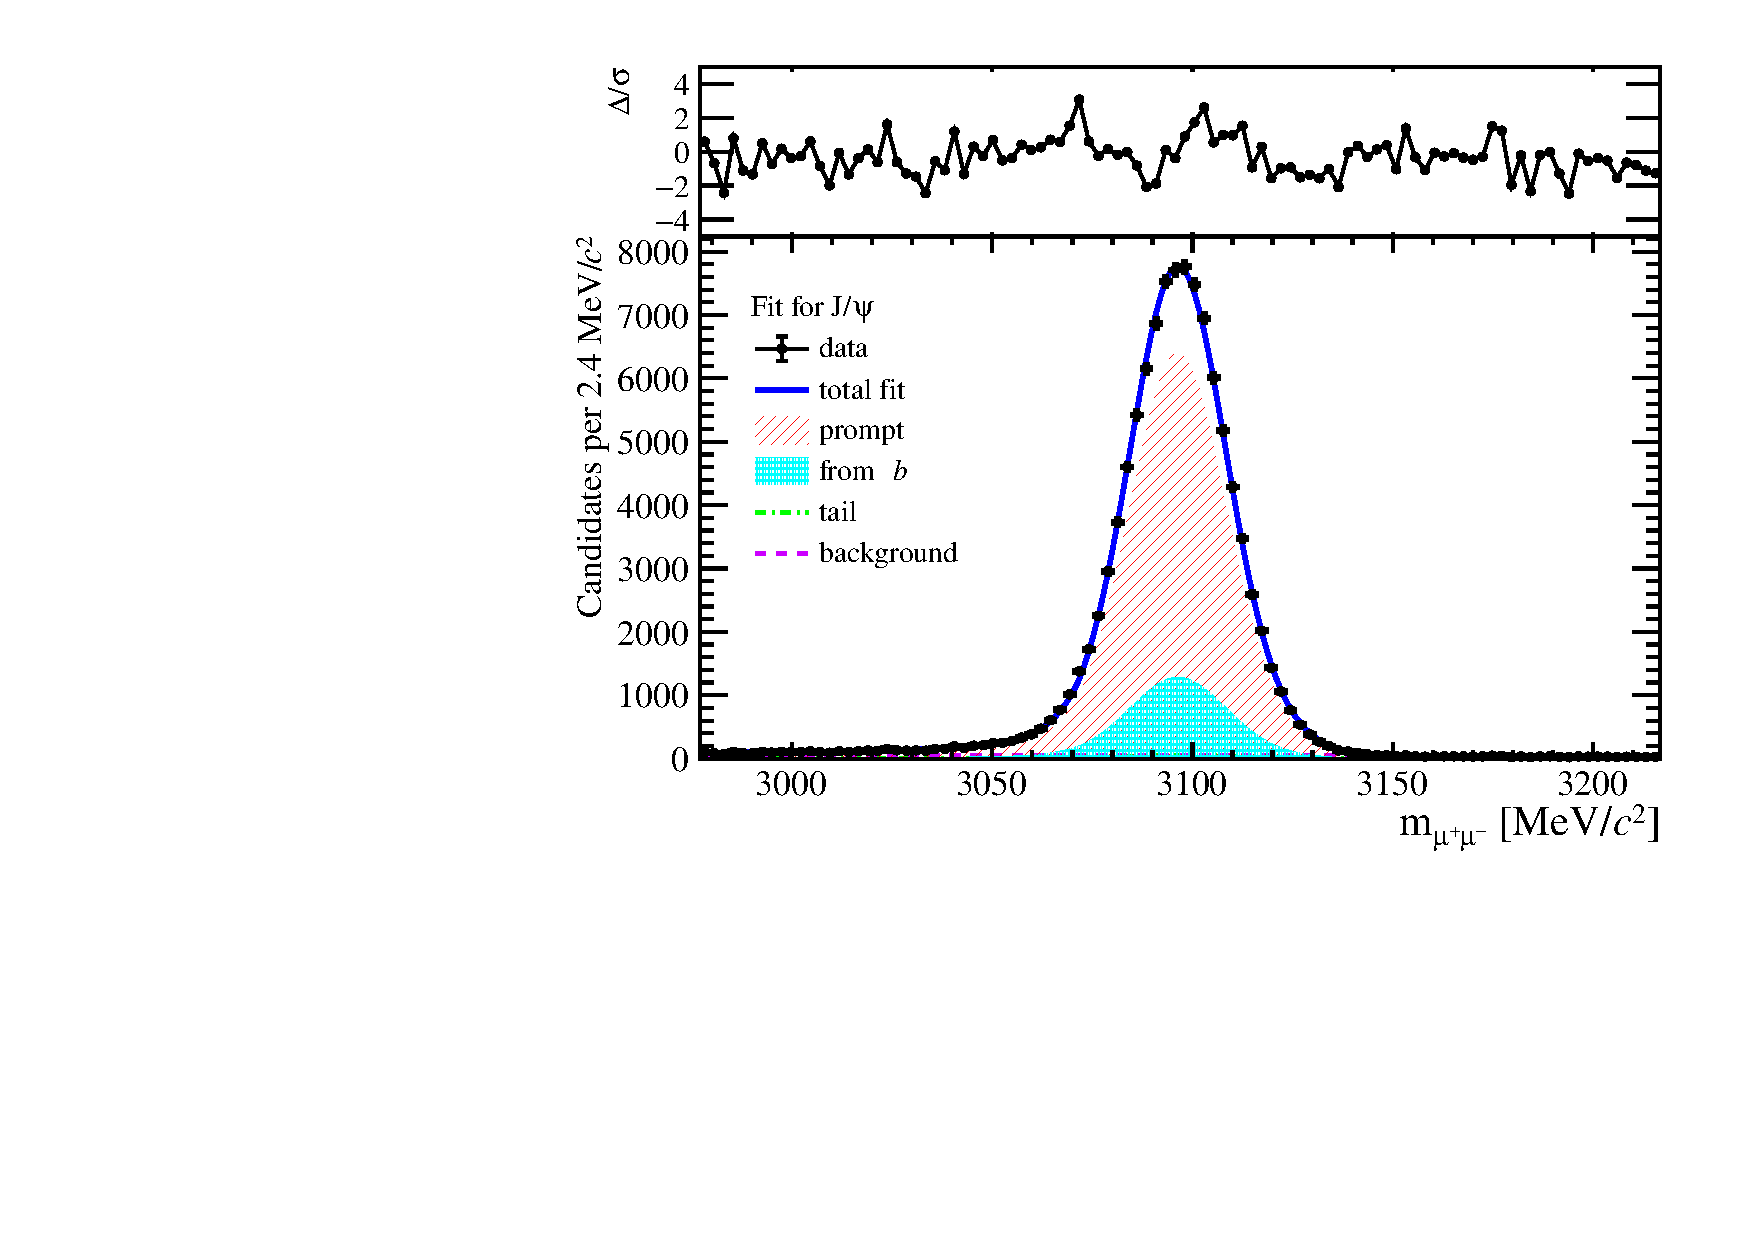
\includegraphics[width=0.47\linewidth]{pdf/Jpsi/drawmassF/n1y2pt3.pdf}
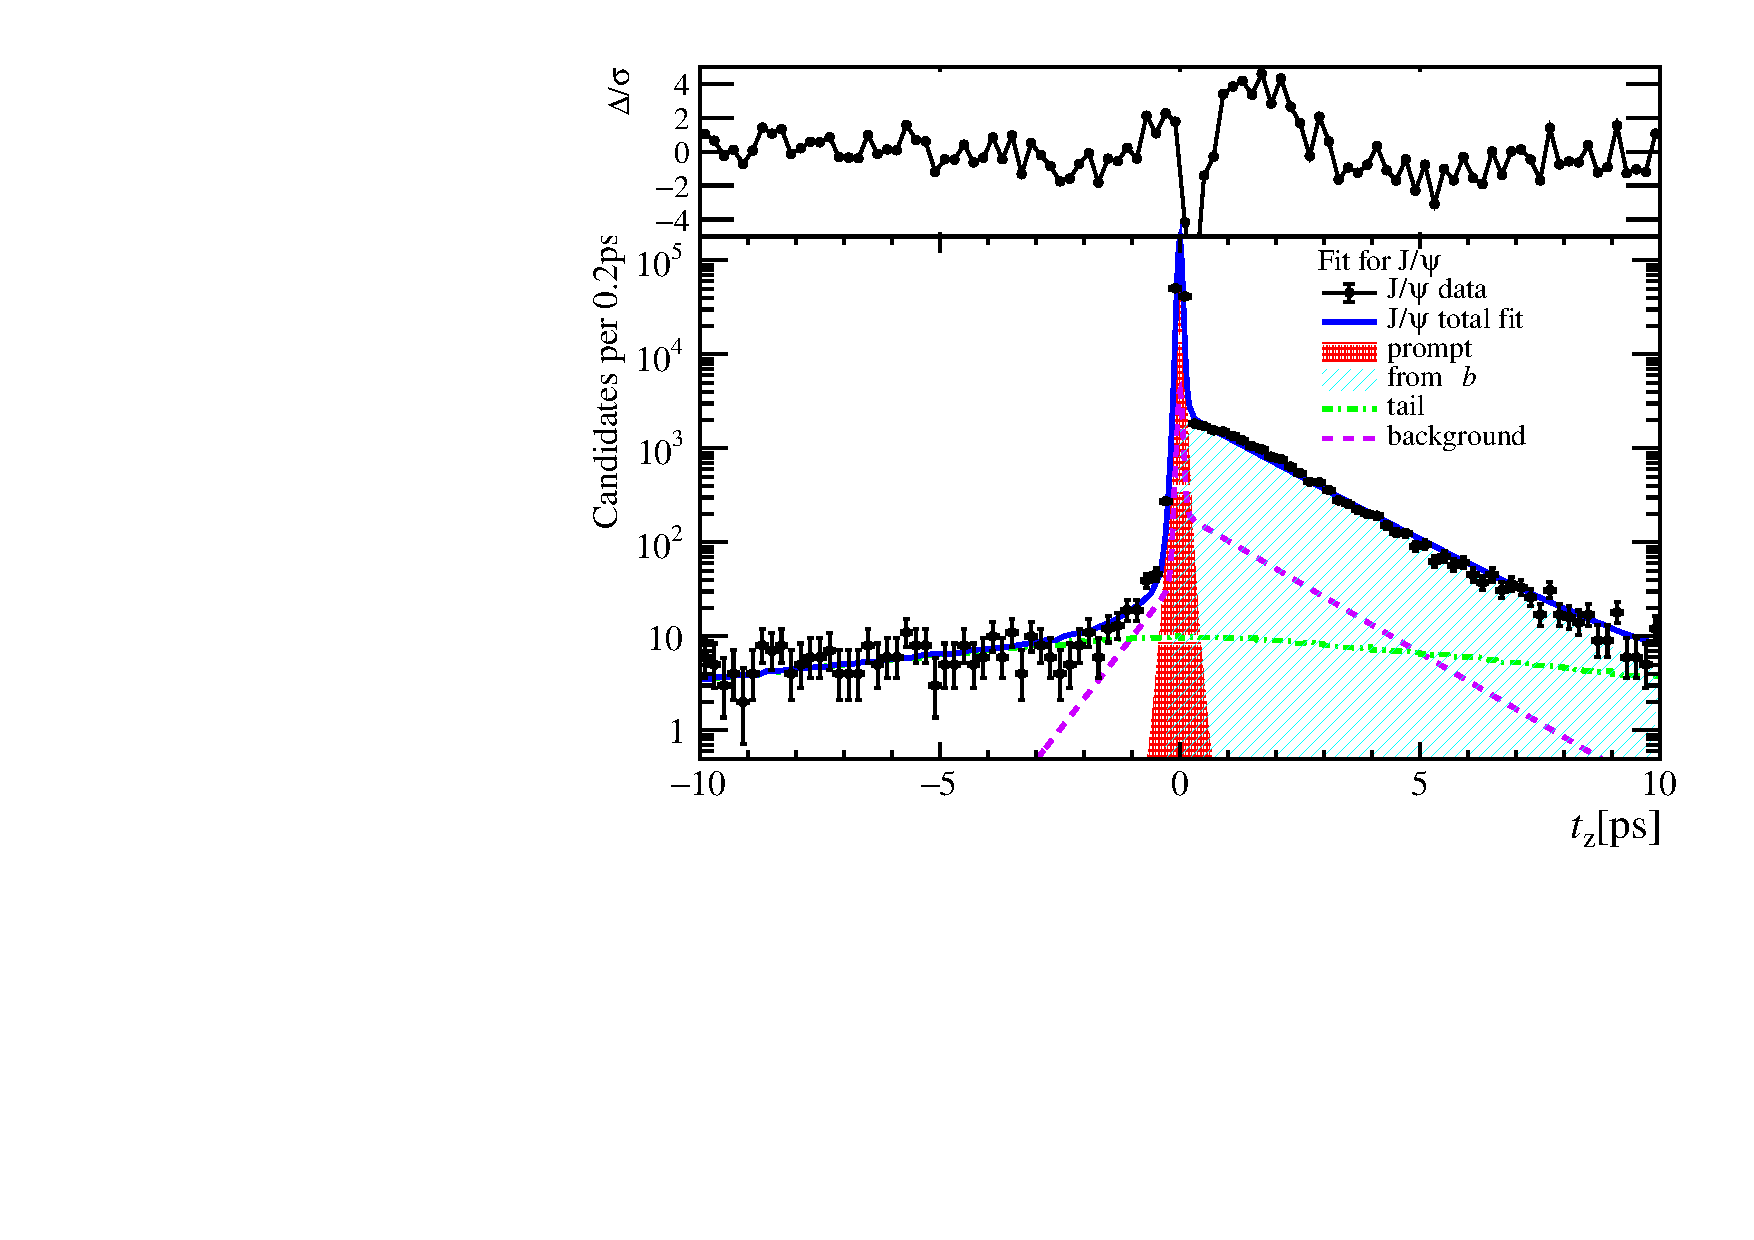
\includegraphics[width=0.47\linewidth]{pdf/Jpsi/2DFitF/n1y2pt3.pdf}
\vspace*{-0.5cm}
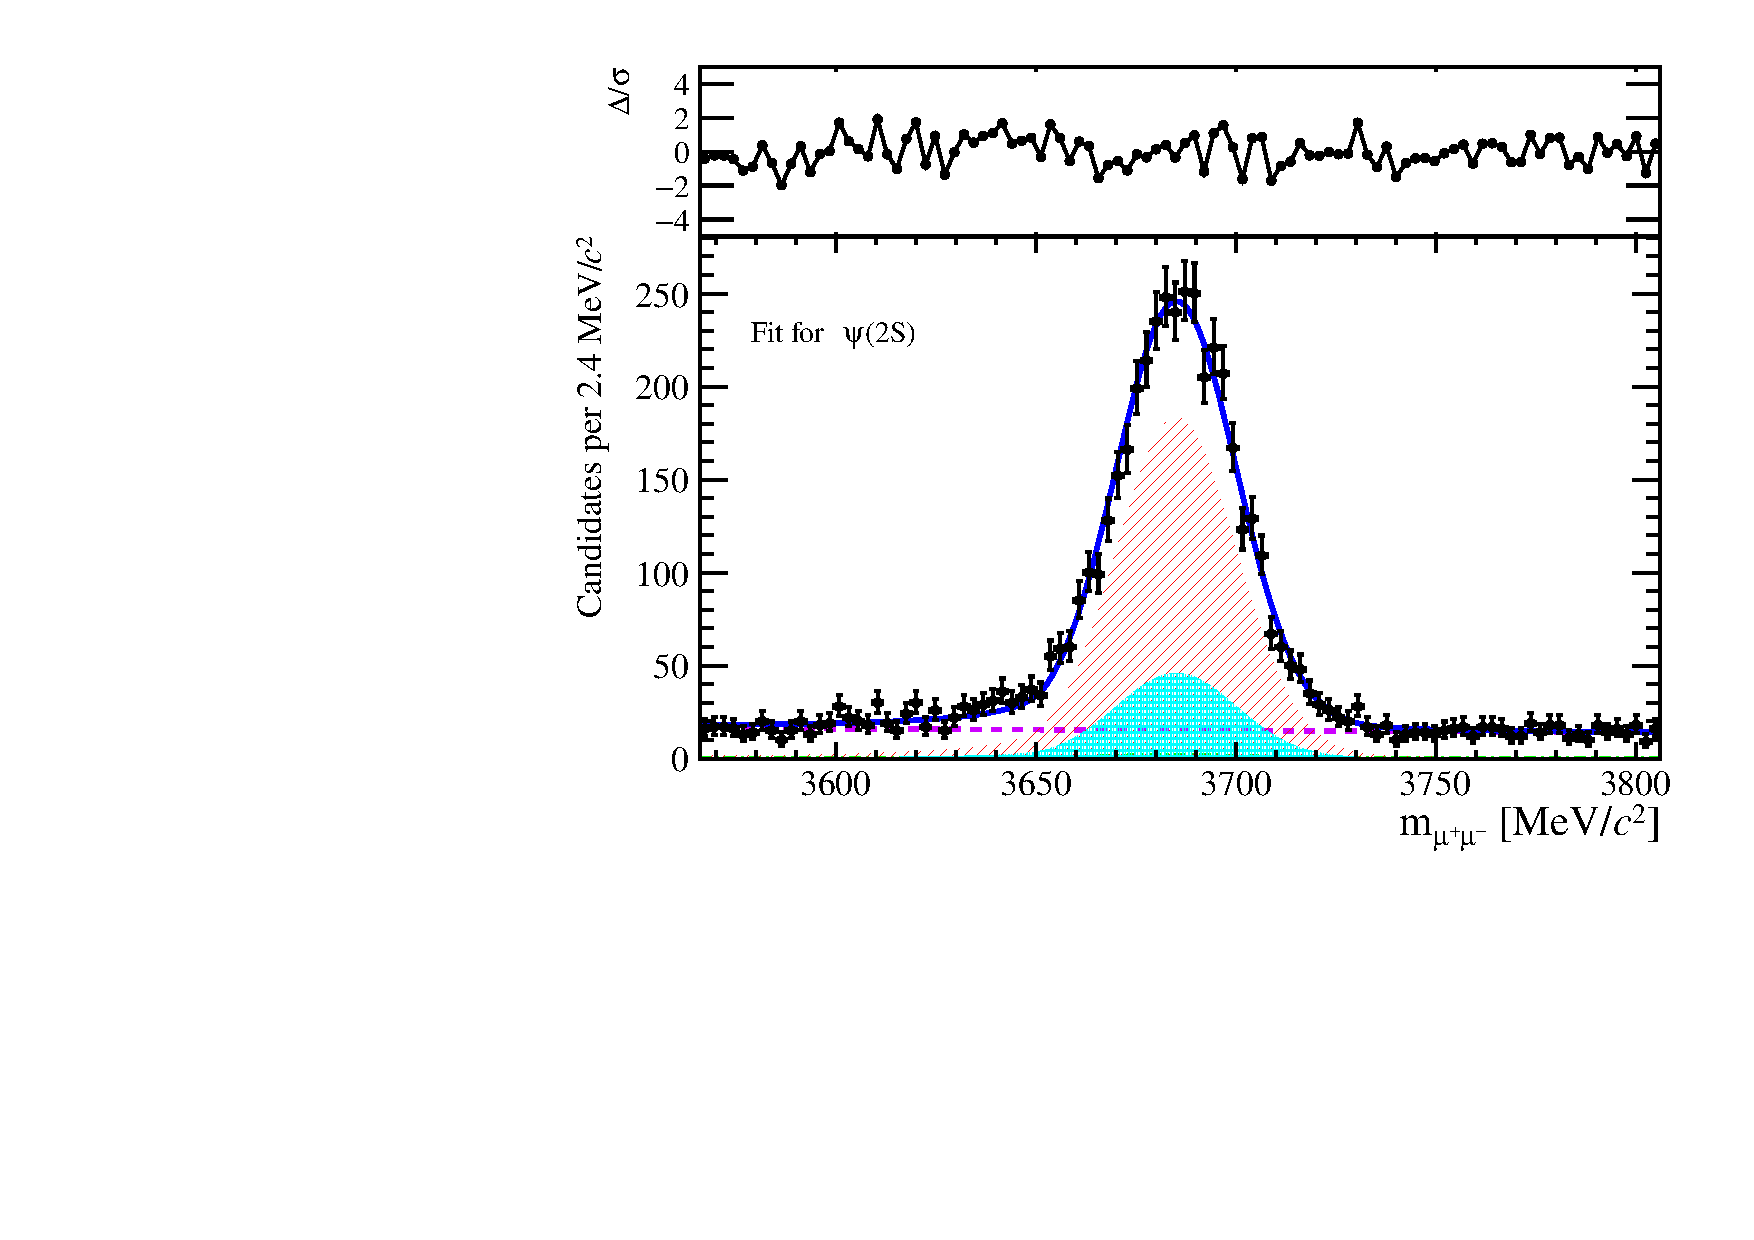
\includegraphics[width=0.47\linewidth]{pdf/Psi2S/drawmassF/n1y2pt3.pdf}
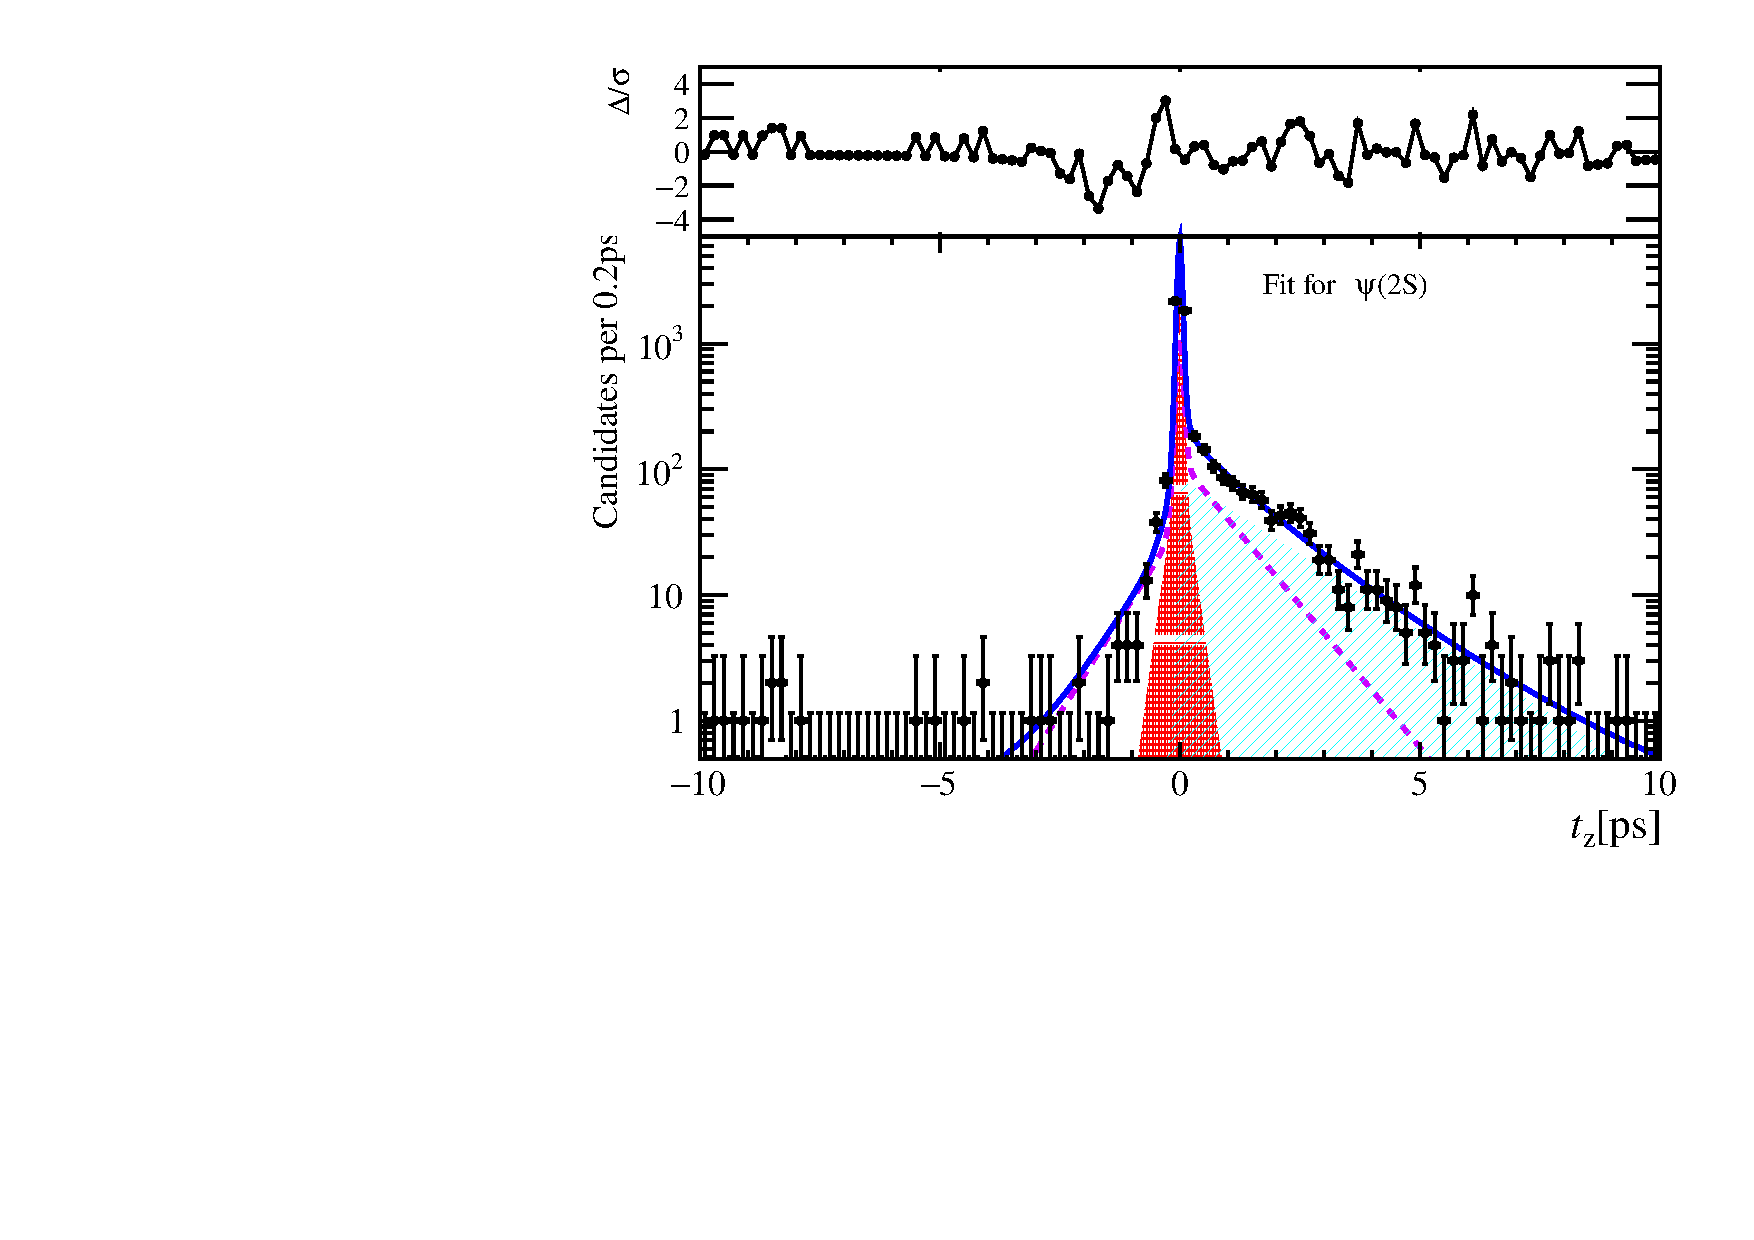
\includegraphics[width=0.47\linewidth]{pdf/Psi2S/2DFitF/n1y2pt3.pdf}
\vspace*{-0.5cm}
\end{center}
\caption{Fit results in $4\gevc<\pt<6\gevc$, $2.8<y<3.5$ and 0$\leq$nForwardTracks$<$12.}
\label{Fitn1y2pt3}
\end{figure}
\begin{figure}[H]
\begin{center}
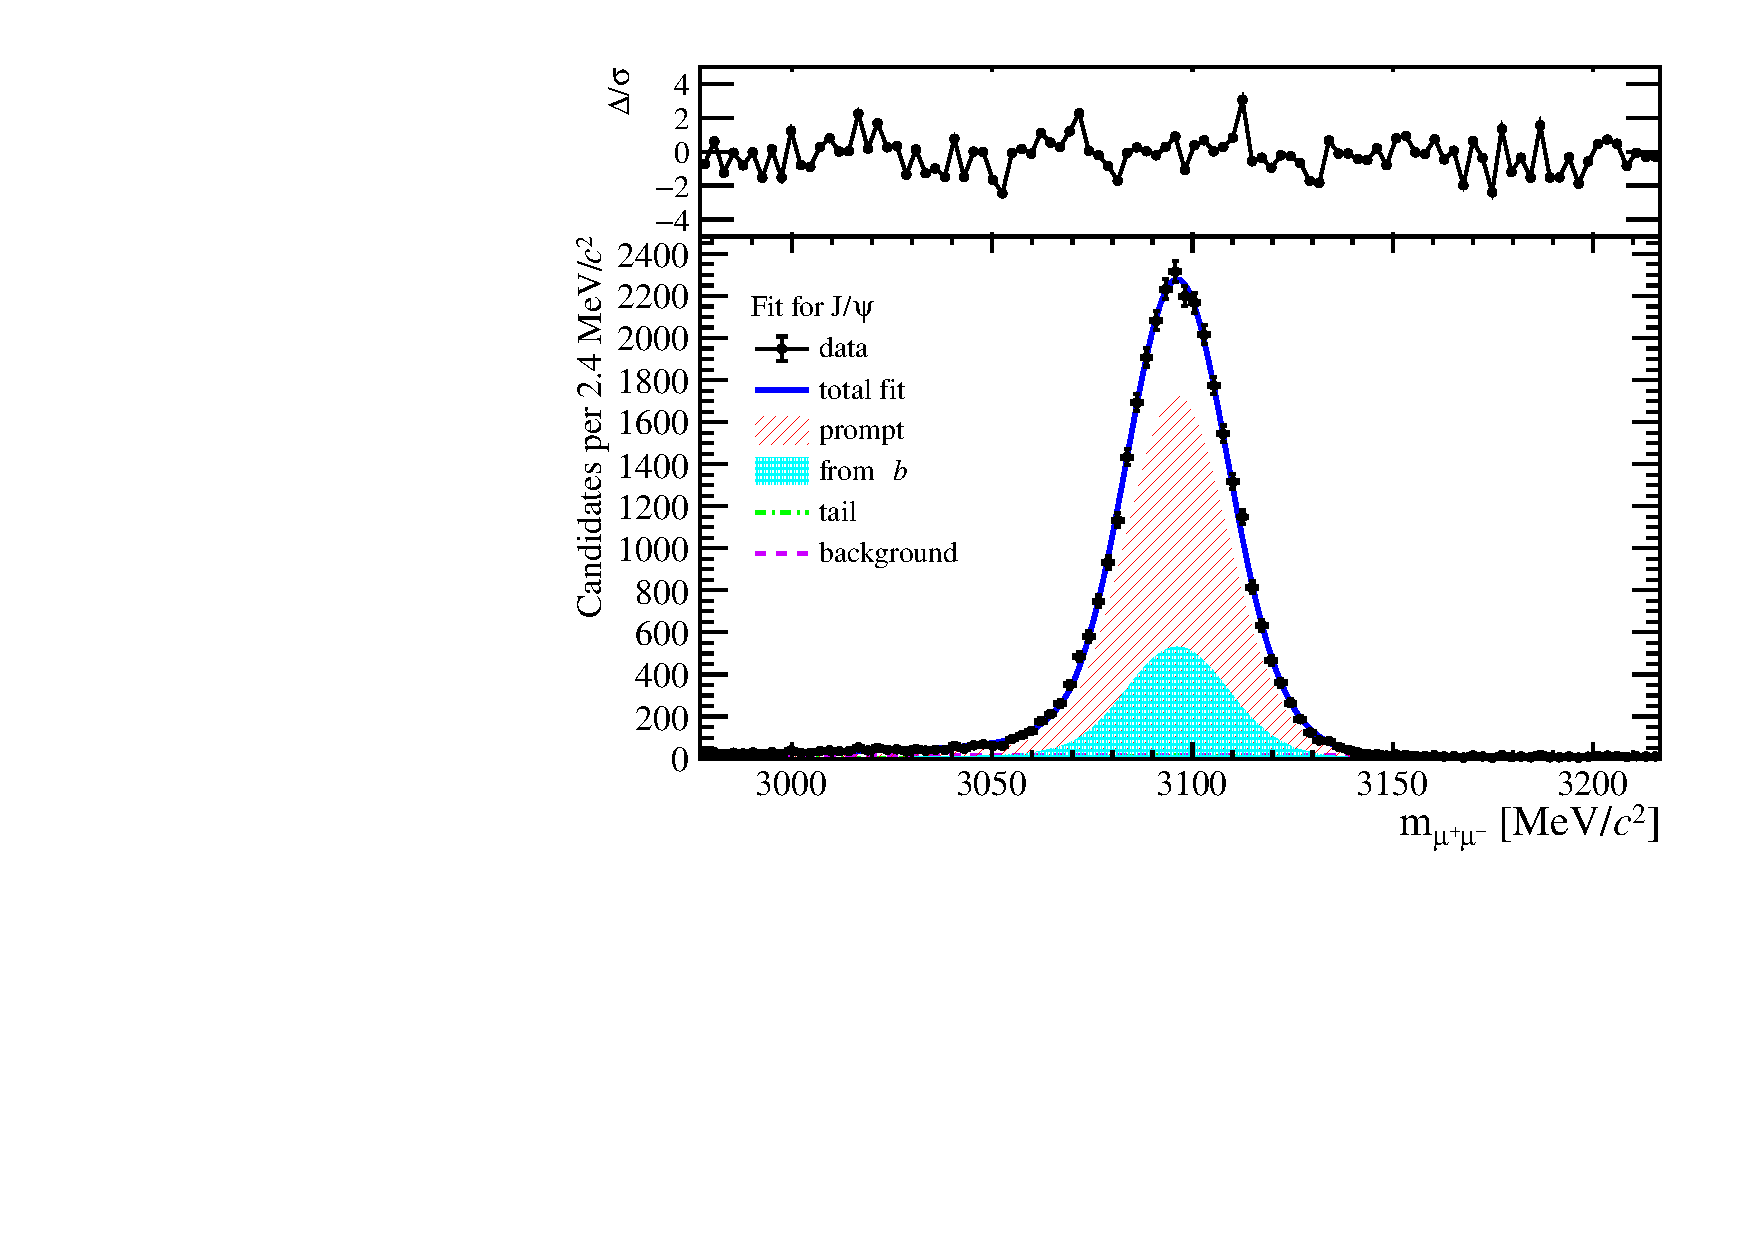
\includegraphics[width=0.47\linewidth]{pdf/Jpsi/drawmassF/n1y2pt4.pdf}
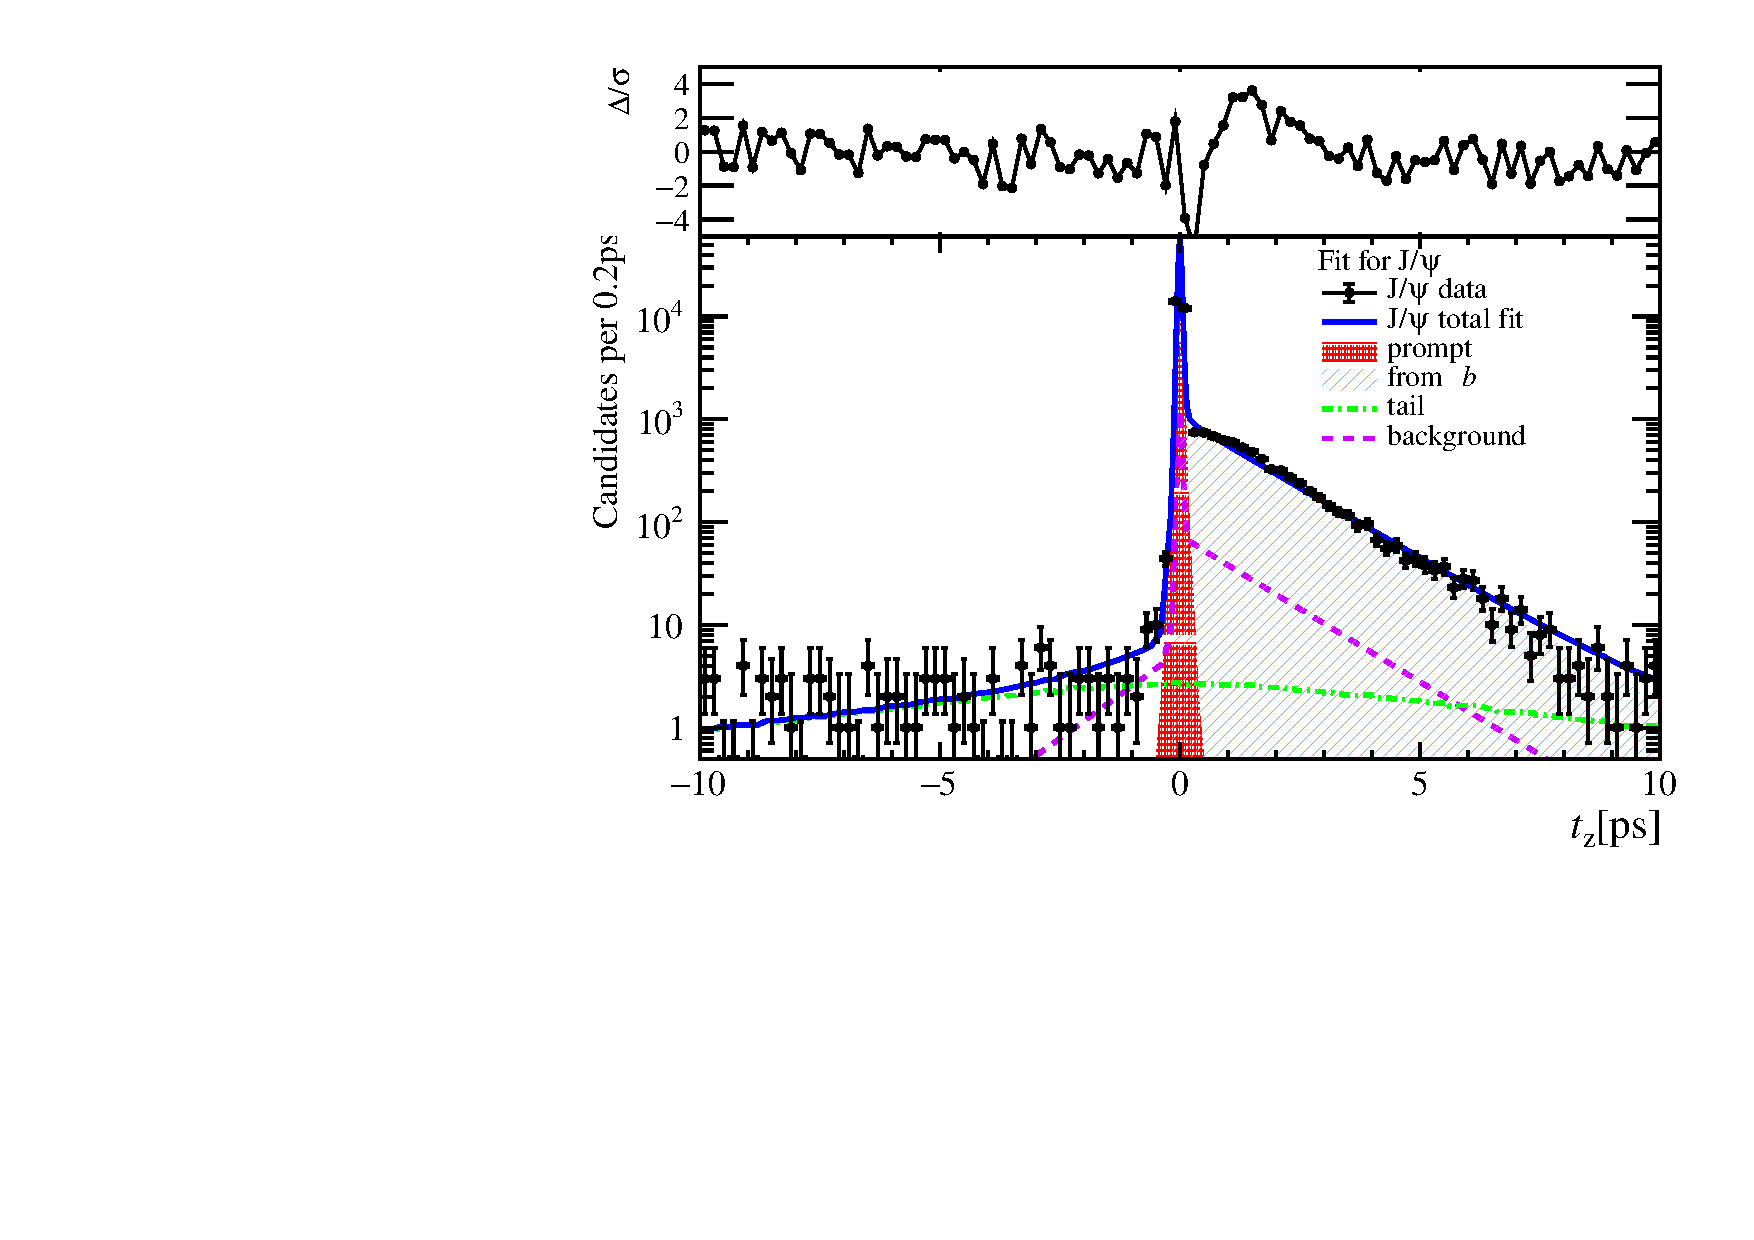
\includegraphics[width=0.47\linewidth]{pdf/Jpsi/2DFitF/n1y2pt4.pdf}
\vspace*{-0.5cm}
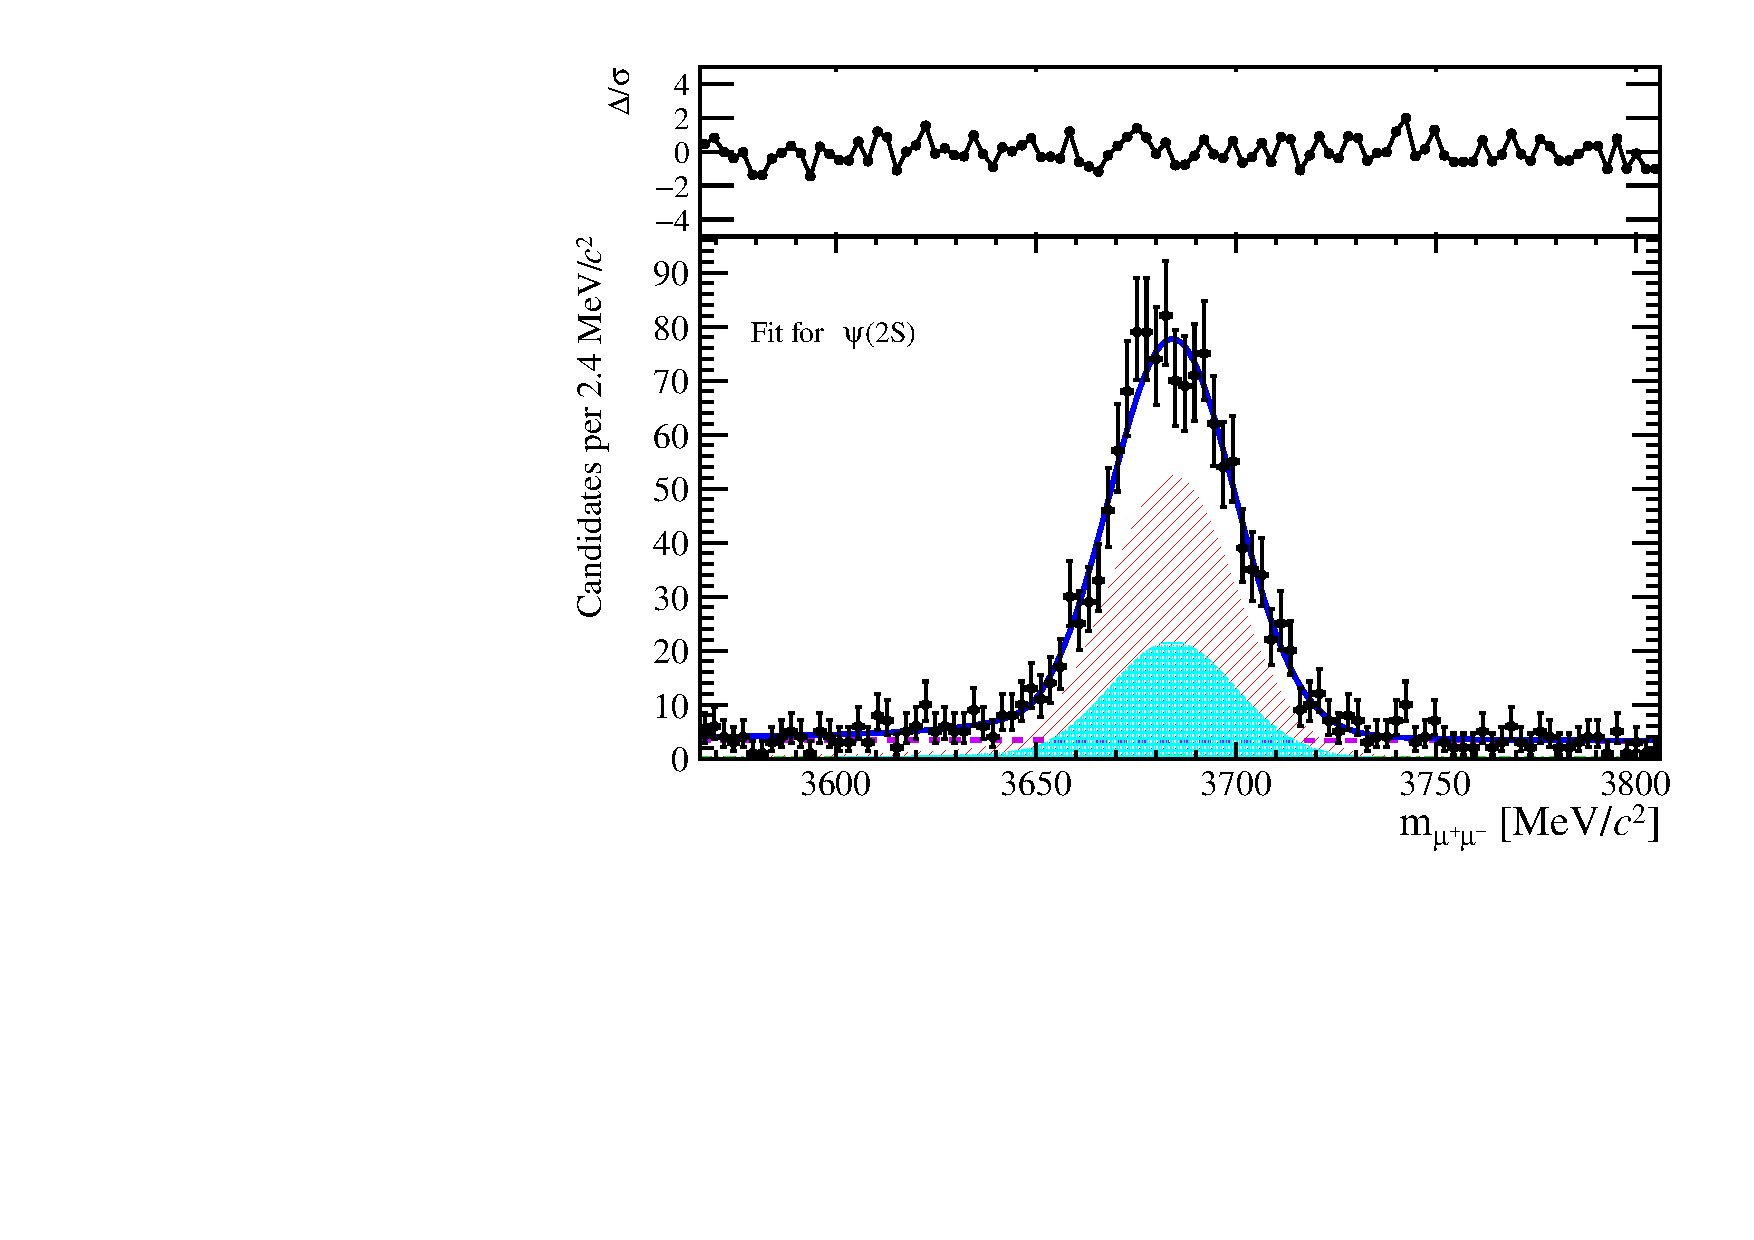
\includegraphics[width=0.47\linewidth]{pdf/Psi2S/drawmassF/n1y2pt4.pdf}
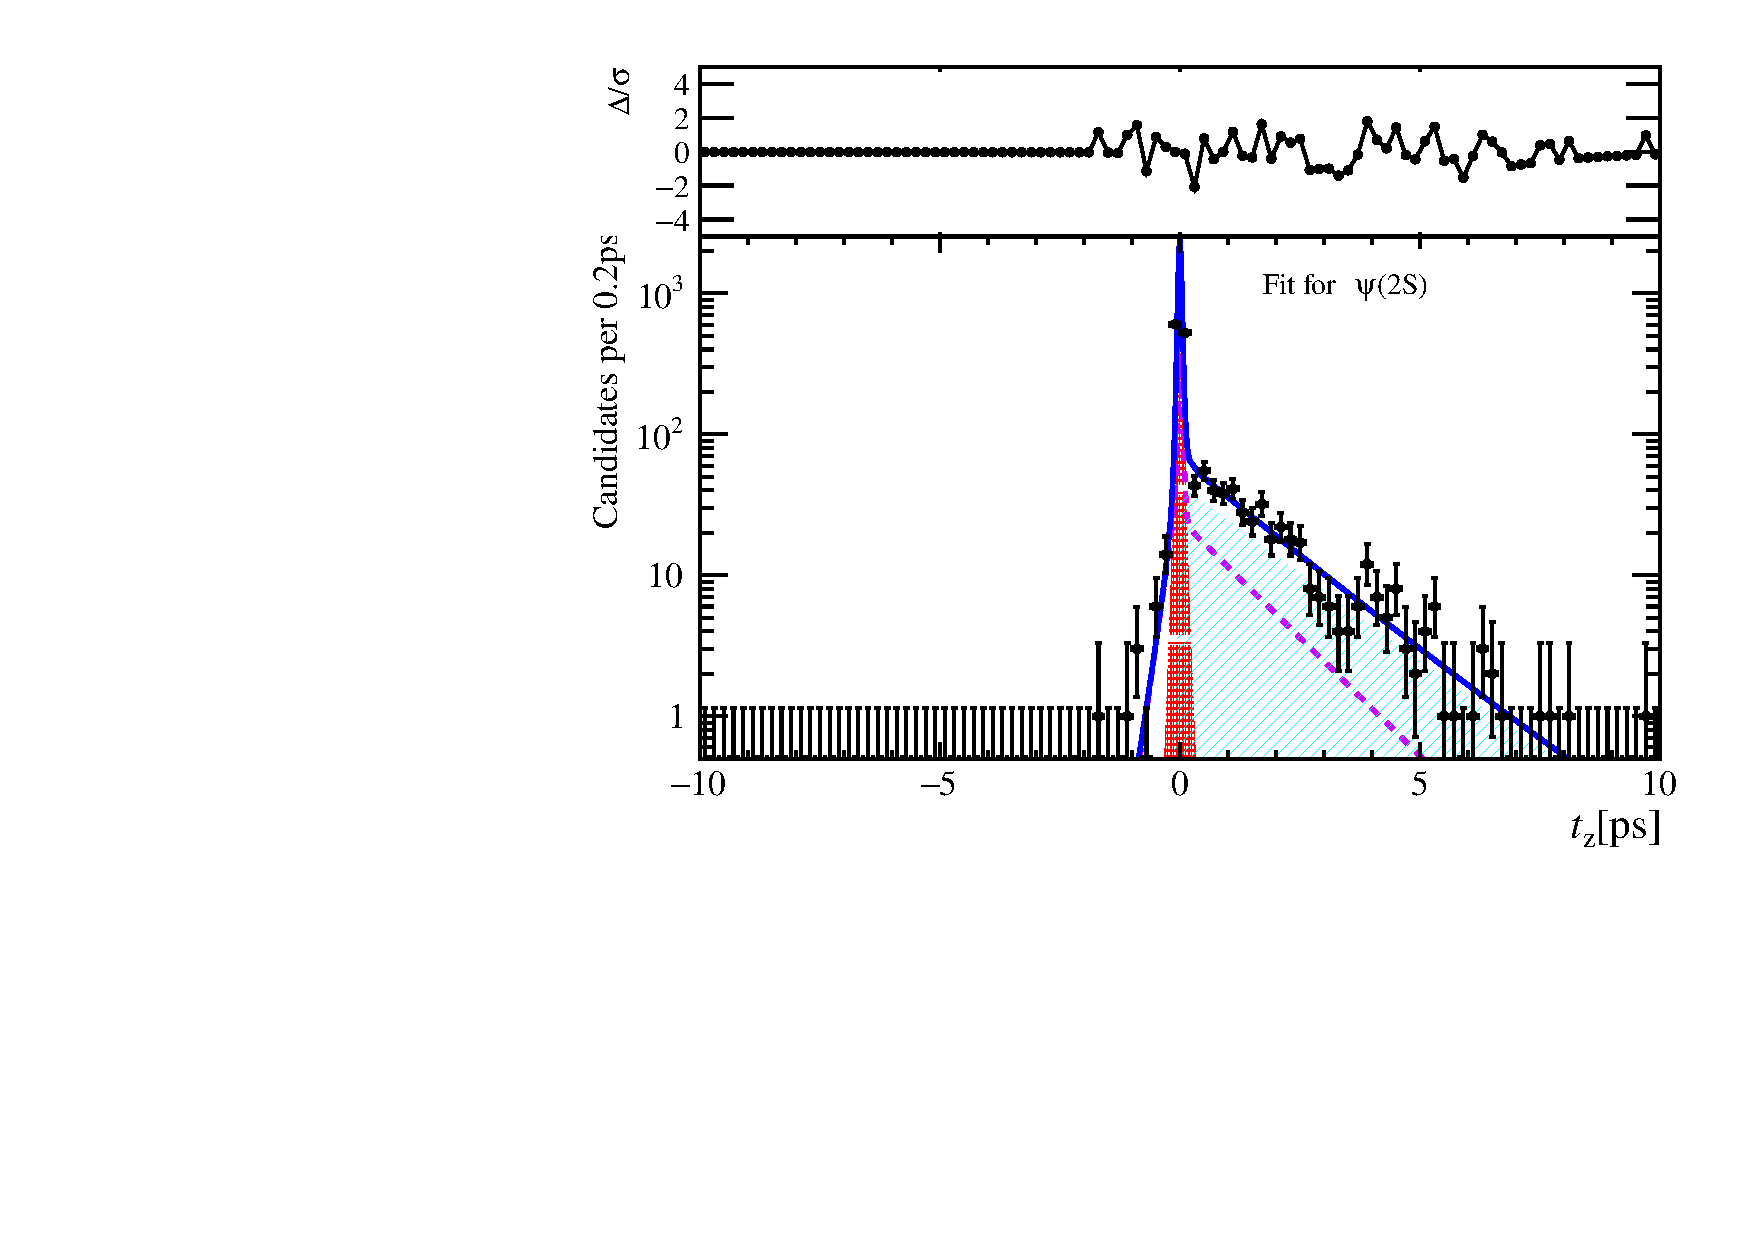
\includegraphics[width=0.47\linewidth]{pdf/Psi2S/2DFitF/n1y2pt4.pdf}
\vspace*{-0.5cm}
\end{center}
\caption{Fit results in $6\gevc<\pt<8\gevc$, $2.8<y<3.5$ and 0$\leq$nForwardTracks$<$12.}
\label{Fitn1y2pt4}
\end{figure}
\begin{figure}[H]
\begin{center}
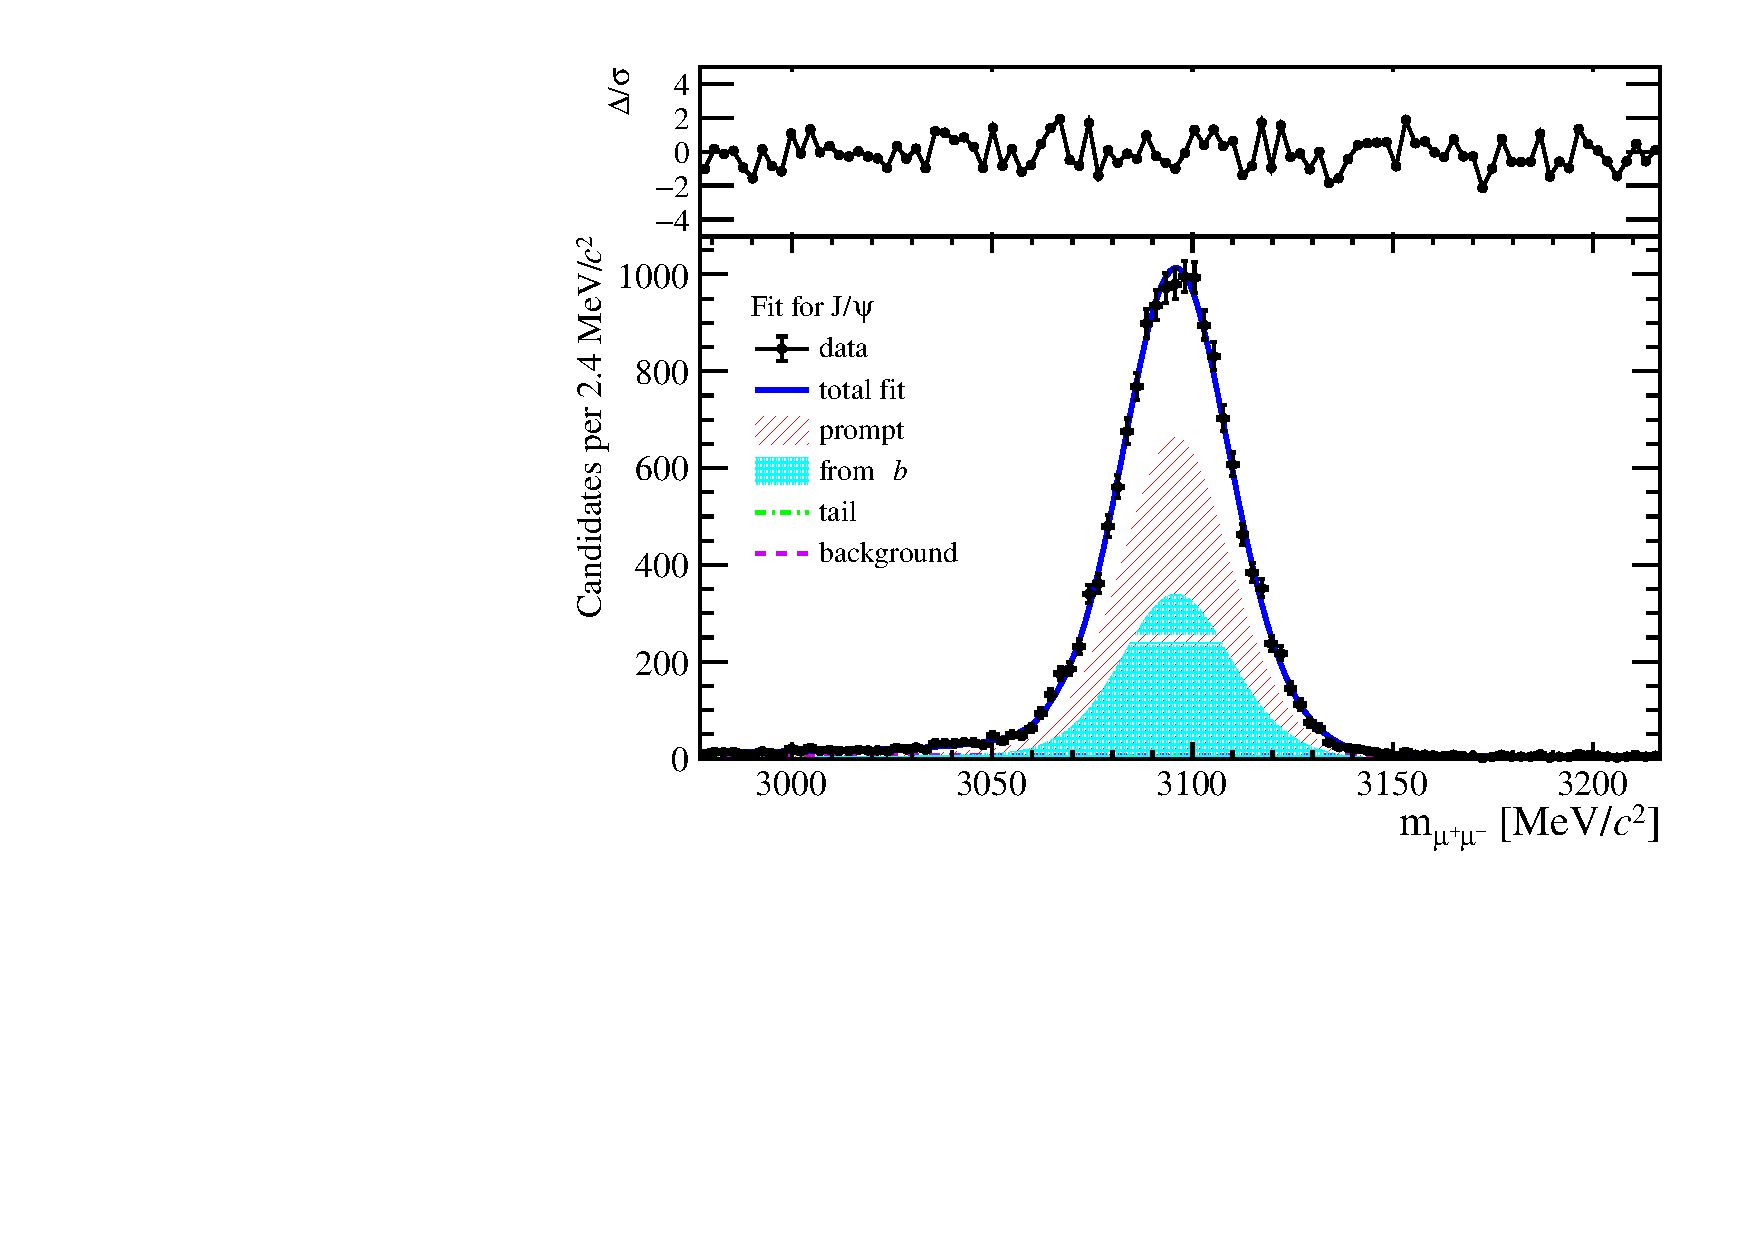
\includegraphics[width=0.47\linewidth]{pdf/Jpsi/drawmassF/n1y2pt5.pdf}
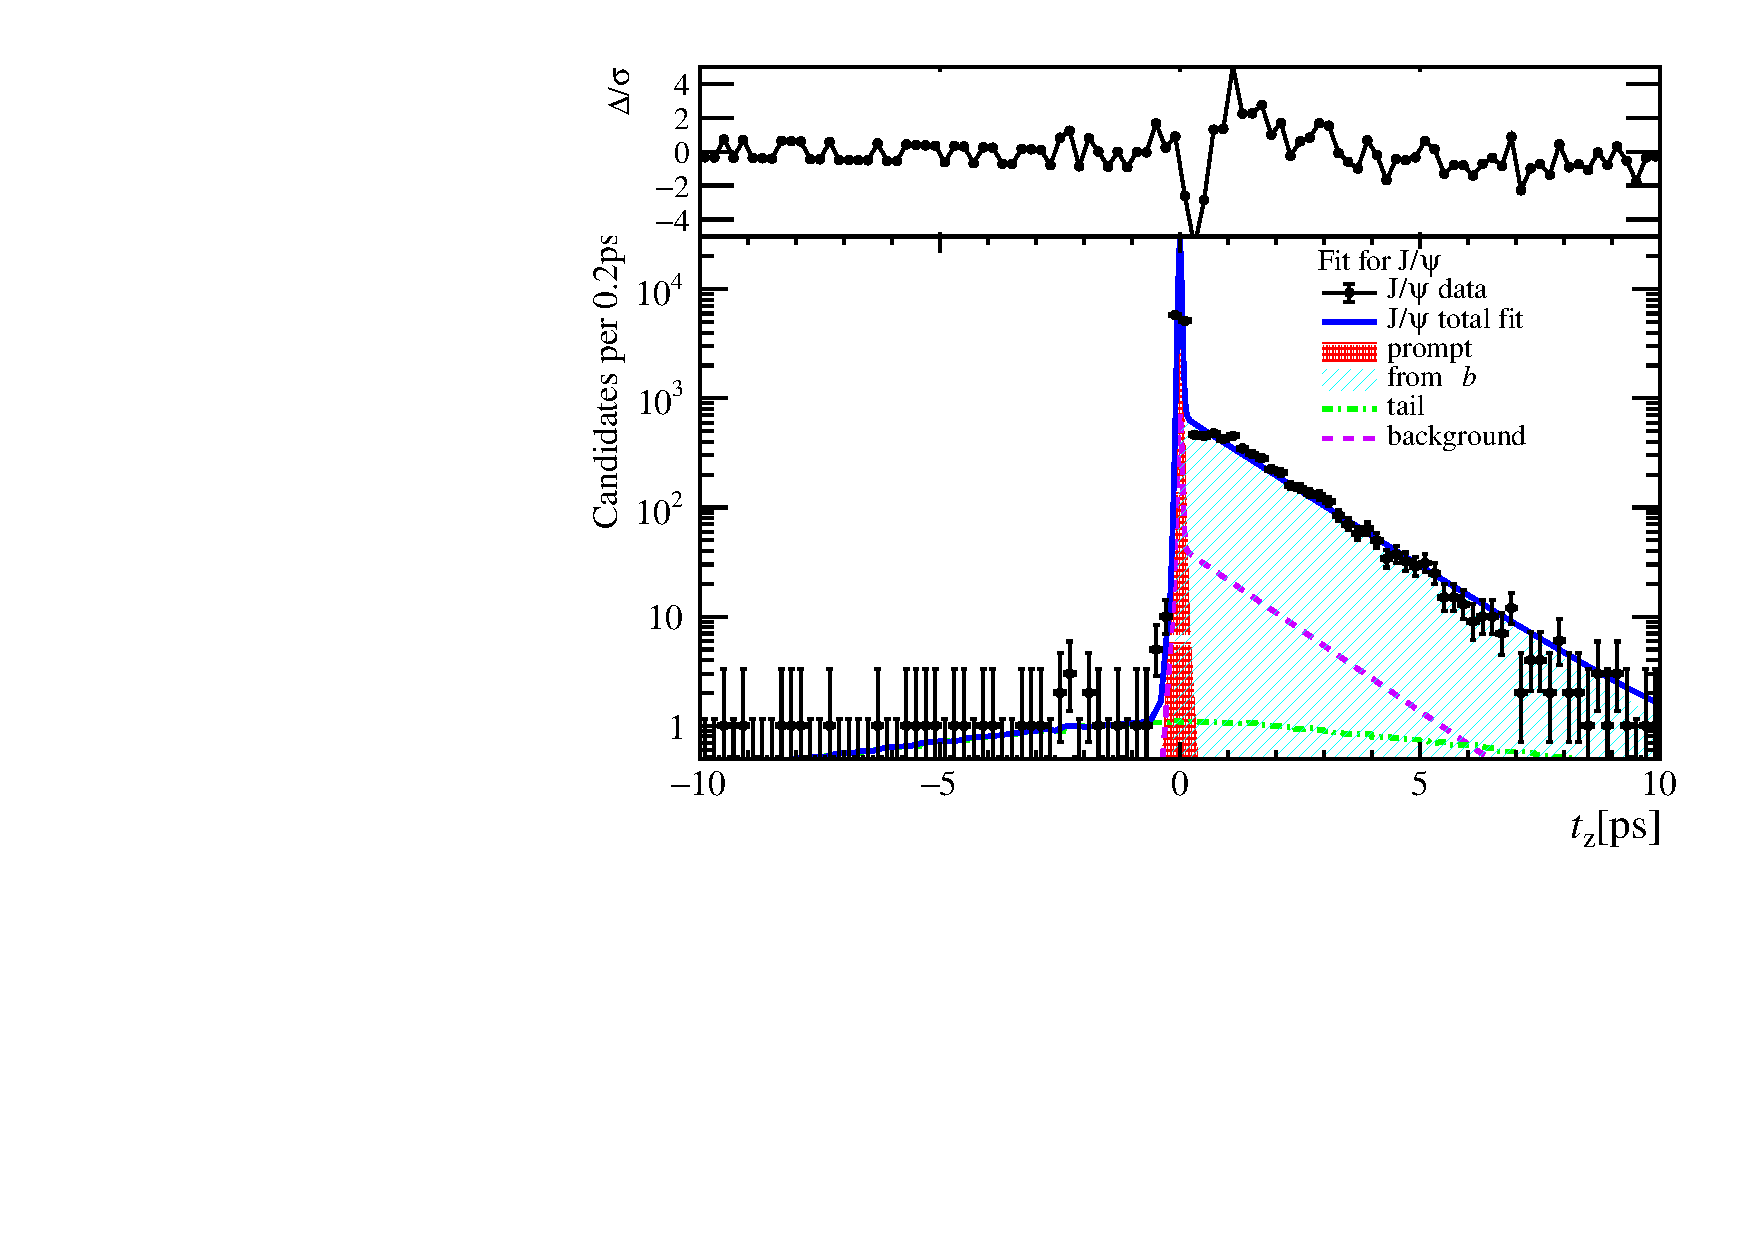
\includegraphics[width=0.47\linewidth]{pdf/Jpsi/2DFitF/n1y2pt5.pdf}
\vspace*{-0.5cm}
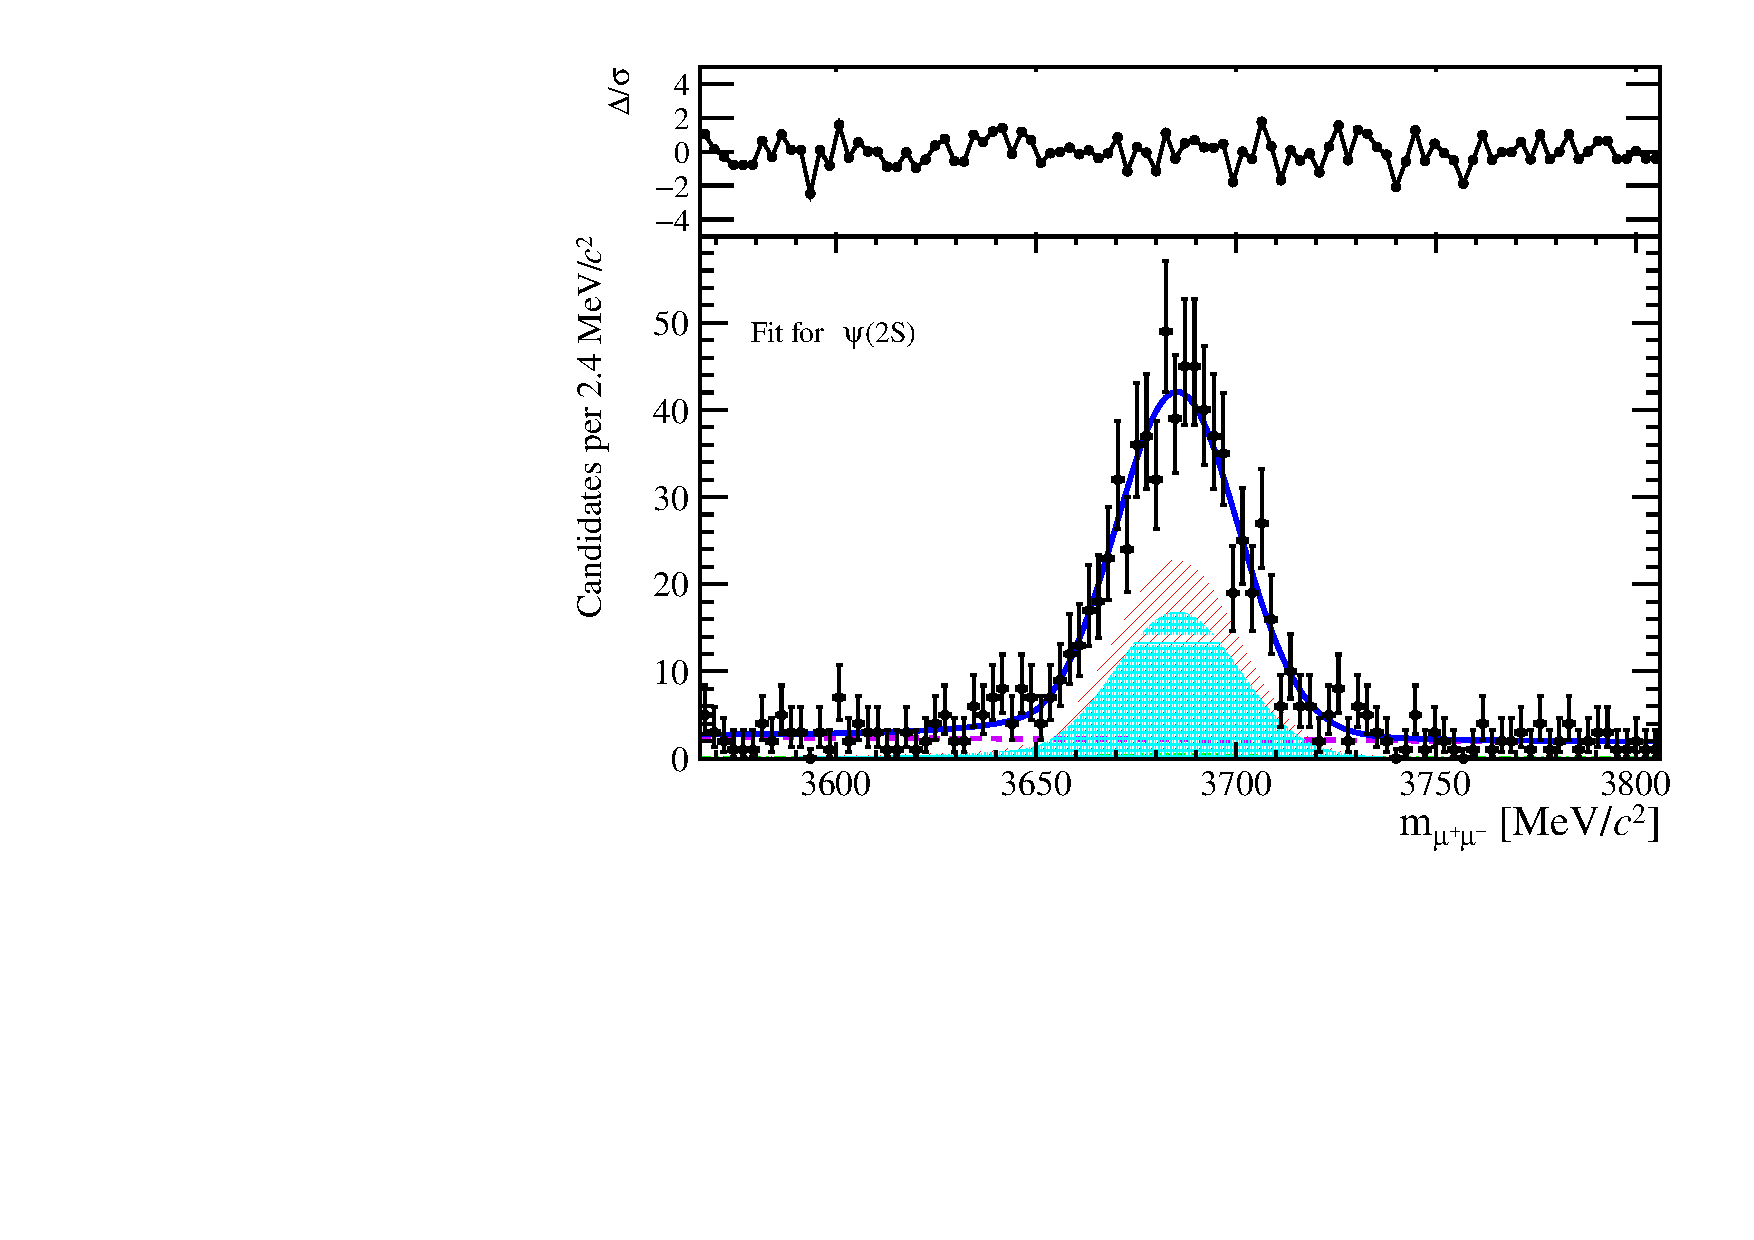
\includegraphics[width=0.47\linewidth]{pdf/Psi2S/drawmassF/n1y2pt5.pdf}
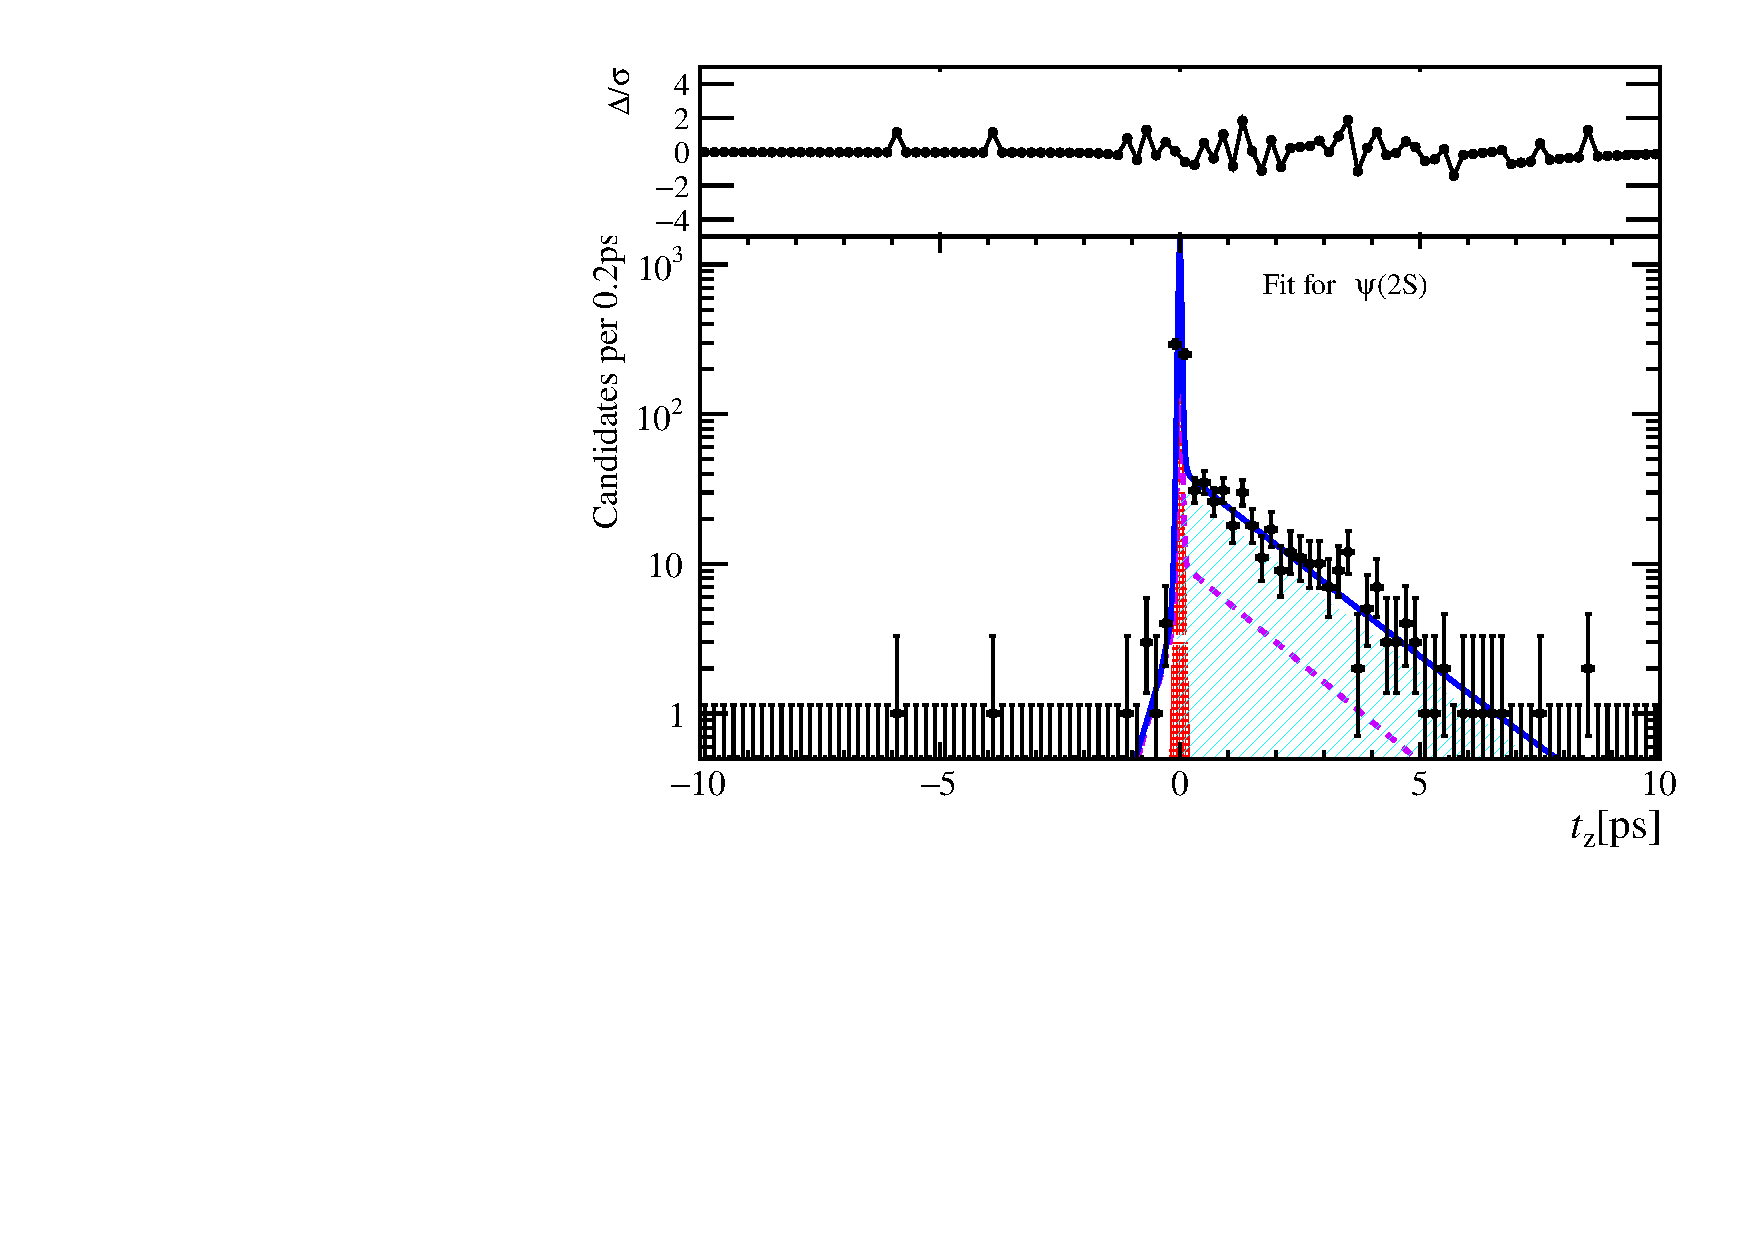
\includegraphics[width=0.47\linewidth]{pdf/Psi2S/2DFitF/n1y2pt5.pdf}
\vspace*{-0.5cm}
\end{center}
\caption{Fit results in $8\gevc<\pt<20\gevc$, $2.8<y<3.5$ and 0$\leq$nForwardTracks$<$12.}
\label{Fitn1y2pt5}
\end{figure}
\begin{figure}[H]
\begin{center}
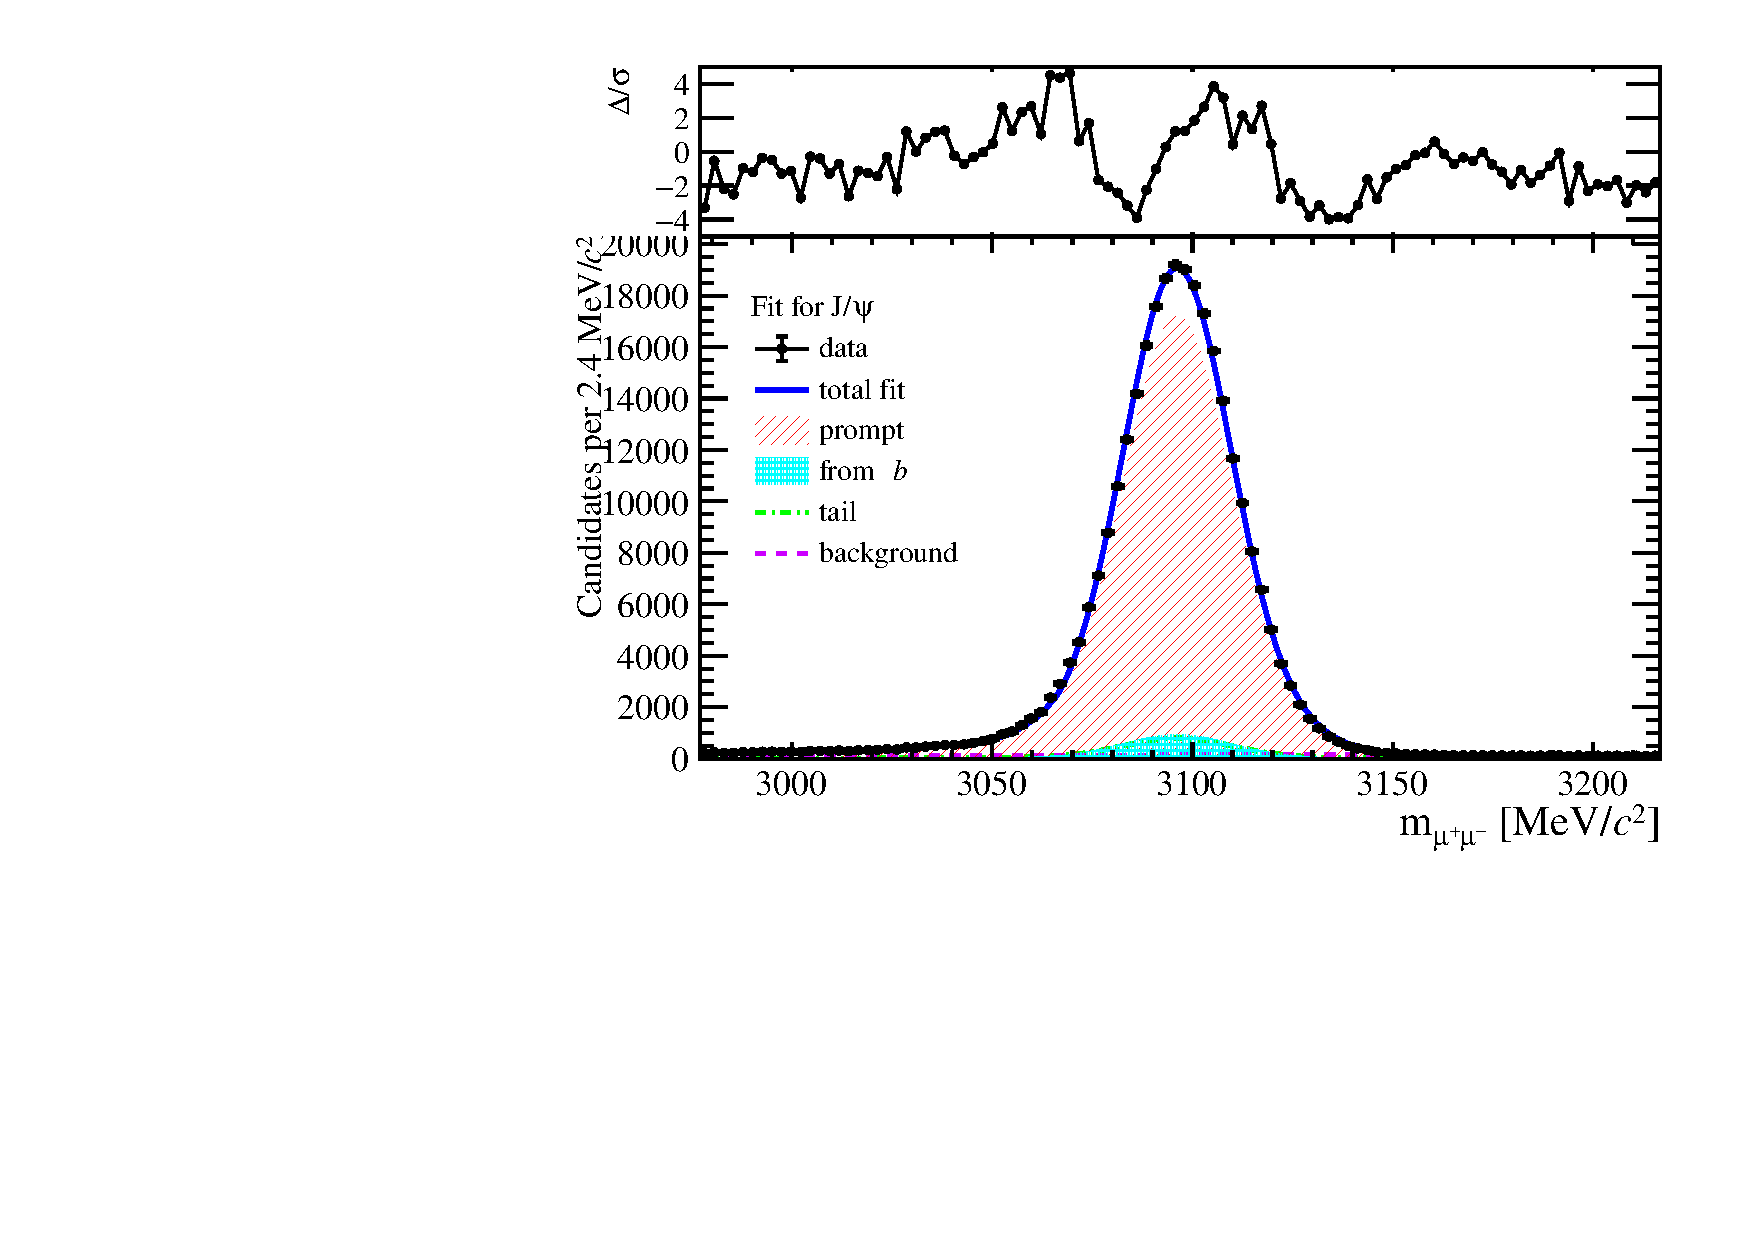
\includegraphics[width=0.47\linewidth]{pdf/Jpsi/drawmassF/n1y3pt1.pdf}
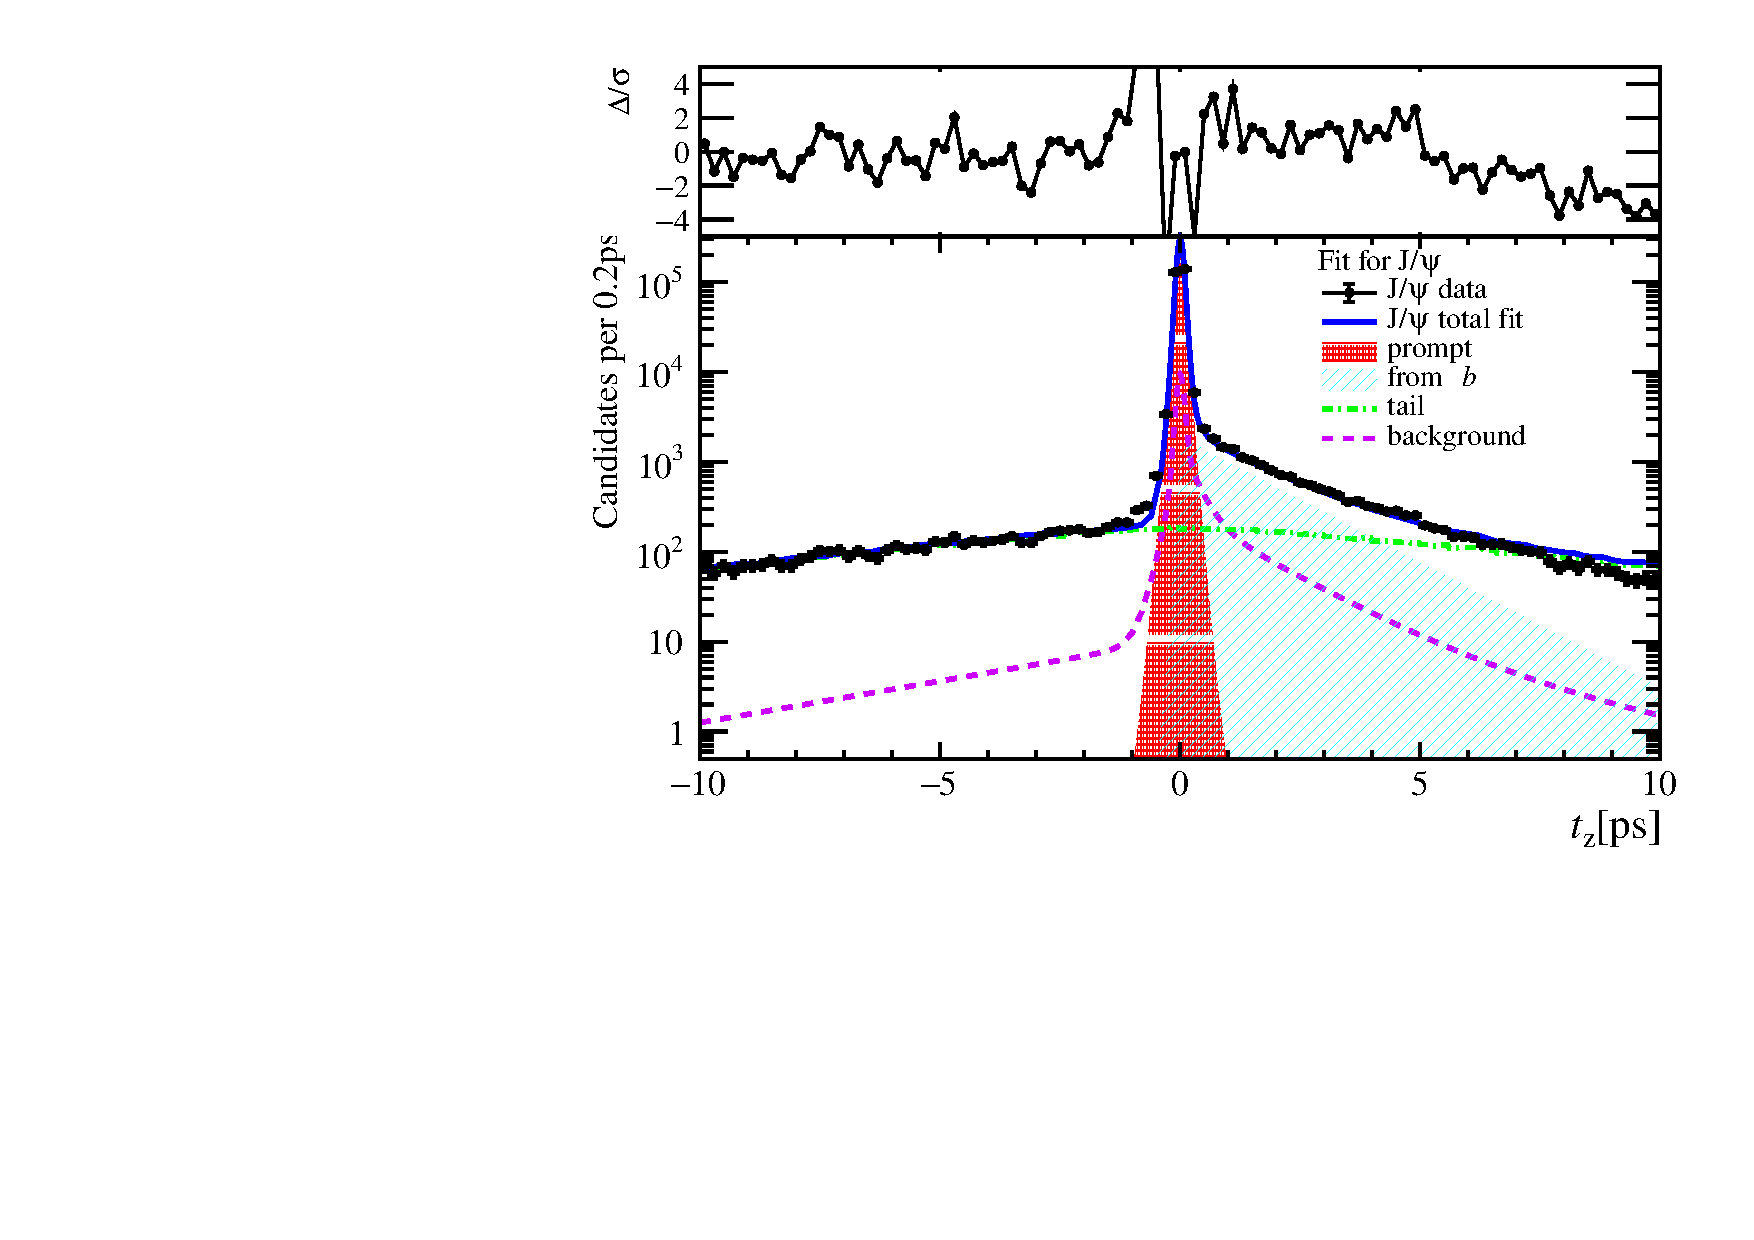
\includegraphics[width=0.47\linewidth]{pdf/Jpsi/2DFitF/n1y3pt1.pdf}
\vspace*{-0.5cm}
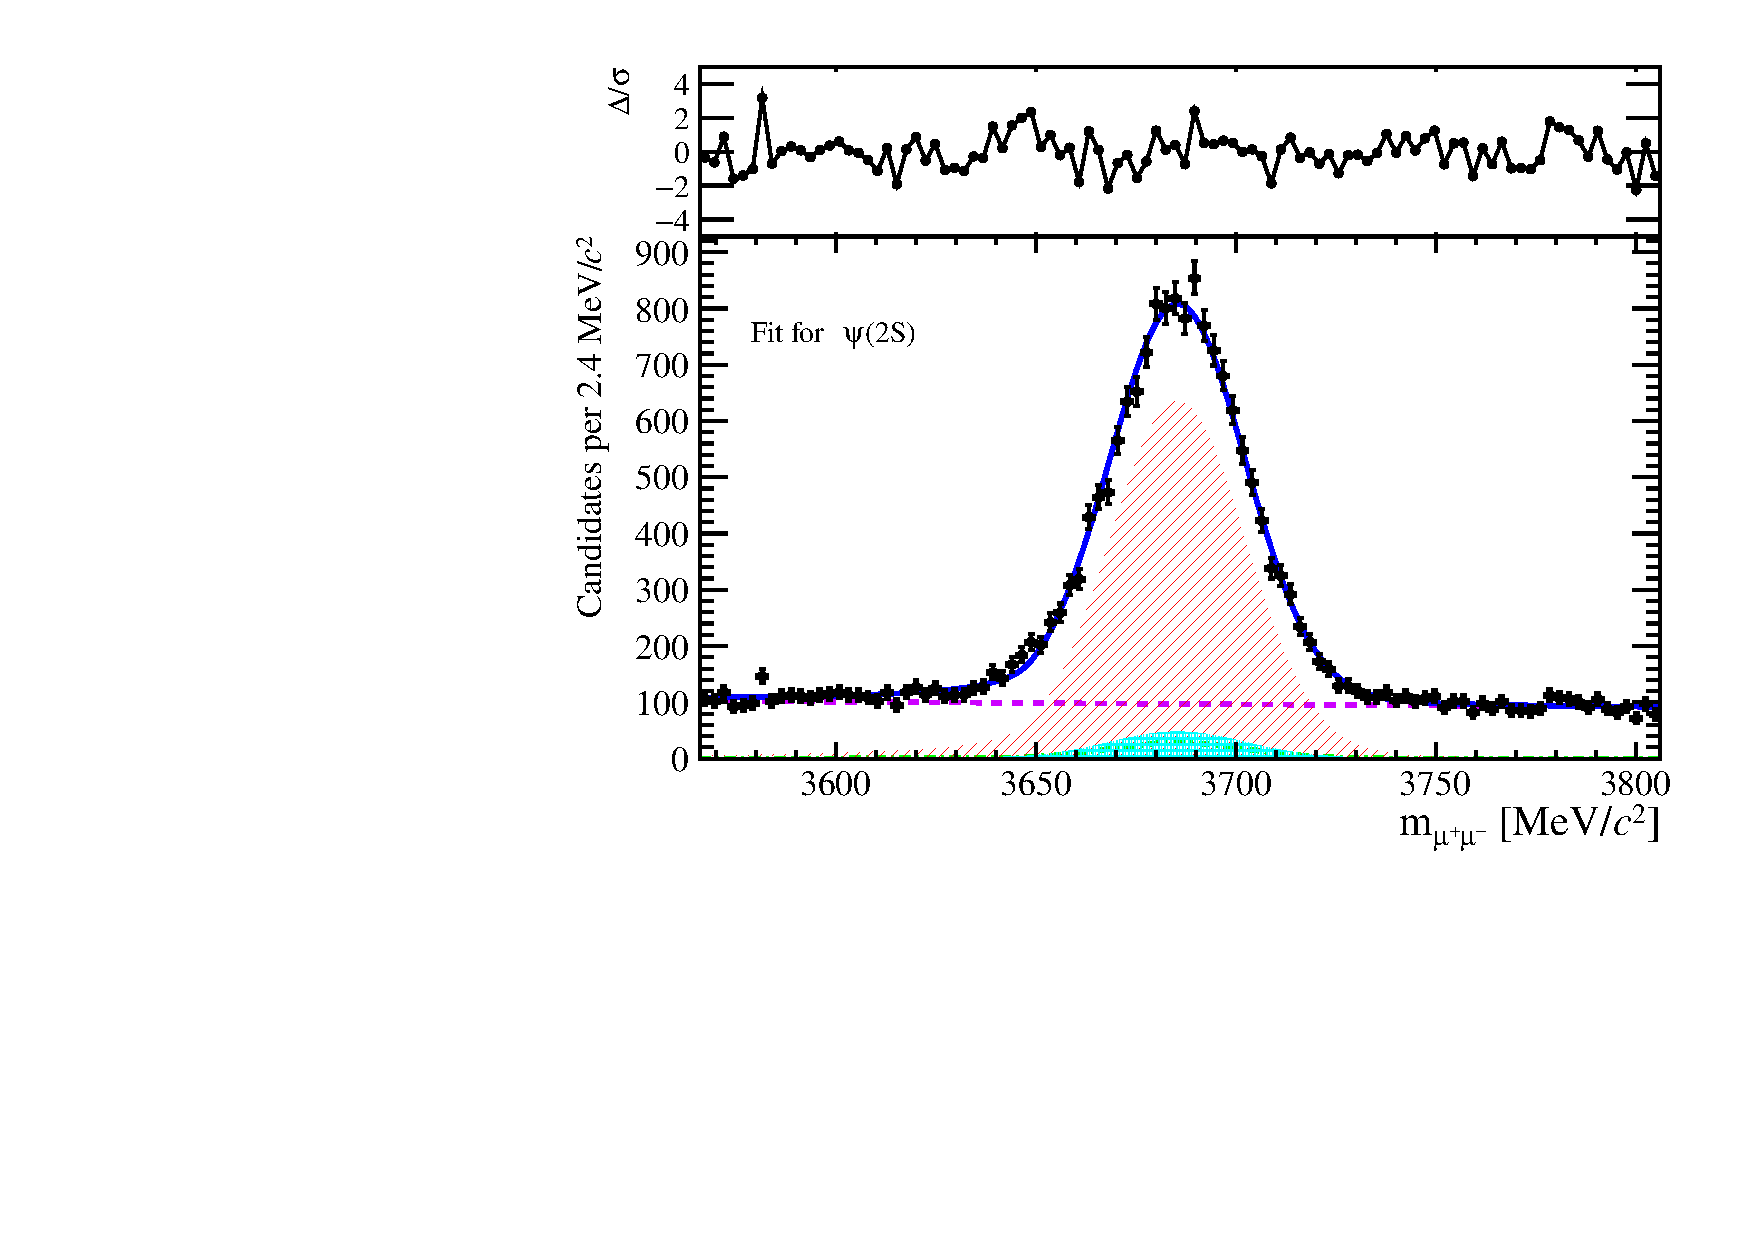
\includegraphics[width=0.47\linewidth]{pdf/Psi2S/drawmassF/n1y3pt1.pdf}
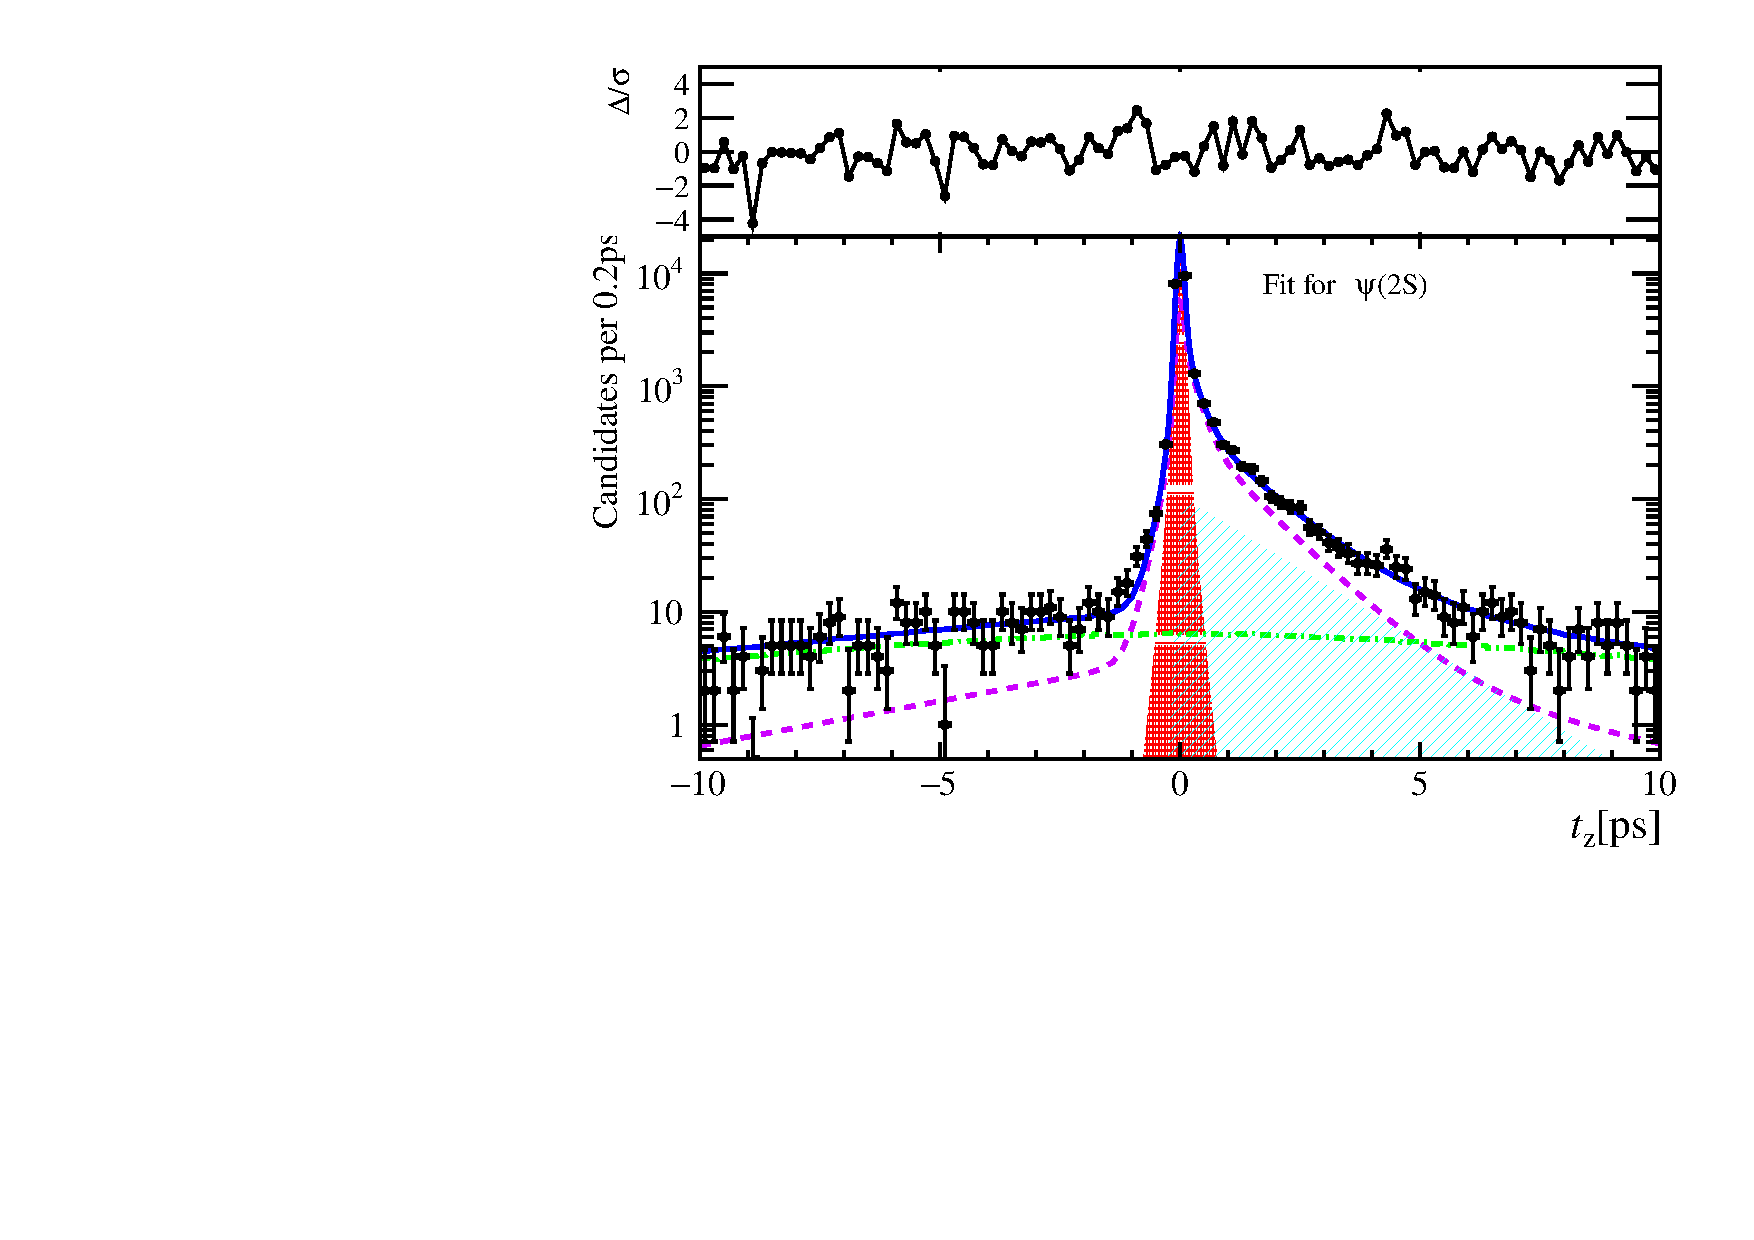
\includegraphics[width=0.47\linewidth]{pdf/Psi2S/2DFitF/n1y3pt1.pdf}
\vspace*{-0.5cm}
\end{center}
\caption{Fit results in $0\gevc<\pt<2\gevc$, $3.5<y<4.5$ and 0$\leq$nForwardTracks$<$12.}
\label{Fitn1y3pt1}
\end{figure}
\begin{figure}[H]
\begin{center}
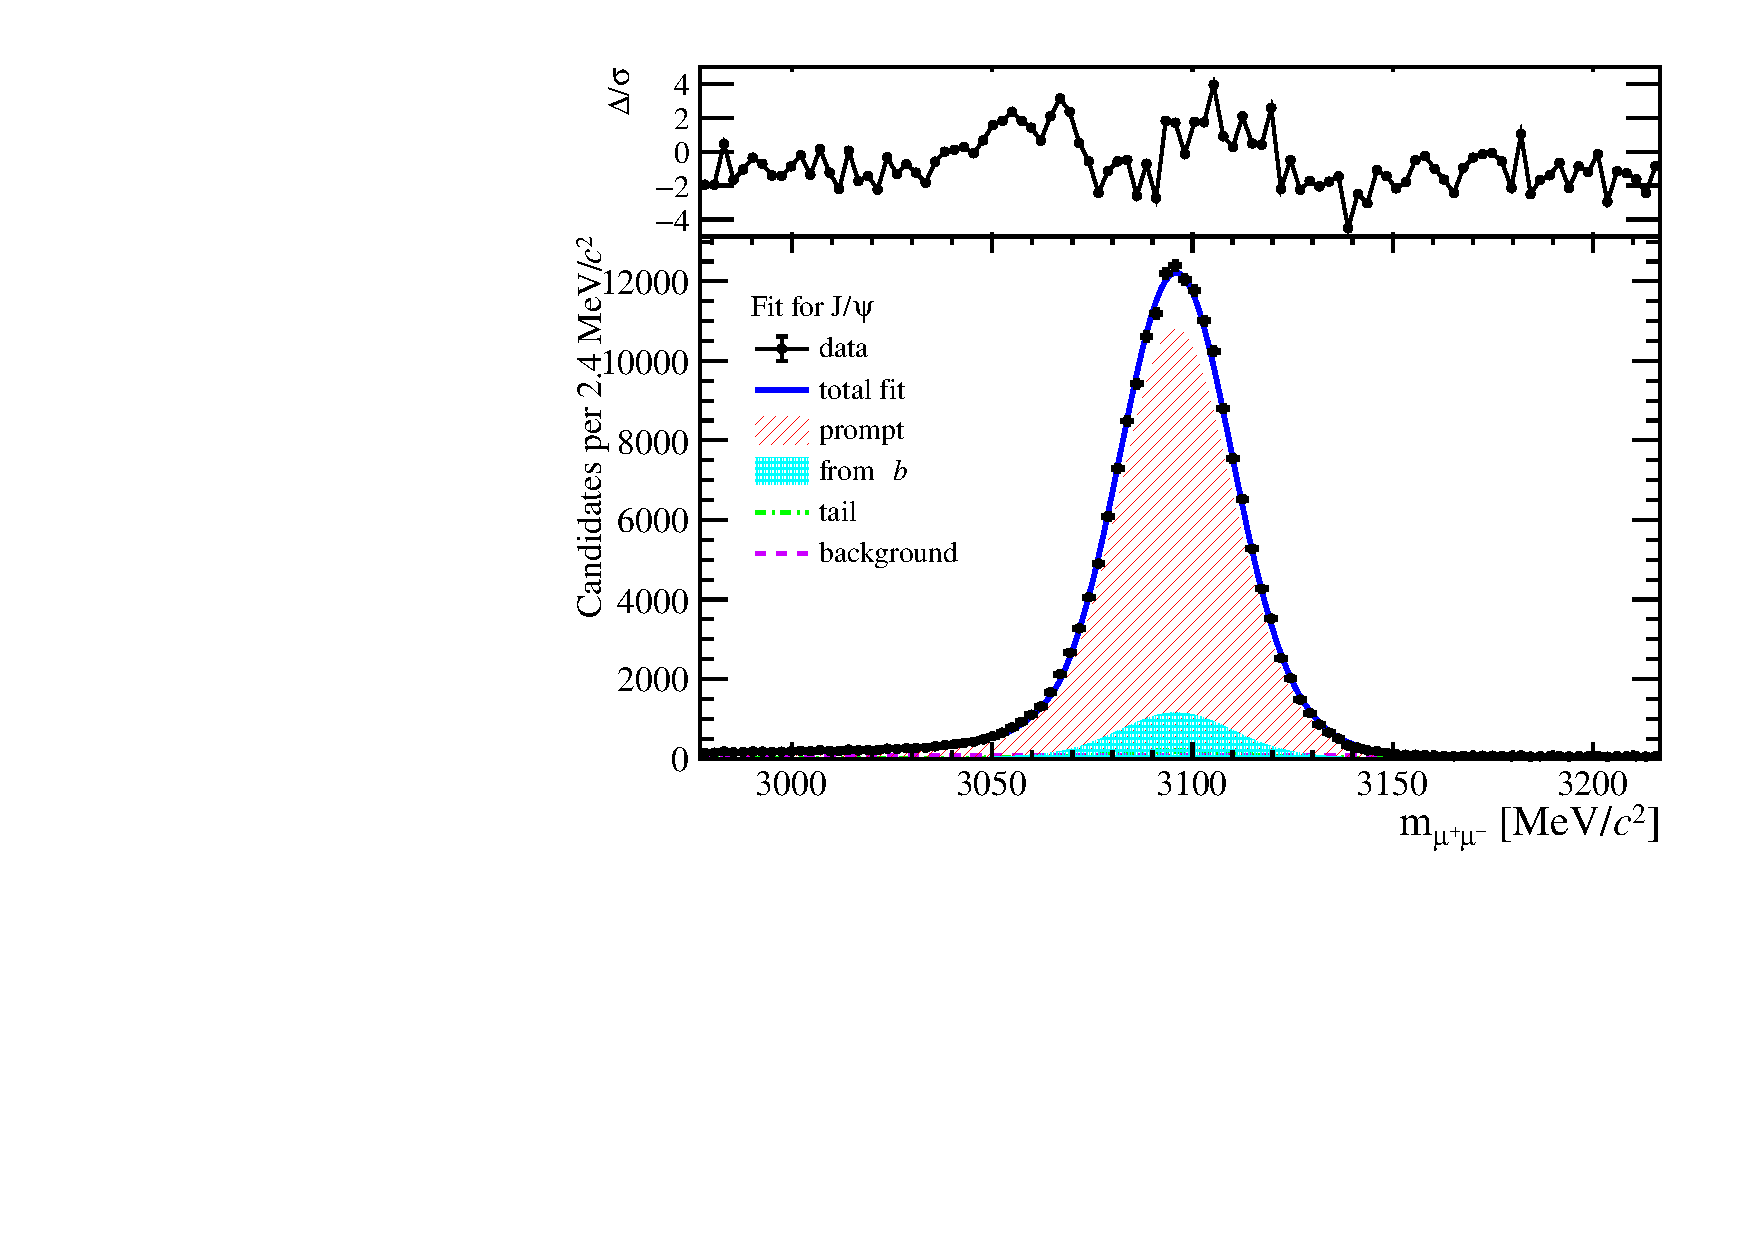
\includegraphics[width=0.47\linewidth]{pdf/Jpsi/drawmassF/n1y3pt2.pdf}
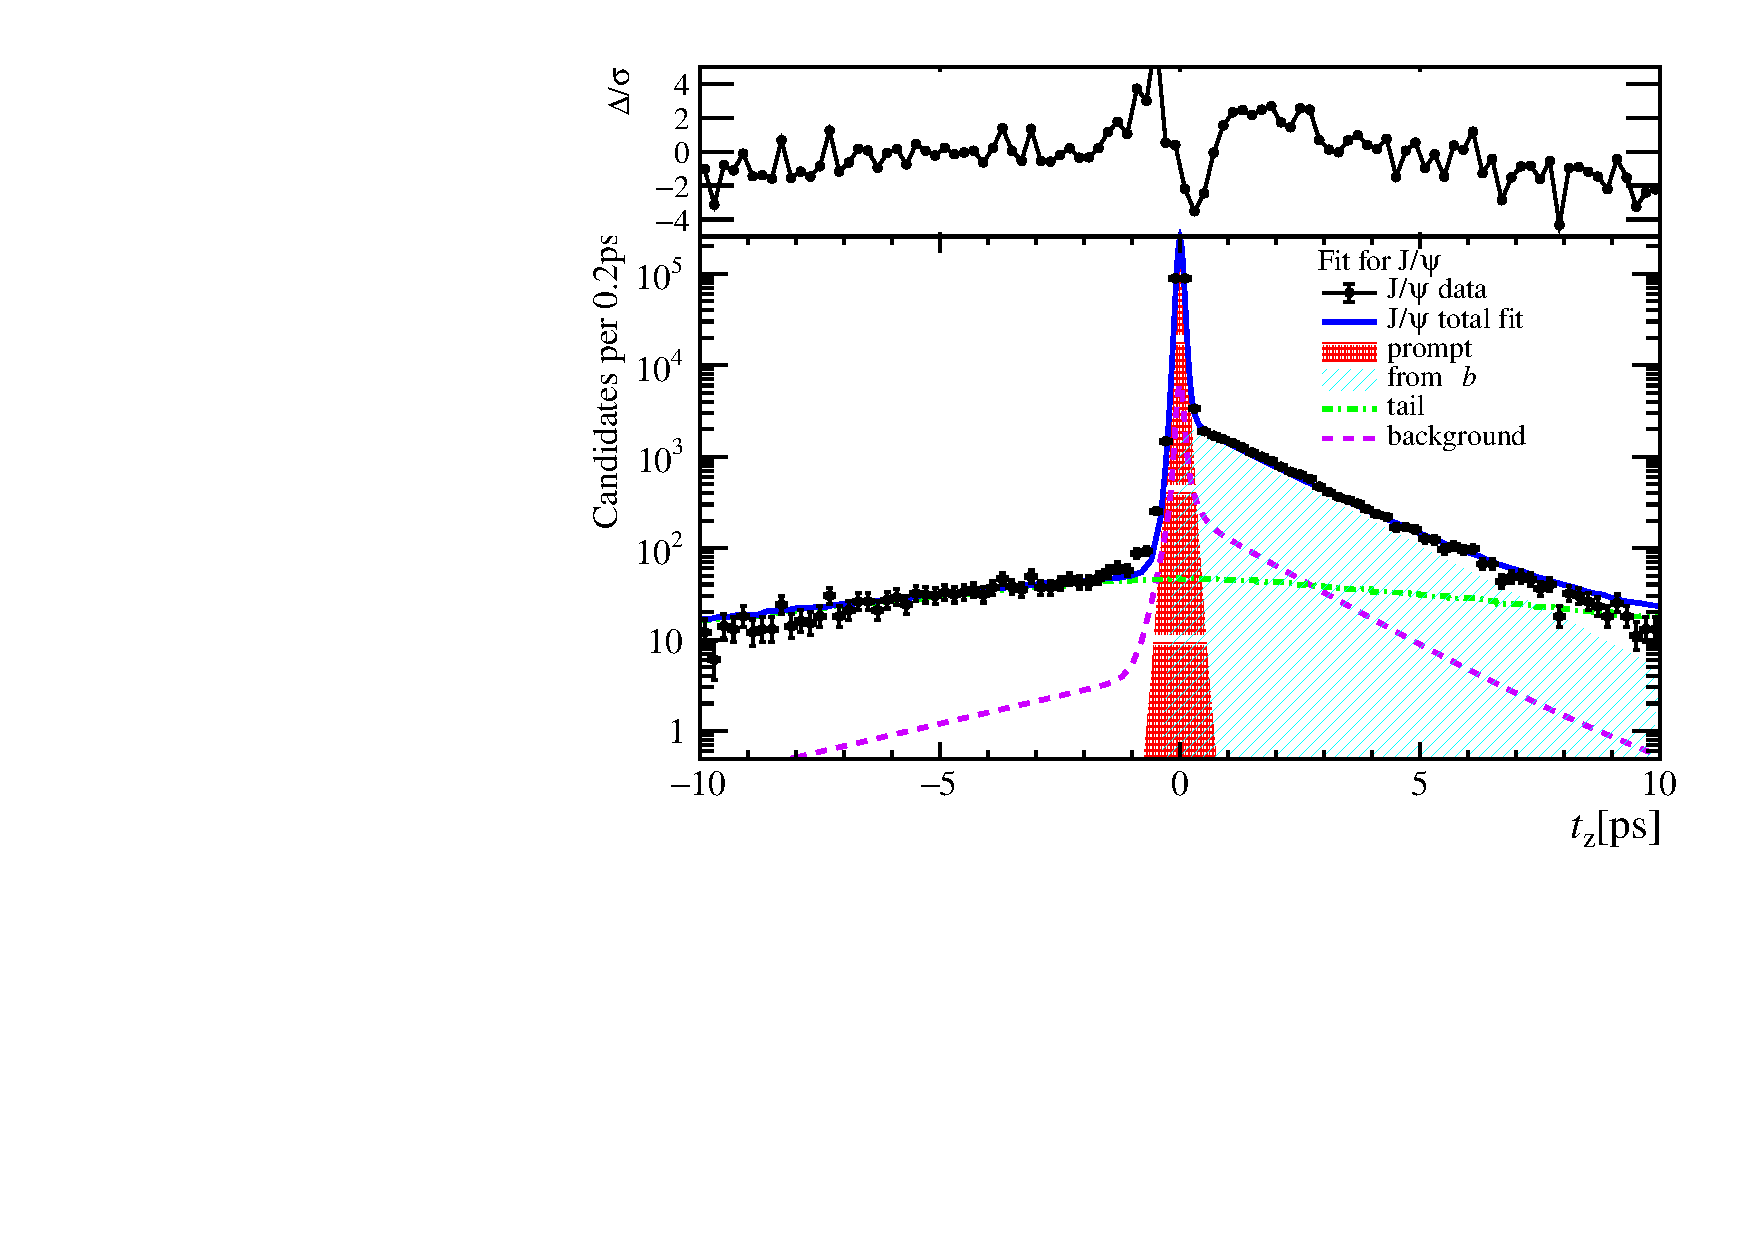
\includegraphics[width=0.47\linewidth]{pdf/Jpsi/2DFitF/n1y3pt2.pdf}
\vspace*{-0.5cm}
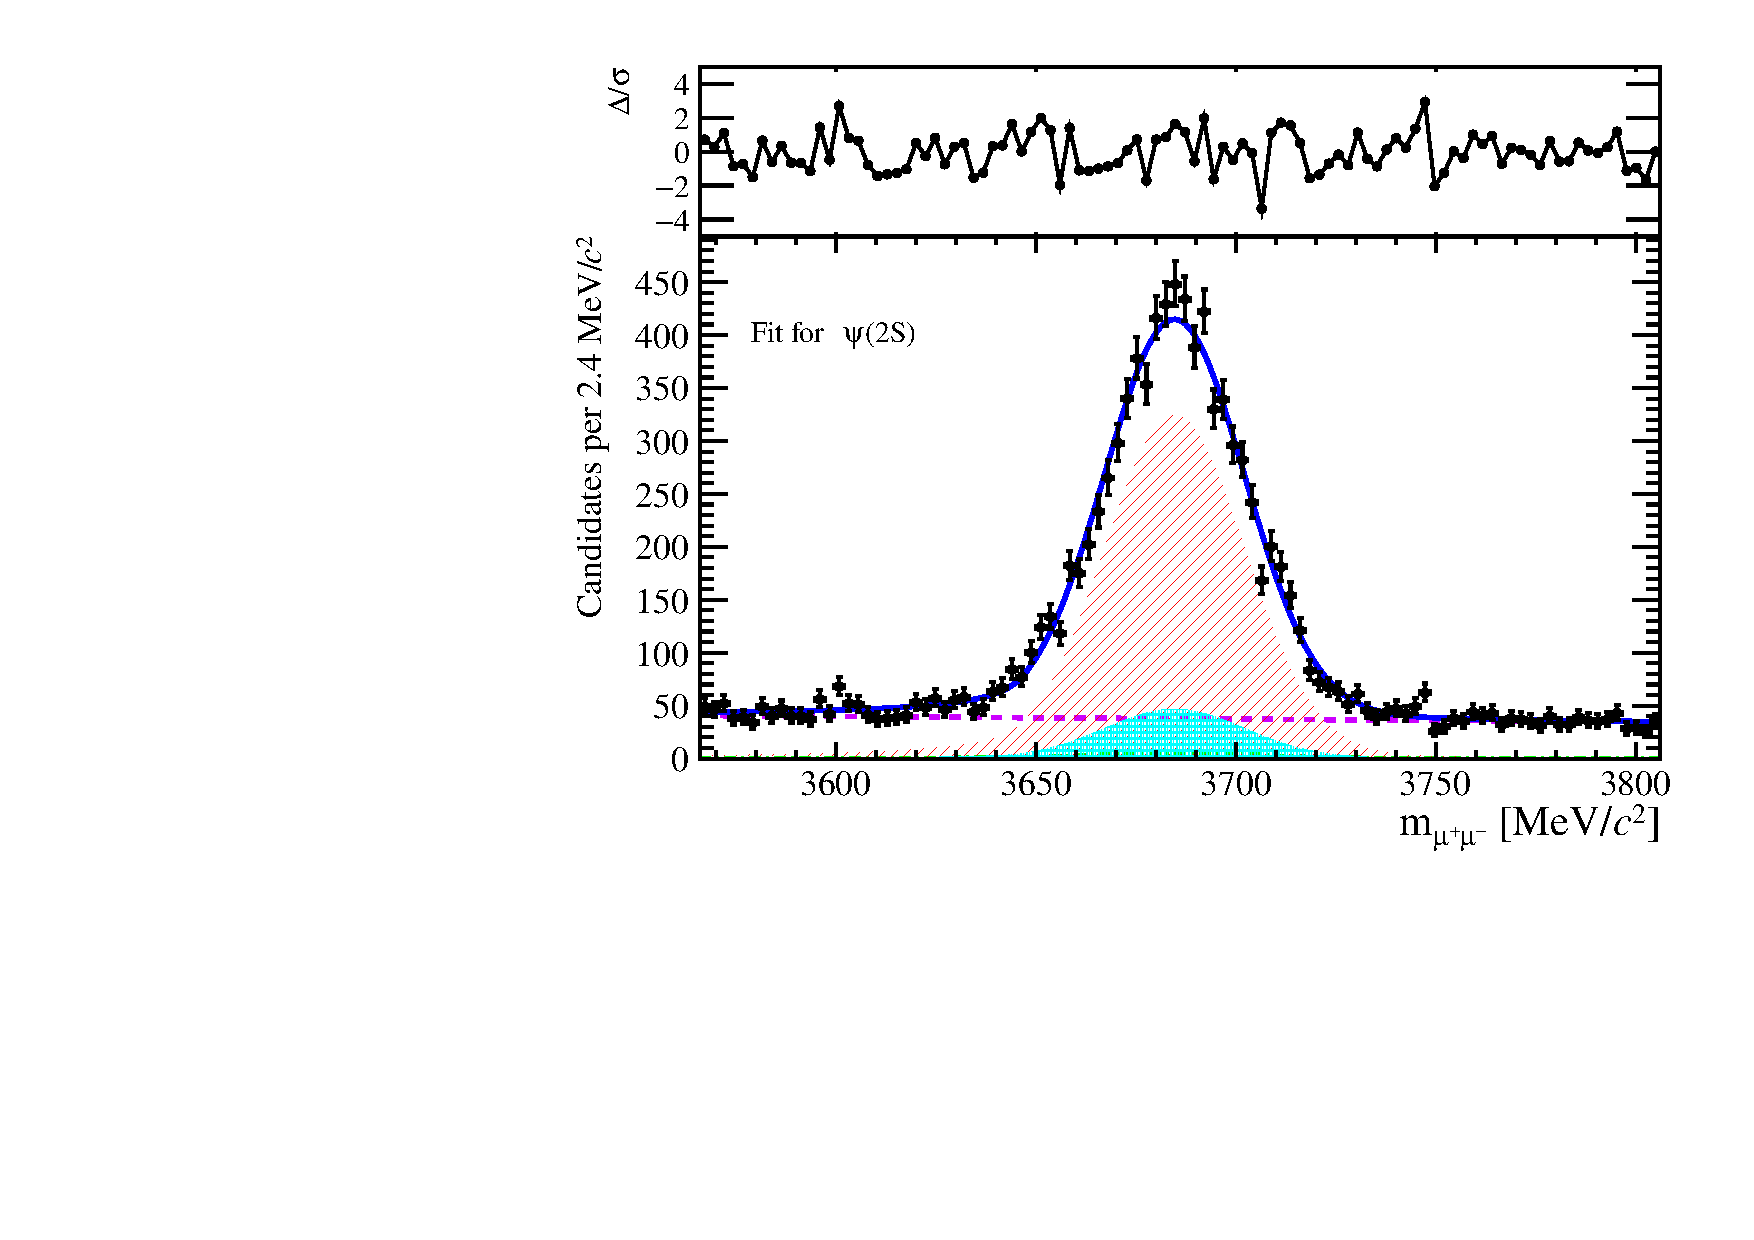
\includegraphics[width=0.47\linewidth]{pdf/Psi2S/drawmassF/n1y3pt2.pdf}
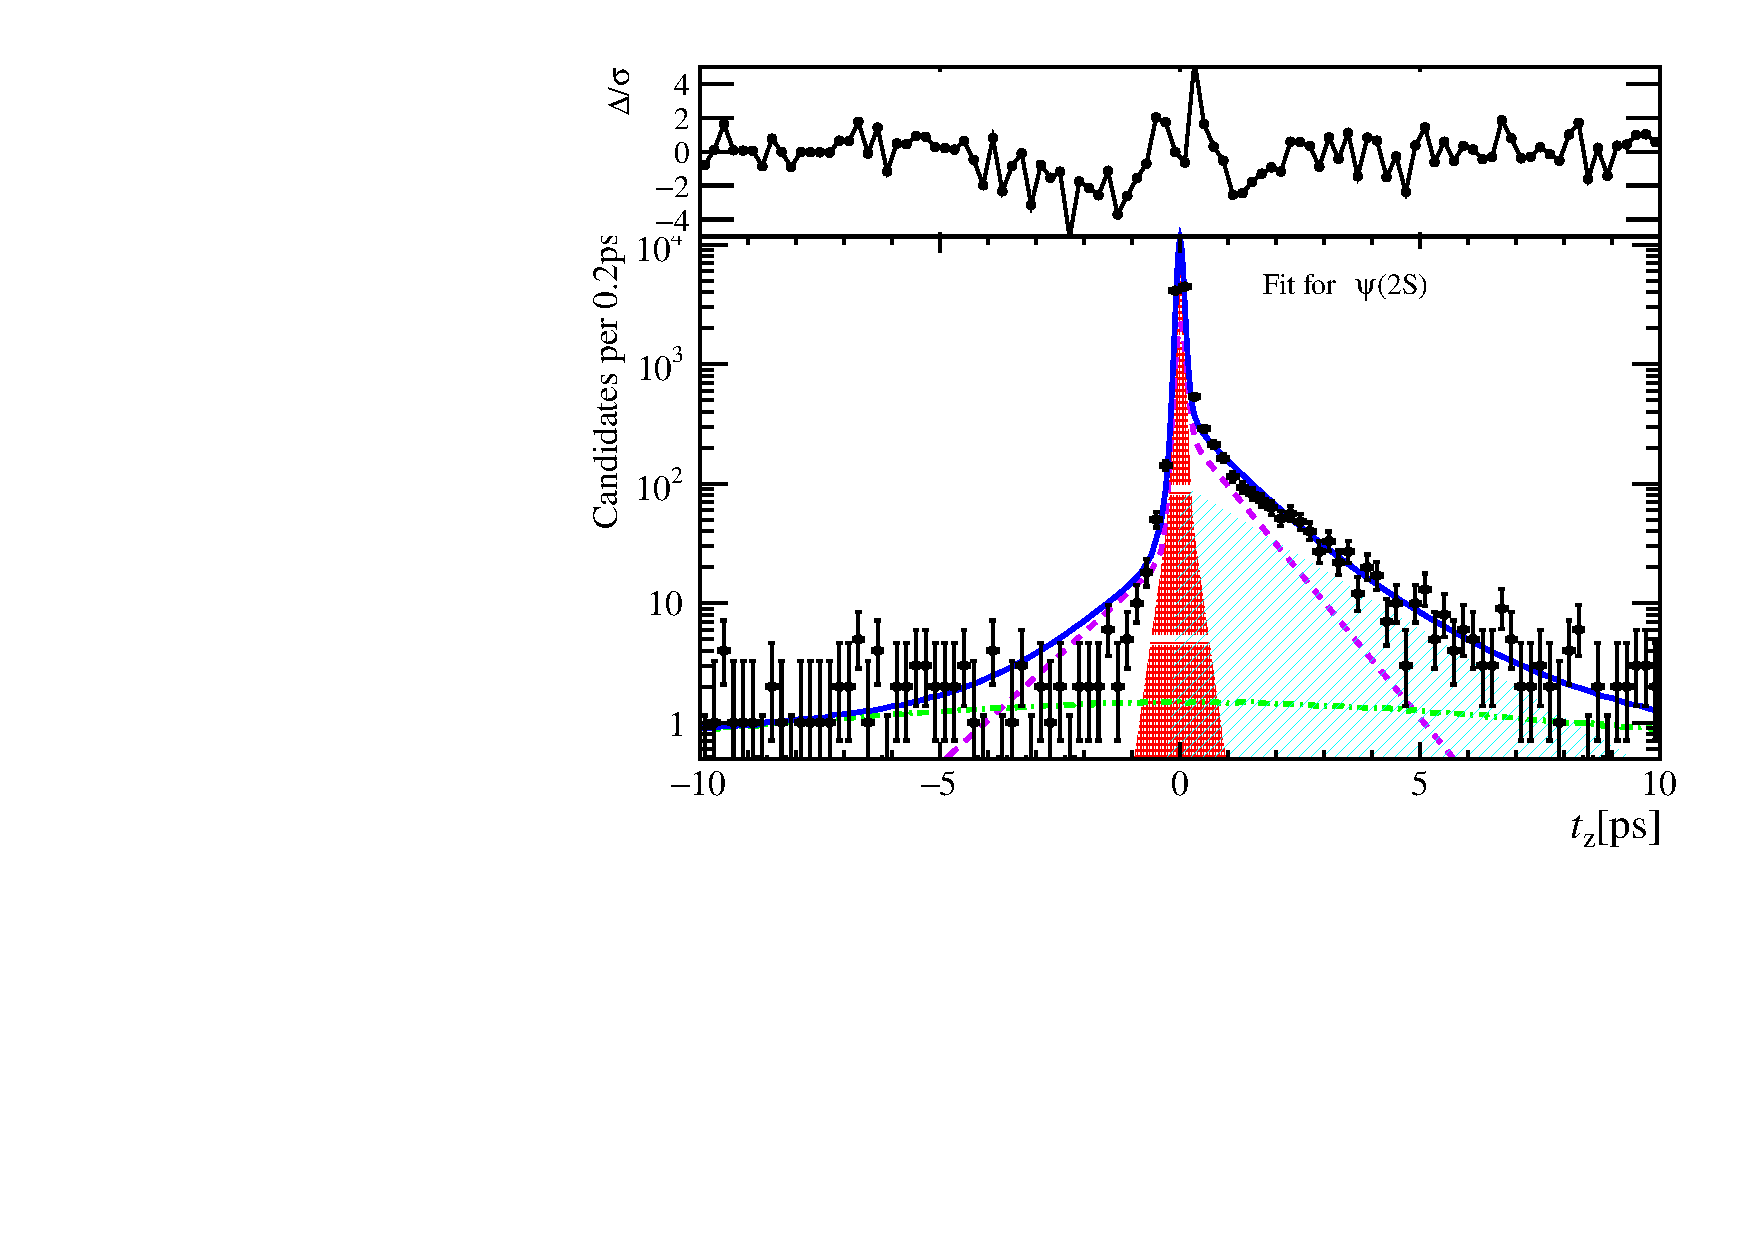
\includegraphics[width=0.47\linewidth]{pdf/Psi2S/2DFitF/n1y3pt2.pdf}
\vspace*{-0.5cm}
\end{center}
\caption{Fit results in $2\gevc<\pt<4\gevc$, $3.5<y<4.5$ and 0$\leq$nForwardTracks$<$12.}
\label{Fitn1y3pt2}
\end{figure}
\begin{figure}[H]
\begin{center}
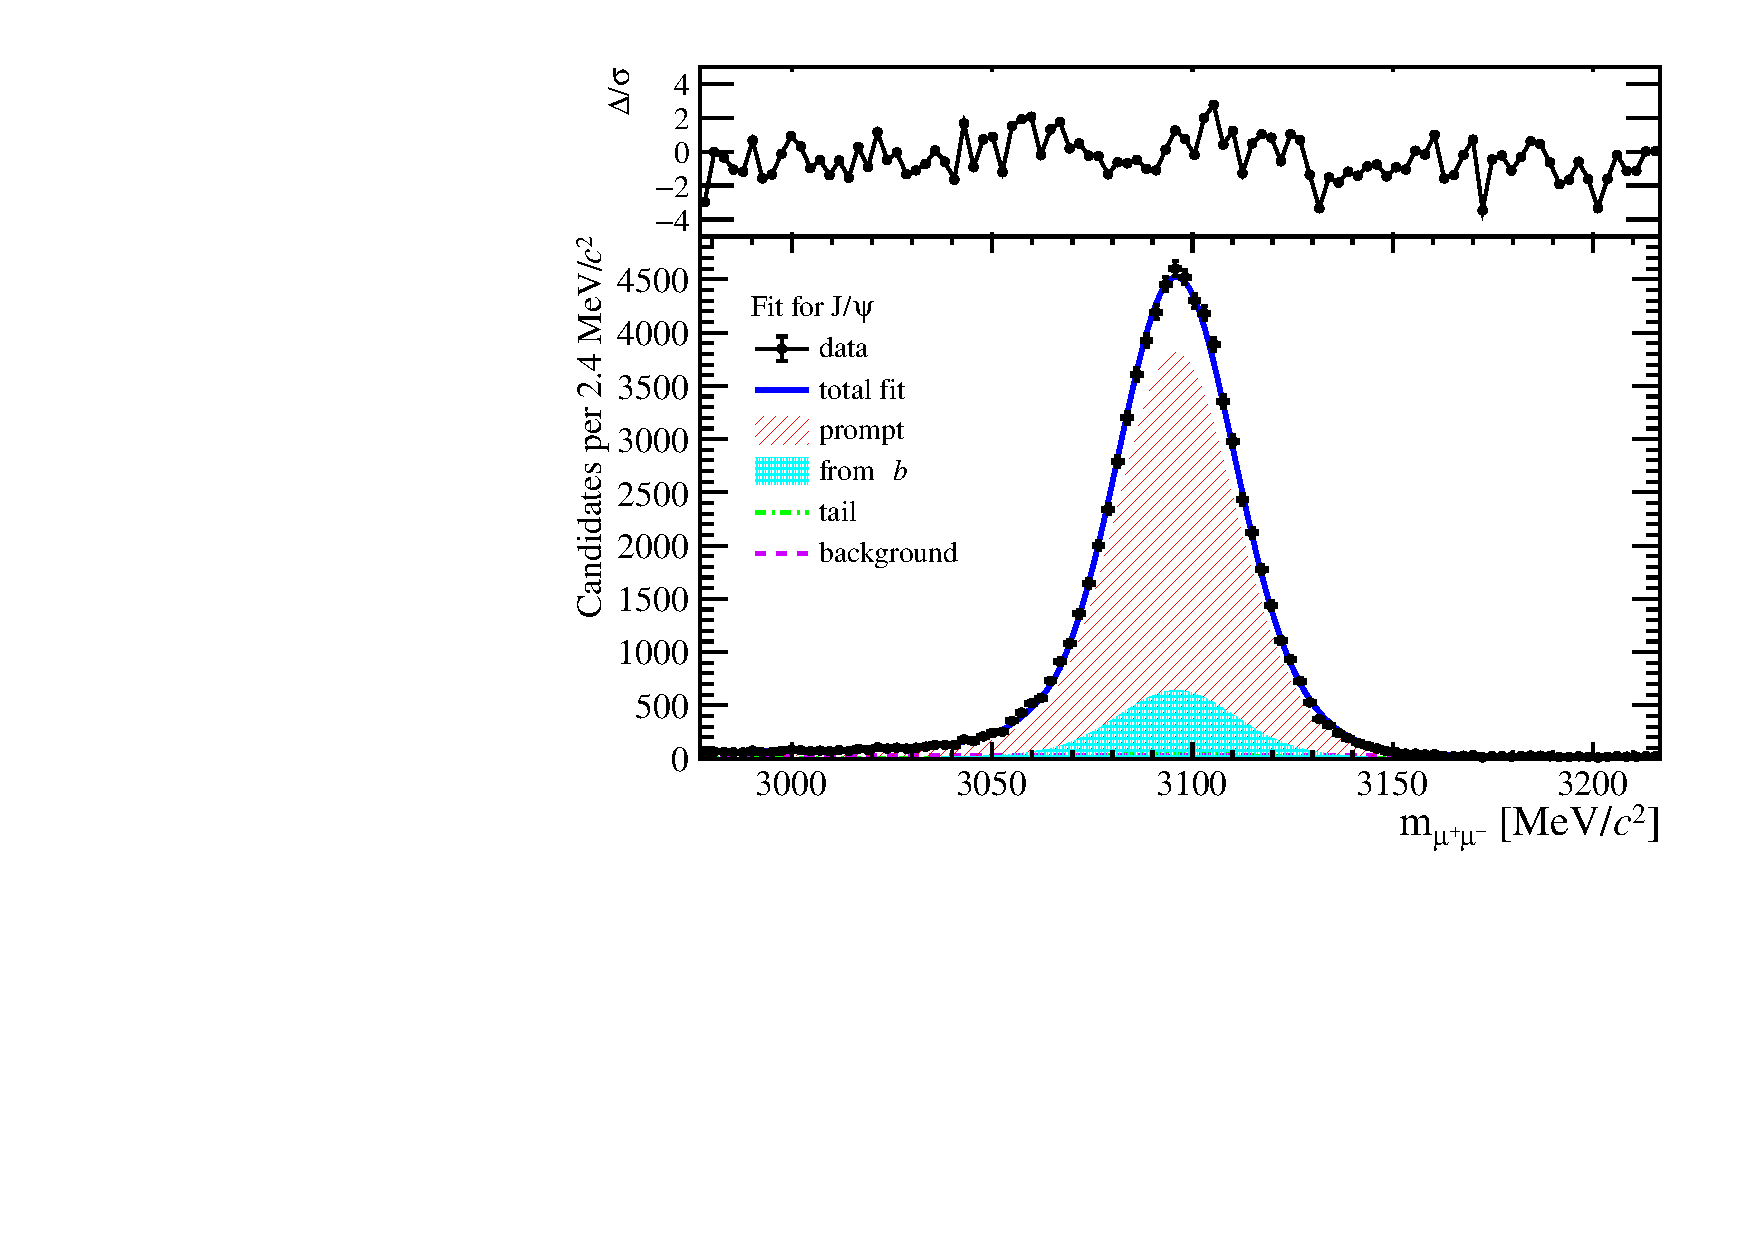
\includegraphics[width=0.47\linewidth]{pdf/Jpsi/drawmassF/n1y3pt3.pdf}
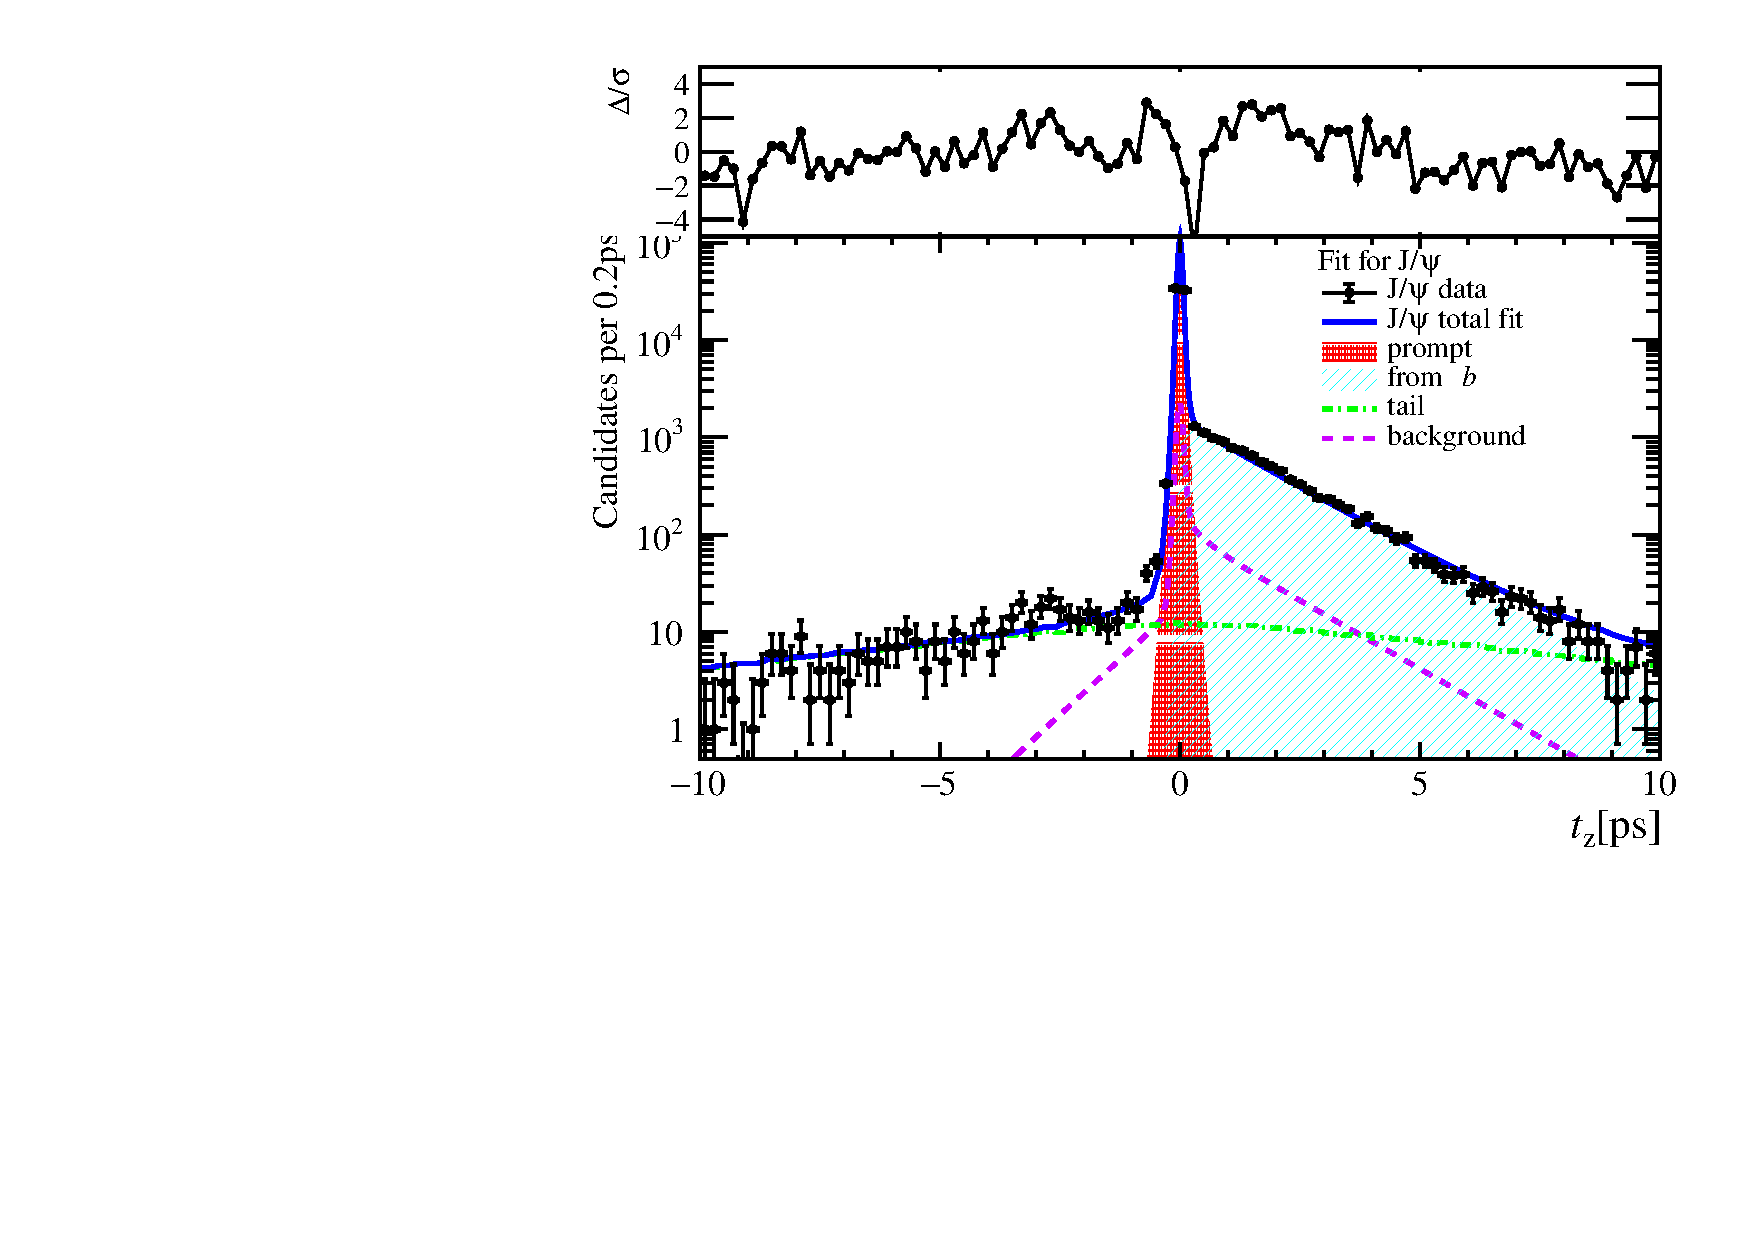
\includegraphics[width=0.47\linewidth]{pdf/Jpsi/2DFitF/n1y3pt3.pdf}
\vspace*{-0.5cm}
\includegraphics[width=0.47\linewidth]{pdf/Psi2S/drawmassF/n1y3pt3.pdf}
\includegraphics[width=0.47\linewidth]{pdf/Psi2S/2DFitF/n1y3pt3.pdf}
\vspace*{-0.5cm}
\end{center}
\caption{Fit results in $4\gevc<\pt<6\gevc$, $3.5<y<4.5$ and 0$\leq$nForwardTracks$<$12.}
\label{Fitn1y3pt3}
\end{figure}
\begin{figure}[H]
\begin{center}
\includegraphics[width=0.47\linewidth]{pdf/Jpsi/drawmassF/n1y3pt4.pdf}
\includegraphics[width=0.47\linewidth]{pdf/Jpsi/2DFitF/n1y3pt4.pdf}
\vspace*{-0.5cm}
\includegraphics[width=0.47\linewidth]{pdf/Psi2S/drawmassF/n1y3pt4.pdf}
\includegraphics[width=0.47\linewidth]{pdf/Psi2S/2DFitF/n1y3pt4.pdf}
\vspace*{-0.5cm}
\end{center}
\caption{Fit results in $6\gevc<\pt<8\gevc$, $3.5<y<4.5$ and 0$\leq$nForwardTracks$<$12.}
\label{Fitn1y3pt4}
\end{figure}
\begin{figure}[H]
\begin{center}
\includegraphics[width=0.47\linewidth]{pdf/Jpsi/drawmassF/n1y3pt5.pdf}
\includegraphics[width=0.47\linewidth]{pdf/Jpsi/2DFitF/n1y3pt5.pdf}
\vspace*{-0.5cm}
\includegraphics[width=0.47\linewidth]{pdf/Psi2S/drawmassF/n1y3pt5.pdf}
\includegraphics[width=0.47\linewidth]{pdf/Psi2S/2DFitF/n1y3pt5.pdf}
\vspace*{-0.5cm}
\end{center}
\caption{Fit results in $8\gevc<\pt<20\gevc$, $3.5<y<4.5$ and 0$\leq$nForwardTracks$<$12.}
\label{Fitn1y3pt5}
\end{figure}
\begin{figure}[H]
\begin{center}
\includegraphics[width=0.47\linewidth]{pdf/Jpsi/drawmassF/n2y1pt1.pdf}
\includegraphics[width=0.47\linewidth]{pdf/Jpsi/2DFitF/n2y1pt1.pdf}
\vspace*{-0.5cm}
\includegraphics[width=0.47\linewidth]{pdf/Psi2S/drawmassF/n2y1pt1.pdf}
\includegraphics[width=0.47\linewidth]{pdf/Psi2S/2DFitF/n2y1pt1.pdf}
\vspace*{-0.5cm}
\end{center}
\caption{Fit results in $0\gevc<\pt<2\gevc$, $2.0<y<2.8$ and 12$\leq$nForwardTracks$<$24.}
\label{Fitn2y1pt1}
\end{figure}
\begin{figure}[H]
\begin{center}
\includegraphics[width=0.47\linewidth]{pdf/Jpsi/drawmassF/n2y1pt2.pdf}
\includegraphics[width=0.47\linewidth]{pdf/Jpsi/2DFitF/n2y1pt2.pdf}
\vspace*{-0.5cm}
\includegraphics[width=0.47\linewidth]{pdf/Psi2S/drawmassF/n2y1pt2.pdf}
\includegraphics[width=0.47\linewidth]{pdf/Psi2S/2DFitF/n2y1pt2.pdf}
\vspace*{-0.5cm}
\end{center}
\caption{Fit results in $2\gevc<\pt<4\gevc$, $2.0<y<2.8$ and 12$\leq$nForwardTracks$<$24.}
\label{Fitn2y1pt2}
\end{figure}
\begin{figure}[H]
\begin{center}
\includegraphics[width=0.47\linewidth]{pdf/Jpsi/drawmassF/n2y1pt3.pdf}
\includegraphics[width=0.47\linewidth]{pdf/Jpsi/2DFitF/n2y1pt3.pdf}
\vspace*{-0.5cm}
\includegraphics[width=0.47\linewidth]{pdf/Psi2S/drawmassF/n2y1pt3.pdf}
\includegraphics[width=0.47\linewidth]{pdf/Psi2S/2DFitF/n2y1pt3.pdf}
\vspace*{-0.5cm}
\end{center}
\caption{Fit results in $4\gevc<\pt<6\gevc$, $2.0<y<2.8$ and 12$\leq$nForwardTracks$<$24.}
\label{Fitn2y1pt3}
\end{figure}
\begin{figure}[H]
\begin{center}
\includegraphics[width=0.47\linewidth]{pdf/Jpsi/drawmassF/n2y1pt4.pdf}
\includegraphics[width=0.47\linewidth]{pdf/Jpsi/2DFitF/n2y1pt4.pdf}
\vspace*{-0.5cm}
\includegraphics[width=0.47\linewidth]{pdf/Psi2S/drawmassF/n2y1pt4.pdf}
\includegraphics[width=0.47\linewidth]{pdf/Psi2S/2DFitF/n2y1pt4.pdf}
\vspace*{-0.5cm}
\end{center}
\caption{Fit results in $6\gevc<\pt<8\gevc$, $2.0<y<2.8$ and 12$\leq$nForwardTracks$<$24.}
\label{Fitn2y1pt4}
\end{figure}
\begin{figure}[H]
\begin{center}
\includegraphics[width=0.47\linewidth]{pdf/Jpsi/drawmassF/n2y1pt5.pdf}
\includegraphics[width=0.47\linewidth]{pdf/Jpsi/2DFitF/n2y1pt5.pdf}
\vspace*{-0.5cm}
\includegraphics[width=0.47\linewidth]{pdf/Psi2S/drawmassF/n2y1pt5.pdf}
\includegraphics[width=0.47\linewidth]{pdf/Psi2S/2DFitF/n2y1pt5.pdf}
\vspace*{-0.5cm}
\end{center}
\caption{Fit results in $8\gevc<\pt<20\gevc$, $2.0<y<2.8$ and 12$\leq$nForwardTracks$<$24.}
\label{Fitn2y1pt5}
\end{figure}
\begin{figure}[H]
\begin{center}
\includegraphics[width=0.47\linewidth]{pdf/Jpsi/drawmassF/n2y2pt1.pdf}
\includegraphics[width=0.47\linewidth]{pdf/Jpsi/2DFitF/n2y2pt1.pdf}
\vspace*{-0.5cm}
\includegraphics[width=0.47\linewidth]{pdf/Psi2S/drawmassF/n2y2pt1.pdf}
\includegraphics[width=0.47\linewidth]{pdf/Psi2S/2DFitF/n2y2pt1.pdf}
\vspace*{-0.5cm}
\end{center}
\caption{Fit results in $0\gevc<\pt<2\gevc$, $2.8<y<3.5$ and 12$\leq$nForwardTracks$<$24.}
\label{Fitn2y2pt1}
\end{figure}
\begin{figure}[H]
\begin{center}
\includegraphics[width=0.47\linewidth]{pdf/Jpsi/drawmassF/n2y2pt2.pdf}
\includegraphics[width=0.47\linewidth]{pdf/Jpsi/2DFitF/n2y2pt2.pdf}
\vspace*{-0.5cm}
\includegraphics[width=0.47\linewidth]{pdf/Psi2S/drawmassF/n2y2pt2.pdf}
\includegraphics[width=0.47\linewidth]{pdf/Psi2S/2DFitF/n2y2pt2.pdf}
\vspace*{-0.5cm}
\end{center}
\caption{Fit results in $2\gevc<\pt<4\gevc$, $2.8<y<3.5$ and 12$\leq$nForwardTracks$<$24.}
\label{Fitn2y2pt2}
\end{figure}
\begin{figure}[H]
\begin{center}
\includegraphics[width=0.47\linewidth]{pdf/Jpsi/drawmassF/n2y2pt3.pdf}
\includegraphics[width=0.47\linewidth]{pdf/Jpsi/2DFitF/n2y2pt3.pdf}
\vspace*{-0.5cm}
\includegraphics[width=0.47\linewidth]{pdf/Psi2S/drawmassF/n2y2pt3.pdf}
\includegraphics[width=0.47\linewidth]{pdf/Psi2S/2DFitF/n2y2pt3.pdf}
\vspace*{-0.5cm}
\end{center}
\caption{Fit results in $4\gevc<\pt<6\gevc$, $2.8<y<3.5$ and 12$\leq$nForwardTracks$<$24.}
\label{Fitn2y2pt3}
\end{figure}
\begin{figure}[H]
\begin{center}
\includegraphics[width=0.47\linewidth]{pdf/Jpsi/drawmassF/n2y2pt4.pdf}
\includegraphics[width=0.47\linewidth]{pdf/Jpsi/2DFitF/n2y2pt4.pdf}
\vspace*{-0.5cm}
\includegraphics[width=0.47\linewidth]{pdf/Psi2S/drawmassF/n2y2pt4.pdf}
\includegraphics[width=0.47\linewidth]{pdf/Psi2S/2DFitF/n2y2pt4.pdf}
\vspace*{-0.5cm}
\end{center}
\caption{Fit results in $6\gevc<\pt<8\gevc$, $2.8<y<3.5$ and 12$\leq$nForwardTracks$<$24.}
\label{Fitn2y2pt4}
\end{figure}
\begin{figure}[H]
\begin{center}
\includegraphics[width=0.47\linewidth]{pdf/Jpsi/drawmassF/n2y2pt5.pdf}
\includegraphics[width=0.47\linewidth]{pdf/Jpsi/2DFitF/n2y2pt5.pdf}
\vspace*{-0.5cm}
\includegraphics[width=0.47\linewidth]{pdf/Psi2S/drawmassF/n2y2pt5.pdf}
\includegraphics[width=0.47\linewidth]{pdf/Psi2S/2DFitF/n2y2pt5.pdf}
\vspace*{-0.5cm}
\end{center}
\caption{Fit results in $8\gevc<\pt<20\gevc$, $2.8<y<3.5$ and 12$\leq$nForwardTracks$<$24.}
\label{Fitn2y2pt5}
\end{figure}
\begin{figure}[H]
\begin{center}
\includegraphics[width=0.47\linewidth]{pdf/Jpsi/drawmassF/n2y3pt1.pdf}
\includegraphics[width=0.47\linewidth]{pdf/Jpsi/2DFitF/n2y3pt1.pdf}
\vspace*{-0.5cm}
\includegraphics[width=0.47\linewidth]{pdf/Psi2S/drawmassF/n2y3pt1.pdf}
\includegraphics[width=0.47\linewidth]{pdf/Psi2S/2DFitF/n2y3pt1.pdf}
\vspace*{-0.5cm}
\end{center}
\caption{Fit results in $0\gevc<\pt<2\gevc$, $3.5<y<4.5$ and 12$\leq$nForwardTracks$<$24.}
\label{Fitn2y3pt1}
\end{figure}
\begin{figure}[H]
\begin{center}
\includegraphics[width=0.47\linewidth]{pdf/Jpsi/drawmassF/n2y3pt2.pdf}
\includegraphics[width=0.47\linewidth]{pdf/Jpsi/2DFitF/n2y3pt2.pdf}
\vspace*{-0.5cm}
\includegraphics[width=0.47\linewidth]{pdf/Psi2S/drawmassF/n2y3pt2.pdf}
\includegraphics[width=0.47\linewidth]{pdf/Psi2S/2DFitF/n2y3pt2.pdf}
\vspace*{-0.5cm}
\end{center}
\caption{Fit results in $2\gevc<\pt<4\gevc$, $3.5<y<4.5$ and 12$\leq$nForwardTracks$<$24.}
\label{Fitn2y3pt2}
\end{figure}
\begin{figure}[H]
\begin{center}
\includegraphics[width=0.47\linewidth]{pdf/Jpsi/drawmassF/n2y3pt3.pdf}
\includegraphics[width=0.47\linewidth]{pdf/Jpsi/2DFitF/n2y3pt3.pdf}
\vspace*{-0.5cm}
\includegraphics[width=0.47\linewidth]{pdf/Psi2S/drawmassF/n2y3pt3.pdf}
\includegraphics[width=0.47\linewidth]{pdf/Psi2S/2DFitF/n2y3pt3.pdf}
\vspace*{-0.5cm}
\end{center}
\caption{Fit results in $4\gevc<\pt<6\gevc$, $3.5<y<4.5$ and 12$\leq$nForwardTracks$<$24.}
\label{Fitn2y3pt3}
\end{figure}
\begin{figure}[H]
\begin{center}
\includegraphics[width=0.47\linewidth]{pdf/Jpsi/drawmassF/n2y3pt4.pdf}
\includegraphics[width=0.47\linewidth]{pdf/Jpsi/2DFitF/n2y3pt4.pdf}
\vspace*{-0.5cm}
\includegraphics[width=0.47\linewidth]{pdf/Psi2S/drawmassF/n2y3pt4.pdf}
\includegraphics[width=0.47\linewidth]{pdf/Psi2S/2DFitF/n2y3pt4.pdf}
\vspace*{-0.5cm}
\end{center}
\caption{Fit results in $6\gevc<\pt<8\gevc$, $3.5<y<4.5$ and 12$\leq$nForwardTracks$<$24.}
\label{Fitn2y3pt4}
\end{figure}
\begin{figure}[H]
\begin{center}
\includegraphics[width=0.47\linewidth]{pdf/Jpsi/drawmassF/n2y3pt5.pdf}
\includegraphics[width=0.47\linewidth]{pdf/Jpsi/2DFitF/n2y3pt5.pdf}
\vspace*{-0.5cm}
\includegraphics[width=0.47\linewidth]{pdf/Psi2S/drawmassF/n2y3pt5.pdf}
\includegraphics[width=0.47\linewidth]{pdf/Psi2S/2DFitF/n2y3pt5.pdf}
\vspace*{-0.5cm}
\end{center}
\caption{Fit results in $8\gevc<\pt<20\gevc$, $3.5<y<4.5$ and 12$\leq$nForwardTracks$<$24.}
\label{Fitn2y3pt5}
\end{figure}
\begin{figure}[H]
\begin{center}
\includegraphics[width=0.47\linewidth]{pdf/Jpsi/drawmassF/n3y1pt1.pdf}
\includegraphics[width=0.47\linewidth]{pdf/Jpsi/2DFitF/n3y1pt1.pdf}
\vspace*{-0.5cm}
\includegraphics[width=0.47\linewidth]{pdf/Psi2S/drawmassF/n3y1pt1.pdf}
\includegraphics[width=0.47\linewidth]{pdf/Psi2S/2DFitF/n3y1pt1.pdf}
\vspace*{-0.5cm}
\end{center}
\caption{Fit results in $0\gevc<\pt<2\gevc$, $2.0<y<2.8$ and 24$\leq$nForwardTracks$<$36.}
\label{Fitn3y1pt1}
\end{figure}
\begin{figure}[H]
\begin{center}
\includegraphics[width=0.47\linewidth]{pdf/Jpsi/drawmassF/n3y1pt2.pdf}
\includegraphics[width=0.47\linewidth]{pdf/Jpsi/2DFitF/n3y1pt2.pdf}
\vspace*{-0.5cm}
\includegraphics[width=0.47\linewidth]{pdf/Psi2S/drawmassF/n3y1pt2.pdf}
\includegraphics[width=0.47\linewidth]{pdf/Psi2S/2DFitF/n3y1pt2.pdf}
\vspace*{-0.5cm}
\end{center}
\caption{Fit results in $2\gevc<\pt<4\gevc$, $2.0<y<2.8$ and 24$\leq$nForwardTracks$<$36.}
\label{Fitn3y1pt2}
\end{figure}
\begin{figure}[H]
\begin{center}
\includegraphics[width=0.47\linewidth]{pdf/Jpsi/drawmassF/n3y1pt3.pdf}
\includegraphics[width=0.47\linewidth]{pdf/Jpsi/2DFitF/n3y1pt3.pdf}
\vspace*{-0.5cm}
\includegraphics[width=0.47\linewidth]{pdf/Psi2S/drawmassF/n3y1pt3.pdf}
\includegraphics[width=0.47\linewidth]{pdf/Psi2S/2DFitF/n3y1pt3.pdf}
\vspace*{-0.5cm}
\end{center}
\caption{Fit results in $4\gevc<\pt<6\gevc$, $2.0<y<2.8$ and 24$\leq$nForwardTracks$<$36.}
\label{Fitn3y1pt3}
\end{figure}
\begin{figure}[H]
\begin{center}
\includegraphics[width=0.47\linewidth]{pdf/Jpsi/drawmassF/n3y1pt4.pdf}
\includegraphics[width=0.47\linewidth]{pdf/Jpsi/2DFitF/n3y1pt4.pdf}
\vspace*{-0.5cm}
\includegraphics[width=0.47\linewidth]{pdf/Psi2S/drawmassF/n3y1pt4.pdf}
\includegraphics[width=0.47\linewidth]{pdf/Psi2S/2DFitF/n3y1pt4.pdf}
\vspace*{-0.5cm}
\end{center}
\caption{Fit results in $6\gevc<\pt<8\gevc$, $2.0<y<2.8$ and 24$\leq$nForwardTracks$<$36.}
\label{Fitn3y1pt4}
\end{figure}
\begin{figure}[H]
\begin{center}
\includegraphics[width=0.47\linewidth]{pdf/Jpsi/drawmassF/n3y1pt5.pdf}
\includegraphics[width=0.47\linewidth]{pdf/Jpsi/2DFitF/n3y1pt5.pdf}
\vspace*{-0.5cm}
\includegraphics[width=0.47\linewidth]{pdf/Psi2S/drawmassF/n3y1pt5.pdf}
\includegraphics[width=0.47\linewidth]{pdf/Psi2S/2DFitF/n3y1pt5.pdf}
\vspace*{-0.5cm}
\end{center}
\caption{Fit results in $8\gevc<\pt<20\gevc$, $2.0<y<2.8$ and 24$\leq$nForwardTracks$<$36.}
\label{Fitn3y1pt5}
\end{figure}
\begin{figure}[H]
\begin{center}
\includegraphics[width=0.47\linewidth]{pdf/Jpsi/drawmassF/n3y2pt1.pdf}
\includegraphics[width=0.47\linewidth]{pdf/Jpsi/2DFitF/n3y2pt1.pdf}
\vspace*{-0.5cm}
\includegraphics[width=0.47\linewidth]{pdf/Psi2S/drawmassF/n3y2pt1.pdf}
\includegraphics[width=0.47\linewidth]{pdf/Psi2S/2DFitF/n3y2pt1.pdf}
\vspace*{-0.5cm}
\end{center}
\caption{Fit results in $0\gevc<\pt<2\gevc$, $2.8<y<3.5$ and 24$\leq$nForwardTracks$<$36.}
\label{Fitn3y2pt1}
\end{figure}
\begin{figure}[H]
\begin{center}
\includegraphics[width=0.47\linewidth]{pdf/Jpsi/drawmassF/n3y2pt2.pdf}
\includegraphics[width=0.47\linewidth]{pdf/Jpsi/2DFitF/n3y2pt2.pdf}
\vspace*{-0.5cm}
\includegraphics[width=0.47\linewidth]{pdf/Psi2S/drawmassF/n3y2pt2.pdf}
\includegraphics[width=0.47\linewidth]{pdf/Psi2S/2DFitF/n3y2pt2.pdf}
\vspace*{-0.5cm}
\end{center}
\caption{Fit results in $2\gevc<\pt<4\gevc$, $2.8<y<3.5$ and 24$\leq$nForwardTracks$<$36.}
\label{Fitn3y2pt2}
\end{figure}
\begin{figure}[H]
\begin{center}
\includegraphics[width=0.47\linewidth]{pdf/Jpsi/drawmassF/n3y2pt3.pdf}
\includegraphics[width=0.47\linewidth]{pdf/Jpsi/2DFitF/n3y2pt3.pdf}
\vspace*{-0.5cm}
\includegraphics[width=0.47\linewidth]{pdf/Psi2S/drawmassF/n3y2pt3.pdf}
\includegraphics[width=0.47\linewidth]{pdf/Psi2S/2DFitF/n3y2pt3.pdf}
\vspace*{-0.5cm}
\end{center}
\caption{Fit results in $4\gevc<\pt<6\gevc$, $2.8<y<3.5$ and 24$\leq$nForwardTracks$<$36.}
\label{Fitn3y2pt3}
\end{figure}
\begin{figure}[H]
\begin{center}
\includegraphics[width=0.47\linewidth]{pdf/Jpsi/drawmassF/n3y2pt4.pdf}
\includegraphics[width=0.47\linewidth]{pdf/Jpsi/2DFitF/n3y2pt4.pdf}
\vspace*{-0.5cm}
\includegraphics[width=0.47\linewidth]{pdf/Psi2S/drawmassF/n3y2pt4.pdf}
\includegraphics[width=0.47\linewidth]{pdf/Psi2S/2DFitF/n3y2pt4.pdf}
\vspace*{-0.5cm}
\end{center}
\caption{Fit results in $6\gevc<\pt<8\gevc$, $2.8<y<3.5$ and 24$\leq$nForwardTracks$<$36.}
\label{Fitn3y2pt4}
\end{figure}
\begin{figure}[H]
\begin{center}
\includegraphics[width=0.47\linewidth]{pdf/Jpsi/drawmassF/n3y2pt5.pdf}
\includegraphics[width=0.47\linewidth]{pdf/Jpsi/2DFitF/n3y2pt5.pdf}
\vspace*{-0.5cm}
\includegraphics[width=0.47\linewidth]{pdf/Psi2S/drawmassF/n3y2pt5.pdf}
\includegraphics[width=0.47\linewidth]{pdf/Psi2S/2DFitF/n3y2pt5.pdf}
\vspace*{-0.5cm}
\end{center}
\caption{Fit results in $8\gevc<\pt<20\gevc$, $2.8<y<3.5$ and 24$\leq$nForwardTracks$<$36.}
\label{Fitn3y2pt5}
\end{figure}
\begin{figure}[H]
\begin{center}
\includegraphics[width=0.47\linewidth]{pdf/Jpsi/drawmassF/n3y3pt1.pdf}
\includegraphics[width=0.47\linewidth]{pdf/Jpsi/2DFitF/n3y3pt1.pdf}
\vspace*{-0.5cm}
\includegraphics[width=0.47\linewidth]{pdf/Psi2S/drawmassF/n3y3pt1.pdf}
\includegraphics[width=0.47\linewidth]{pdf/Psi2S/2DFitF/n3y3pt1.pdf}
\vspace*{-0.5cm}
\end{center}
\caption{Fit results in $0\gevc<\pt<2\gevc$, $3.5<y<4.5$ and 24$\leq$nForwardTracks$<$36.}
\label{Fitn3y3pt1}
\end{figure}
\begin{figure}[H]
\begin{center}
\includegraphics[width=0.47\linewidth]{pdf/Jpsi/drawmassF/n3y3pt2.pdf}
\includegraphics[width=0.47\linewidth]{pdf/Jpsi/2DFitF/n3y3pt2.pdf}
\vspace*{-0.5cm}
\includegraphics[width=0.47\linewidth]{pdf/Psi2S/drawmassF/n3y3pt2.pdf}
\includegraphics[width=0.47\linewidth]{pdf/Psi2S/2DFitF/n3y3pt2.pdf}
\vspace*{-0.5cm}
\end{center}
\caption{Fit results in $2\gevc<\pt<4\gevc$, $3.5<y<4.5$ and 24$\leq$nForwardTracks$<$36.}
\label{Fitn3y3pt2}
\end{figure}
\begin{figure}[H]
\begin{center}
\includegraphics[width=0.47\linewidth]{pdf/Jpsi/drawmassF/n3y3pt3.pdf}
\includegraphics[width=0.47\linewidth]{pdf/Jpsi/2DFitF/n3y3pt3.pdf}
\vspace*{-0.5cm}
\includegraphics[width=0.47\linewidth]{pdf/Psi2S/drawmassF/n3y3pt3.pdf}
\includegraphics[width=0.47\linewidth]{pdf/Psi2S/2DFitF/n3y3pt3.pdf}
\vspace*{-0.5cm}
\end{center}
\caption{Fit results in $4\gevc<\pt<6\gevc$, $3.5<y<4.5$ and 24$\leq$nForwardTracks$<$36.}
\label{Fitn3y3pt3}
\end{figure}
\begin{figure}[H]
\begin{center}
\includegraphics[width=0.47\linewidth]{pdf/Jpsi/drawmassF/n3y3pt4.pdf}
\includegraphics[width=0.47\linewidth]{pdf/Jpsi/2DFitF/n3y3pt4.pdf}
\vspace*{-0.5cm}
\includegraphics[width=0.47\linewidth]{pdf/Psi2S/drawmassF/n3y3pt4.pdf}
\includegraphics[width=0.47\linewidth]{pdf/Psi2S/2DFitF/n3y3pt4.pdf}
\vspace*{-0.5cm}
\end{center}
\caption{Fit results in $6\gevc<\pt<8\gevc$, $3.5<y<4.5$ and 24$\leq$nForwardTracks$<$36.}
\label{Fitn3y3pt4}
\end{figure}
\begin{figure}[H]
\begin{center}
\includegraphics[width=0.47\linewidth]{pdf/Jpsi/drawmassF/n3y3pt5.pdf}
\includegraphics[width=0.47\linewidth]{pdf/Jpsi/2DFitF/n3y3pt5.pdf}
\vspace*{-0.5cm}
\includegraphics[width=0.47\linewidth]{pdf/Psi2S/drawmassF/n3y3pt5.pdf}
\includegraphics[width=0.47\linewidth]{pdf/Psi2S/2DFitF/n3y3pt5.pdf}
\vspace*{-0.5cm}
\end{center}
\caption{Fit results in $8\gevc<\pt<20\gevc$, $3.5<y<4.5$ and 24$\leq$nForwardTracks$<$36.}
\label{Fitn3y3pt5}
\end{figure}
\begin{figure}[H]
\begin{center}
\includegraphics[width=0.47\linewidth]{pdf/Jpsi/drawmassF/n4y1pt1.pdf}
\includegraphics[width=0.47\linewidth]{pdf/Jpsi/2DFitF/n4y1pt1.pdf}
\vspace*{-0.5cm}
\includegraphics[width=0.47\linewidth]{pdf/Psi2S/drawmassF/n4y1pt1.pdf}
\includegraphics[width=0.47\linewidth]{pdf/Psi2S/2DFitF/n4y1pt1.pdf}
\vspace*{-0.5cm}
\end{center}
\caption{Fit results in $0\gevc<\pt<2\gevc$, $2.0<y<2.8$ and 36$\leq$nForwardTracks$<$48.}
\label{Fitn4y1pt1}
\end{figure}
\begin{figure}[H]
\begin{center}
\includegraphics[width=0.47\linewidth]{pdf/Jpsi/drawmassF/n4y1pt2.pdf}
\includegraphics[width=0.47\linewidth]{pdf/Jpsi/2DFitF/n4y1pt2.pdf}
\vspace*{-0.5cm}
\includegraphics[width=0.47\linewidth]{pdf/Psi2S/drawmassF/n4y1pt2.pdf}
\includegraphics[width=0.47\linewidth]{pdf/Psi2S/2DFitF/n4y1pt2.pdf}
\vspace*{-0.5cm}
\end{center}
\caption{Fit results in $2\gevc<\pt<4\gevc$, $2.0<y<2.8$ and 36$\leq$nForwardTracks$<$48.}
\label{Fitn4y1pt2}
\end{figure}
\begin{figure}[H]
\begin{center}
\includegraphics[width=0.47\linewidth]{pdf/Jpsi/drawmassF/n4y1pt3.pdf}
\includegraphics[width=0.47\linewidth]{pdf/Jpsi/2DFitF/n4y1pt3.pdf}
\vspace*{-0.5cm}
\includegraphics[width=0.47\linewidth]{pdf/Psi2S/drawmassF/n4y1pt3.pdf}
\includegraphics[width=0.47\linewidth]{pdf/Psi2S/2DFitF/n4y1pt3.pdf}
\vspace*{-0.5cm}
\end{center}
\caption{Fit results in $4\gevc<\pt<6\gevc$, $2.0<y<2.8$ and 36$\leq$nForwardTracks$<$48.}
\label{Fitn4y1pt3}
\end{figure}
\begin{figure}[H]
\begin{center}
\includegraphics[width=0.47\linewidth]{pdf/Jpsi/drawmassF/n4y1pt4.pdf}
\includegraphics[width=0.47\linewidth]{pdf/Jpsi/2DFitF/n4y1pt4.pdf}
\vspace*{-0.5cm}
\includegraphics[width=0.47\linewidth]{pdf/Psi2S/drawmassF/n4y1pt4.pdf}
\includegraphics[width=0.47\linewidth]{pdf/Psi2S/2DFitF/n4y1pt4.pdf}
\vspace*{-0.5cm}
\end{center}
\caption{Fit results in $6\gevc<\pt<8\gevc$, $2.0<y<2.8$ and 36$\leq$nForwardTracks$<$48.}
\label{Fitn4y1pt4}
\end{figure}
\begin{figure}[H]
\begin{center}
\includegraphics[width=0.47\linewidth]{pdf/Jpsi/drawmassF/n4y1pt5.pdf}
\includegraphics[width=0.47\linewidth]{pdf/Jpsi/2DFitF/n4y1pt5.pdf}
\vspace*{-0.5cm}
\includegraphics[width=0.47\linewidth]{pdf/Psi2S/drawmassF/n4y1pt5.pdf}
\includegraphics[width=0.47\linewidth]{pdf/Psi2S/2DFitF/n4y1pt5.pdf}
\vspace*{-0.5cm}
\end{center}
\caption{Fit results in $8\gevc<\pt<20\gevc$, $2.0<y<2.8$ and 36$\leq$nForwardTracks$<$48.}
\label{Fitn4y1pt5}
\end{figure}
\begin{figure}[H]
\begin{center}
\includegraphics[width=0.47\linewidth]{pdf/Jpsi/drawmassF/n4y2pt1.pdf}
\includegraphics[width=0.47\linewidth]{pdf/Jpsi/2DFitF/n4y2pt1.pdf}
\vspace*{-0.5cm}
\includegraphics[width=0.47\linewidth]{pdf/Psi2S/drawmassF/n4y2pt1.pdf}
\includegraphics[width=0.47\linewidth]{pdf/Psi2S/2DFitF/n4y2pt1.pdf}
\vspace*{-0.5cm}
\end{center}
\caption{Fit results in $0\gevc<\pt<2\gevc$, $2.8<y<3.5$ and 36$\leq$nForwardTracks$<$48.}
\label{Fitn4y2pt1}
\end{figure}
\begin{figure}[H]
\begin{center}
\includegraphics[width=0.47\linewidth]{pdf/Jpsi/drawmassF/n4y2pt2.pdf}
\includegraphics[width=0.47\linewidth]{pdf/Jpsi/2DFitF/n4y2pt2.pdf}
\vspace*{-0.5cm}
\includegraphics[width=0.47\linewidth]{pdf/Psi2S/drawmassF/n4y2pt2.pdf}
\includegraphics[width=0.47\linewidth]{pdf/Psi2S/2DFitF/n4y2pt2.pdf}
\vspace*{-0.5cm}
\end{center}
\caption{Fit results in $2\gevc<\pt<4\gevc$, $2.8<y<3.5$ and 36$\leq$nForwardTracks$<$48.}
\label{Fitn4y2pt2}
\end{figure}
\begin{figure}[H]
\begin{center}
\includegraphics[width=0.47\linewidth]{pdf/Jpsi/drawmassF/n4y2pt3.pdf}
\includegraphics[width=0.47\linewidth]{pdf/Jpsi/2DFitF/n4y2pt3.pdf}
\vspace*{-0.5cm}
\includegraphics[width=0.47\linewidth]{pdf/Psi2S/drawmassF/n4y2pt3.pdf}
\includegraphics[width=0.47\linewidth]{pdf/Psi2S/2DFitF/n4y2pt3.pdf}
\vspace*{-0.5cm}
\end{center}
\caption{Fit results in $4\gevc<\pt<6\gevc$, $2.8<y<3.5$ and 36$\leq$nForwardTracks$<$48.}
\label{Fitn4y2pt3}
\end{figure}
\begin{figure}[H]
\begin{center}
\includegraphics[width=0.47\linewidth]{pdf/Jpsi/drawmassF/n4y2pt4.pdf}
\includegraphics[width=0.47\linewidth]{pdf/Jpsi/2DFitF/n4y2pt4.pdf}
\vspace*{-0.5cm}
\includegraphics[width=0.47\linewidth]{pdf/Psi2S/drawmassF/n4y2pt4.pdf}
\includegraphics[width=0.47\linewidth]{pdf/Psi2S/2DFitF/n4y2pt4.pdf}
\vspace*{-0.5cm}
\end{center}
\caption{Fit results in $6\gevc<\pt<8\gevc$, $2.8<y<3.5$ and 36$\leq$nForwardTracks$<$48.}
\label{Fitn4y2pt4}
\end{figure}
\begin{figure}[H]
\begin{center}
\includegraphics[width=0.47\linewidth]{pdf/Jpsi/drawmassF/n4y2pt5.pdf}
\includegraphics[width=0.47\linewidth]{pdf/Jpsi/2DFitF/n4y2pt5.pdf}
\vspace*{-0.5cm}
\includegraphics[width=0.47\linewidth]{pdf/Psi2S/drawmassF/n4y2pt5.pdf}
\includegraphics[width=0.47\linewidth]{pdf/Psi2S/2DFitF/n4y2pt5.pdf}
\vspace*{-0.5cm}
\end{center}
\caption{Fit results in $8\gevc<\pt<20\gevc$, $2.8<y<3.5$ and 36$\leq$nForwardTracks$<$48.}
\label{Fitn4y2pt5}
\end{figure}
\begin{figure}[H]
\begin{center}
\includegraphics[width=0.47\linewidth]{pdf/Jpsi/drawmassF/n4y3pt1.pdf}
\includegraphics[width=0.47\linewidth]{pdf/Jpsi/2DFitF/n4y3pt1.pdf}
\vspace*{-0.5cm}
\includegraphics[width=0.47\linewidth]{pdf/Psi2S/drawmassF/n4y3pt1.pdf}
\includegraphics[width=0.47\linewidth]{pdf/Psi2S/2DFitF/n4y3pt1.pdf}
\vspace*{-0.5cm}
\end{center}
\caption{Fit results in $0\gevc<\pt<2\gevc$, $3.5<y<4.5$ and 36$\leq$nForwardTracks$<$48.}
\label{Fitn4y3pt1}
\end{figure}
\begin{figure}[H]
\begin{center}
\includegraphics[width=0.47\linewidth]{pdf/Jpsi/drawmassF/n4y3pt2.pdf}
\includegraphics[width=0.47\linewidth]{pdf/Jpsi/2DFitF/n4y3pt2.pdf}
\vspace*{-0.5cm}
\includegraphics[width=0.47\linewidth]{pdf/Psi2S/drawmassF/n4y3pt2.pdf}
\includegraphics[width=0.47\linewidth]{pdf/Psi2S/2DFitF/n4y3pt2.pdf}
\vspace*{-0.5cm}
\end{center}
\caption{Fit results in $2\gevc<\pt<4\gevc$, $3.5<y<4.5$ and 36$\leq$nForwardTracks$<$48.}
\label{Fitn4y3pt2}
\end{figure}
\begin{figure}[H]
\begin{center}
\includegraphics[width=0.47\linewidth]{pdf/Jpsi/drawmassF/n4y3pt3.pdf}
\includegraphics[width=0.47\linewidth]{pdf/Jpsi/2DFitF/n4y3pt3.pdf}
\vspace*{-0.5cm}
\includegraphics[width=0.47\linewidth]{pdf/Psi2S/drawmassF/n4y3pt3.pdf}
\includegraphics[width=0.47\linewidth]{pdf/Psi2S/2DFitF/n4y3pt3.pdf}
\vspace*{-0.5cm}
\end{center}
\caption{Fit results in $4\gevc<\pt<6\gevc$, $3.5<y<4.5$ and 36$\leq$nForwardTracks$<$48.}
\label{Fitn4y3pt3}
\end{figure}
\begin{figure}[H]
\begin{center}
\includegraphics[width=0.47\linewidth]{pdf/Jpsi/drawmassF/n4y3pt4.pdf}
\includegraphics[width=0.47\linewidth]{pdf/Jpsi/2DFitF/n4y3pt4.pdf}
\vspace*{-0.5cm}
\includegraphics[width=0.47\linewidth]{pdf/Psi2S/drawmassF/n4y3pt4.pdf}
\includegraphics[width=0.47\linewidth]{pdf/Psi2S/2DFitF/n4y3pt4.pdf}
\vspace*{-0.5cm}
\end{center}
\caption{Fit results in $6\gevc<\pt<8\gevc$, $3.5<y<4.5$ and 36$\leq$nForwardTracks$<$48.}
\label{Fitn4y3pt4}
\end{figure}
\begin{figure}[H]
\begin{center}
\includegraphics[width=0.47\linewidth]{pdf/Jpsi/drawmassF/n4y3pt5.pdf}
\includegraphics[width=0.47\linewidth]{pdf/Jpsi/2DFitF/n4y3pt5.pdf}
\vspace*{-0.5cm}
\includegraphics[width=0.47\linewidth]{pdf/Psi2S/drawmassF/n4y3pt5.pdf}
\includegraphics[width=0.47\linewidth]{pdf/Psi2S/2DFitF/n4y3pt5.pdf}
\vspace*{-0.5cm}
\end{center}
\caption{Fit results in $8\gevc<\pt<20\gevc$, $3.5<y<4.5$ and 36$\leq$nForwardTracks$<$48.}
\label{Fitn4y3pt5}
\end{figure}
\begin{figure}[H]
\begin{center}
\includegraphics[width=0.47\linewidth]{pdf/Jpsi/drawmassF/n5y1pt1.pdf}
\includegraphics[width=0.47\linewidth]{pdf/Jpsi/2DFitF/n5y1pt1.pdf}
\vspace*{-0.5cm}
\includegraphics[width=0.47\linewidth]{pdf/Psi2S/drawmassF/n5y1pt1.pdf}
\includegraphics[width=0.47\linewidth]{pdf/Psi2S/2DFitF/n5y1pt1.pdf}
\vspace*{-0.5cm}
\end{center}
\caption{Fit results in $0\gevc<\pt<2\gevc$, $2.0<y<2.8$ and 48$\leq$nForwardTracks$<$130.}
\label{Fitn5y1pt1}
\end{figure}
\begin{figure}[H]
\begin{center}
\includegraphics[width=0.47\linewidth]{pdf/Jpsi/drawmassF/n5y1pt2.pdf}
\includegraphics[width=0.47\linewidth]{pdf/Jpsi/2DFitF/n5y1pt2.pdf}
\vspace*{-0.5cm}
\includegraphics[width=0.47\linewidth]{pdf/Psi2S/drawmassF/n5y1pt2.pdf}
\includegraphics[width=0.47\linewidth]{pdf/Psi2S/2DFitF/n5y1pt2.pdf}
\vspace*{-0.5cm}
\end{center}
\caption{Fit results in $2\gevc<\pt<4\gevc$, $2.0<y<2.8$ and 48$\leq$nForwardTracks$<$130.}
\label{Fitn5y1pt2}
\end{figure}
\begin{figure}[H]
\begin{center}
\includegraphics[width=0.47\linewidth]{pdf/Jpsi/drawmassF/n5y1pt3.pdf}
\includegraphics[width=0.47\linewidth]{pdf/Jpsi/2DFitF/n5y1pt3.pdf}
\vspace*{-0.5cm}
\includegraphics[width=0.47\linewidth]{pdf/Psi2S/drawmassF/n5y1pt3.pdf}
\includegraphics[width=0.47\linewidth]{pdf/Psi2S/2DFitF/n5y1pt3.pdf}
\vspace*{-0.5cm}
\end{center}
\caption{Fit results in $4\gevc<\pt<6\gevc$, $2.0<y<2.8$ and 48$\leq$nForwardTracks$<$130.}
\label{Fitn5y1pt3}
\end{figure}
\begin{figure}[H]
\begin{center}
\includegraphics[width=0.47\linewidth]{pdf/Jpsi/drawmassF/n5y1pt4.pdf}
\includegraphics[width=0.47\linewidth]{pdf/Jpsi/2DFitF/n5y1pt4.pdf}
\vspace*{-0.5cm}
\includegraphics[width=0.47\linewidth]{pdf/Psi2S/drawmassF/n5y1pt4.pdf}
\includegraphics[width=0.47\linewidth]{pdf/Psi2S/2DFitF/n5y1pt4.pdf}
\vspace*{-0.5cm}
\end{center}
\caption{Fit results in $6\gevc<\pt<8\gevc$, $2.0<y<2.8$ and 48$\leq$nForwardTracks$<$130.}
\label{Fitn5y1pt4}
\end{figure}
\begin{figure}[H]
\begin{center}
\includegraphics[width=0.47\linewidth]{pdf/Jpsi/drawmassF/n5y1pt5.pdf}
\includegraphics[width=0.47\linewidth]{pdf/Jpsi/2DFitF/n5y1pt5.pdf}
\vspace*{-0.5cm}
\includegraphics[width=0.47\linewidth]{pdf/Psi2S/drawmassF/n5y1pt5.pdf}
\includegraphics[width=0.47\linewidth]{pdf/Psi2S/2DFitF/n5y1pt5.pdf}
\vspace*{-0.5cm}
\end{center}
\caption{Fit results in $8\gevc<\pt<20\gevc$, $2.0<y<2.8$ and 48$\leq$nForwardTracks$<$130.}
\label{Fitn5y1pt5}
\end{figure}
\begin{figure}[H]
\begin{center}
\includegraphics[width=0.47\linewidth]{pdf/Jpsi/drawmassF/n5y2pt1.pdf}
\includegraphics[width=0.47\linewidth]{pdf/Jpsi/2DFitF/n5y2pt1.pdf}
\vspace*{-0.5cm}
\includegraphics[width=0.47\linewidth]{pdf/Psi2S/drawmassF/n5y2pt1.pdf}
\includegraphics[width=0.47\linewidth]{pdf/Psi2S/2DFitF/n5y2pt1.pdf}
\vspace*{-0.5cm}
\end{center}
\caption{Fit results in $0\gevc<\pt<2\gevc$, $2.8<y<3.5$ and 48$\leq$nForwardTracks$<$130.}
\label{Fitn5y2pt1}
\end{figure}
\begin{figure}[H]
\begin{center}
\includegraphics[width=0.47\linewidth]{pdf/Jpsi/drawmassF/n5y2pt2.pdf}
\includegraphics[width=0.47\linewidth]{pdf/Jpsi/2DFitF/n5y2pt2.pdf}
\vspace*{-0.5cm}
\includegraphics[width=0.47\linewidth]{pdf/Psi2S/drawmassF/n5y2pt2.pdf}
\includegraphics[width=0.47\linewidth]{pdf/Psi2S/2DFitF/n5y2pt2.pdf}
\vspace*{-0.5cm}
\end{center}
\caption{Fit results in $2\gevc<\pt<4\gevc$, $2.8<y<3.5$ and 48$\leq$nForwardTracks$<$130.}
\label{Fitn5y2pt2}
\end{figure}
\begin{figure}[H]
\begin{center}
\includegraphics[width=0.47\linewidth]{pdf/Jpsi/drawmassF/n5y2pt3.pdf}
\includegraphics[width=0.47\linewidth]{pdf/Jpsi/2DFitF/n5y2pt3.pdf}
\vspace*{-0.5cm}
\includegraphics[width=0.47\linewidth]{pdf/Psi2S/drawmassF/n5y2pt3.pdf}
\includegraphics[width=0.47\linewidth]{pdf/Psi2S/2DFitF/n5y2pt3.pdf}
\vspace*{-0.5cm}
\end{center}
\caption{Fit results in $4\gevc<\pt<6\gevc$, $2.8<y<3.5$ and 48$\leq$nForwardTracks$<$130.}
\label{Fitn5y2pt3}
\end{figure}
\begin{figure}[H]
\begin{center}
\includegraphics[width=0.47\linewidth]{pdf/Jpsi/drawmassF/n5y2pt4.pdf}
\includegraphics[width=0.47\linewidth]{pdf/Jpsi/2DFitF/n5y2pt4.pdf}
\vspace*{-0.5cm}
\includegraphics[width=0.47\linewidth]{pdf/Psi2S/drawmassF/n5y2pt4.pdf}
\includegraphics[width=0.47\linewidth]{pdf/Psi2S/2DFitF/n5y2pt4.pdf}
\vspace*{-0.5cm}
\end{center}
\caption{Fit results in $6\gevc<\pt<8\gevc$, $2.8<y<3.5$ and 48$\leq$nForwardTracks$<$130.}
\label{Fitn5y2pt4}
\end{figure}
\begin{figure}[H]
\begin{center}
\includegraphics[width=0.47\linewidth]{pdf/Jpsi/drawmassF/n5y2pt5.pdf}
\includegraphics[width=0.47\linewidth]{pdf/Jpsi/2DFitF/n5y2pt5.pdf}
\vspace*{-0.5cm}
\includegraphics[width=0.47\linewidth]{pdf/Psi2S/drawmassF/n5y2pt5.pdf}
\includegraphics[width=0.47\linewidth]{pdf/Psi2S/2DFitF/n5y2pt5.pdf}
\vspace*{-0.5cm}
\end{center}
\caption{Fit results in $8\gevc<\pt<20\gevc$, $2.8<y<3.5$ and 48$\leq$nForwardTracks$<$130.}
\label{Fitn5y2pt5}
\end{figure}
\begin{figure}[H]
\begin{center}
\includegraphics[width=0.47\linewidth]{pdf/Jpsi/drawmassF/n5y3pt1.pdf}
\includegraphics[width=0.47\linewidth]{pdf/Jpsi/2DFitF/n5y3pt1.pdf}
\vspace*{-0.5cm}
\includegraphics[width=0.47\linewidth]{pdf/Psi2S/drawmassF/n5y3pt1.pdf}
\includegraphics[width=0.47\linewidth]{pdf/Psi2S/2DFitF/n5y3pt1.pdf}
\vspace*{-0.5cm}
\end{center}
\caption{Fit results in $0\gevc<\pt<2\gevc$, $3.5<y<4.5$ and 48$\leq$nForwardTracks$<$130.}
\label{Fitn5y3pt1}
\end{figure}
\begin{figure}[H]
\begin{center}
\includegraphics[width=0.47\linewidth]{pdf/Jpsi/drawmassF/n5y3pt2.pdf}
\includegraphics[width=0.47\linewidth]{pdf/Jpsi/2DFitF/n5y3pt2.pdf}
\vspace*{-0.5cm}
\includegraphics[width=0.47\linewidth]{pdf/Psi2S/drawmassF/n5y3pt2.pdf}
\includegraphics[width=0.47\linewidth]{pdf/Psi2S/2DFitF/n5y3pt2.pdf}
\vspace*{-0.5cm}
\end{center}
\caption{Fit results in $2\gevc<\pt<4\gevc$, $3.5<y<4.5$ and 48$\leq$nForwardTracks$<$130.}
\label{Fitn5y3pt2}
\end{figure}
\begin{figure}[H]
\begin{center}
\includegraphics[width=0.47\linewidth]{pdf/Jpsi/drawmassF/n5y3pt3.pdf}
\includegraphics[width=0.47\linewidth]{pdf/Jpsi/2DFitF/n5y3pt3.pdf}
\vspace*{-0.5cm}
\includegraphics[width=0.47\linewidth]{pdf/Psi2S/drawmassF/n5y3pt3.pdf}
\includegraphics[width=0.47\linewidth]{pdf/Psi2S/2DFitF/n5y3pt3.pdf}
\vspace*{-0.5cm}
\end{center}
\caption{Fit results in $4\gevc<\pt<6\gevc$, $3.5<y<4.5$ and 48$\leq$nForwardTracks$<$130.}
\label{Fitn5y3pt3}
\end{figure}
\begin{figure}[H]
\begin{center}
\includegraphics[width=0.47\linewidth]{pdf/Jpsi/drawmassF/n5y3pt4.pdf}
\includegraphics[width=0.47\linewidth]{pdf/Jpsi/2DFitF/n5y3pt4.pdf}
\vspace*{-0.5cm}
\includegraphics[width=0.47\linewidth]{pdf/Psi2S/drawmassF/n5y3pt4.pdf}
\includegraphics[width=0.47\linewidth]{pdf/Psi2S/2DFitF/n5y3pt4.pdf}
\vspace*{-0.5cm}
\end{center}
\caption{Fit results in $6\gevc<\pt<8\gevc$, $3.5<y<4.5$ and 48$\leq$nForwardTracks$<$130.}
\label{Fitn5y3pt4}
\end{figure}
\begin{figure}[H]
\begin{center}
\includegraphics[width=0.47\linewidth]{pdf/Jpsi/drawmassF/n5y3pt5.pdf}
\includegraphics[width=0.47\linewidth]{pdf/Jpsi/2DFitF/n5y3pt5.pdf}
\vspace*{-0.5cm}
\includegraphics[width=0.47\linewidth]{pdf/Psi2S/drawmassF/n5y3pt5.pdf}
\includegraphics[width=0.47\linewidth]{pdf/Psi2S/2DFitF/n5y3pt5.pdf}
\vspace*{-0.5cm}
\end{center}
\caption{Fit results in $8\gevc<\pt<20\gevc$, $3.5<y<4.5$ and 48$\leq$nForwardTracks$<$130.}
\label{Fitn5y3pt5}
\end{figure}
